

\chapter{Results} \label{chap:4}

\section{Preliminary data preparation}

\section{gFunc-based analysis}

\begin{figure}[hp]
%
\subcaptionbox{\label{fig:ecr-pair-ptci-hists-base}}
{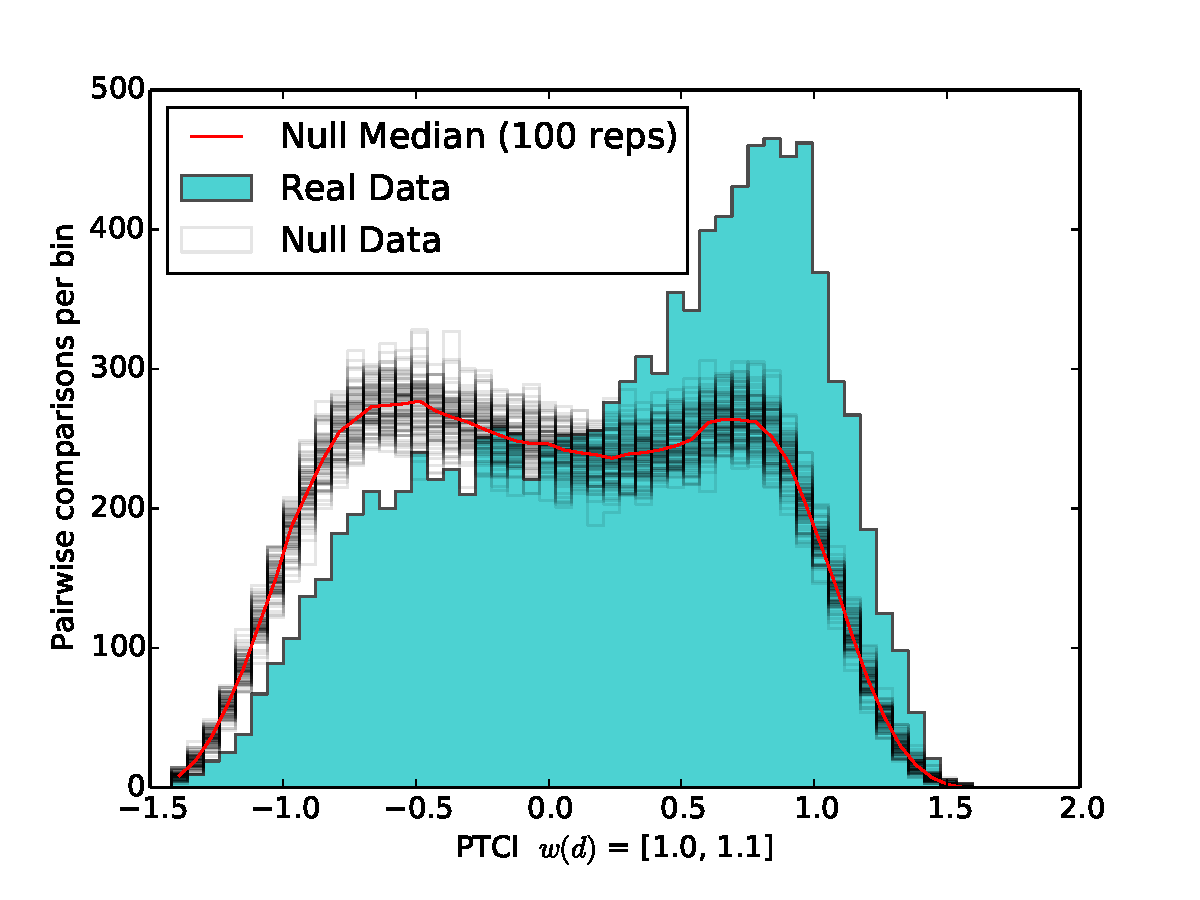
\includegraphics[width=.5\linewidth]{figures/figs/ecr_team_ptci_20130918_orthodb7/pairwise_ptci_hist.pdf}}
% 
\subcaptionbox{\label{fig:ecr-pair-ptci-hists-rcum-hist}}
{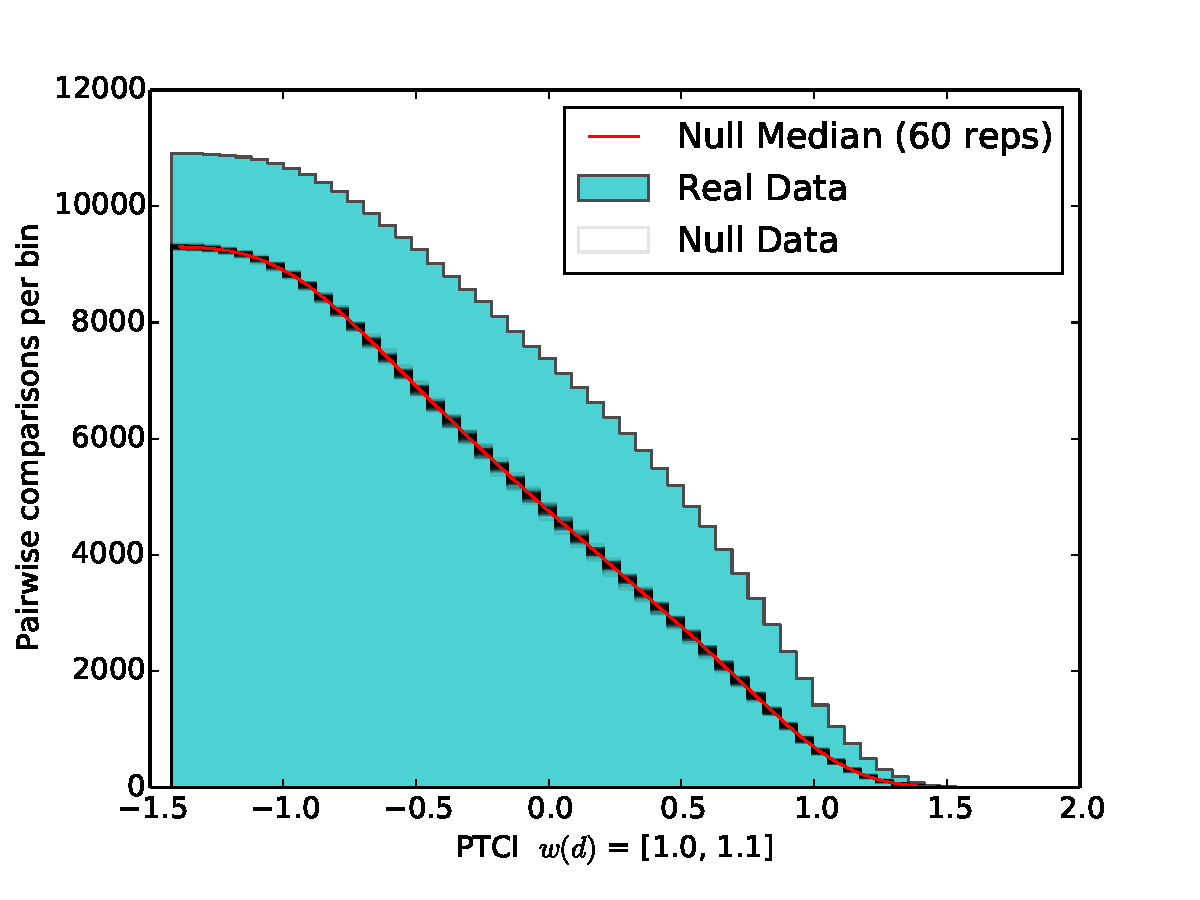
\includegraphics[width=.5\linewidth]{figures/figs/ecr_team_ptci_20130918_orthodb7/pairwise_ptci_cum_hist.pdf}}
% 
\subcaptionbox{\label{fig:ecr-pair-ptci-hists-fdr}}
{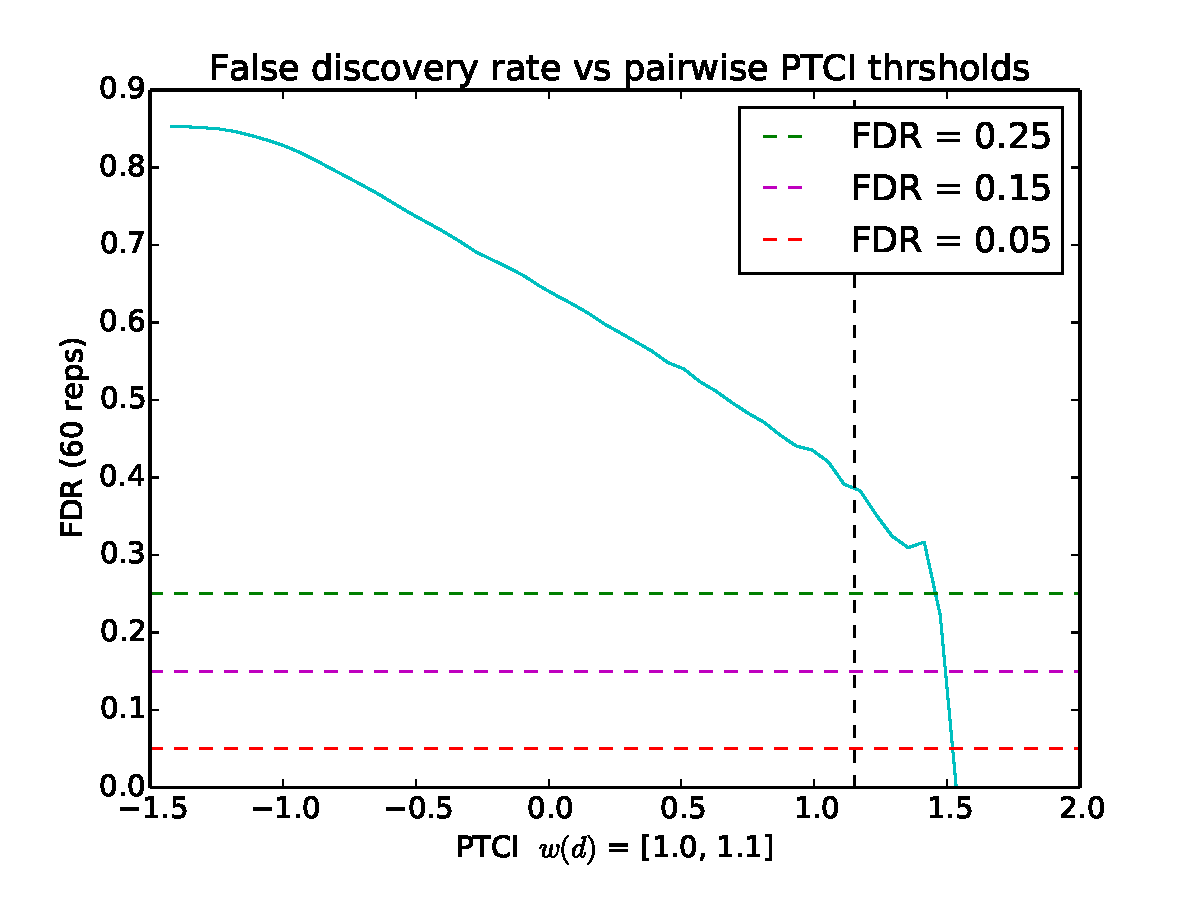
\includegraphics[width=.5\linewidth]{figures/figs/ecr_team_ptci_20130918_orthodb7/pairwise_ptci_fdr.pdf}}
% 
% 
\caption[Pairwise 20E-PTCI results]{\sf \textbf{Pairwise PTCI results for the \gls{20E}-\gls{TFBS} group}:\\
\textbf{(A)} Histogram of mean PTCI results vs null distributions.
\textbf{(B)} Reverse Cumulative histogram of mean PTCI results vs null distributions.
\textbf{(C)} False discover rate vs PTCI threshold.}
\label{fig:ecr-pair-ptci-hists}
\end{figure}
% EcR-pair (Figure \ref{fig:ecr-pair-ptci-hists})

\begin{figure}[hp]
%
\subcaptionbox{\label{fig:ecr-mean-ptci-hists-base}}
{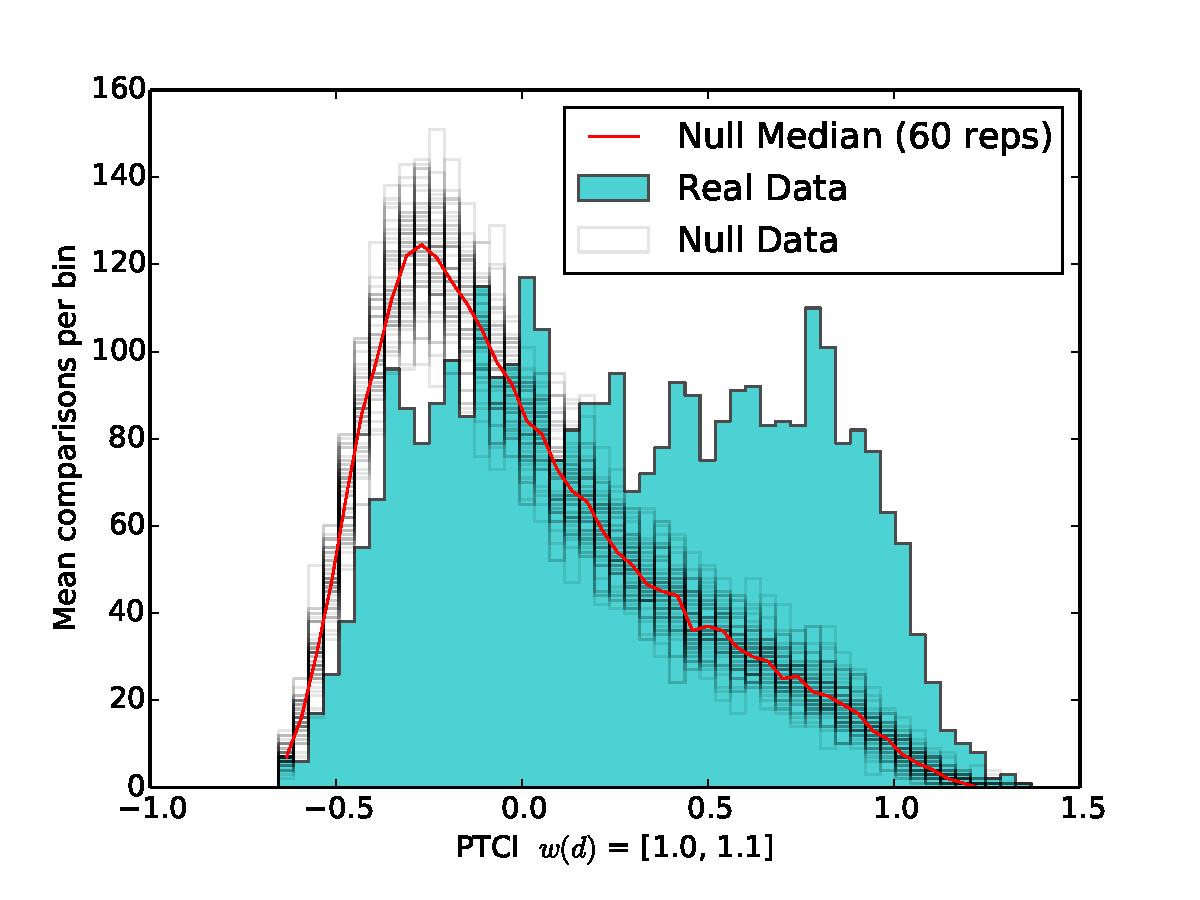
\includegraphics[width=.5\linewidth]{figures/figs/ecr_team_ptci_20130918_orthodb7/mean_ptci_hist.pdf}}
% 
\subcaptionbox{\label{fig:ecr-mean-ptci-hists-rcum-hist}}
{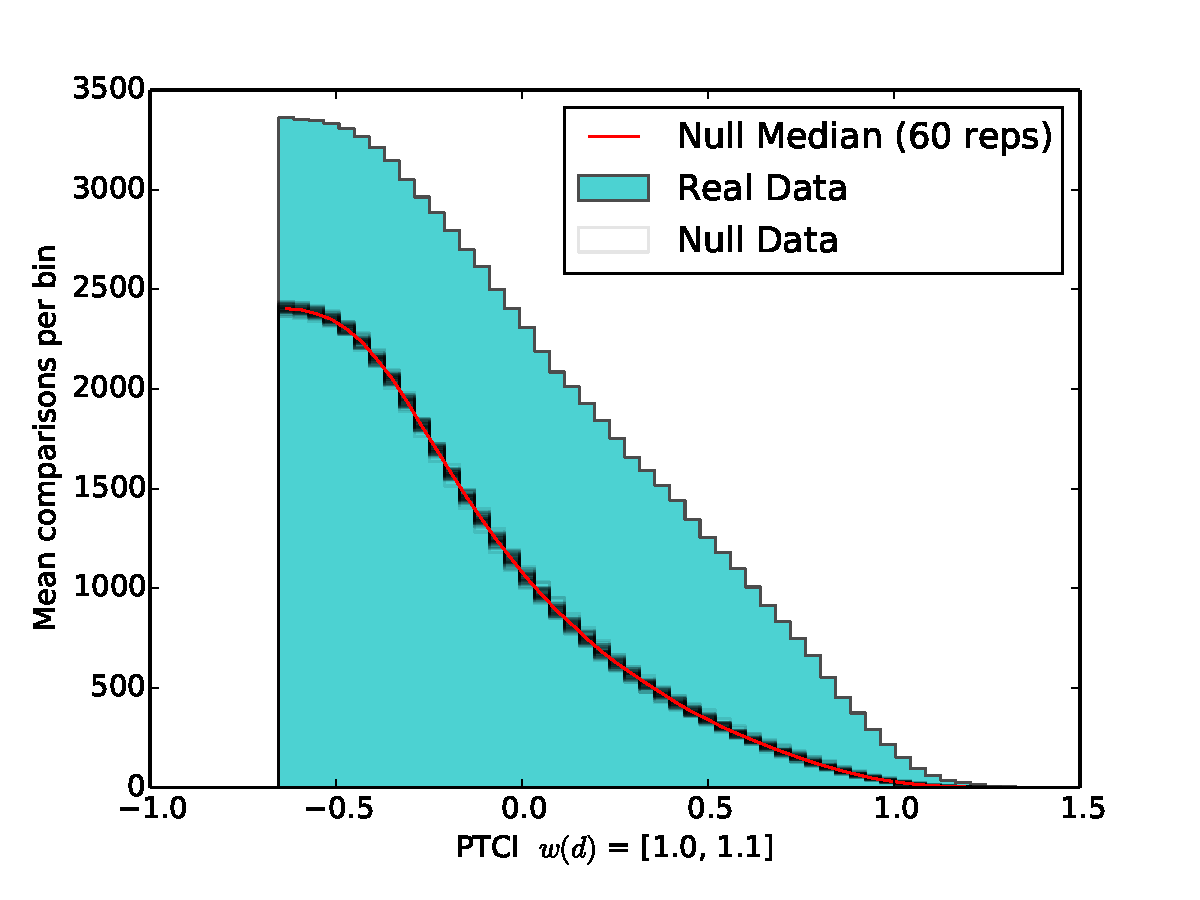
\includegraphics[width=.5\linewidth]{figures/figs/ecr_team_ptci_20130918_orthodb7/mean_ptci_cum_hist.pdf}}
% 
\subcaptionbox{\label{fig:ecr-mean-ptci-hists-fdr}}
{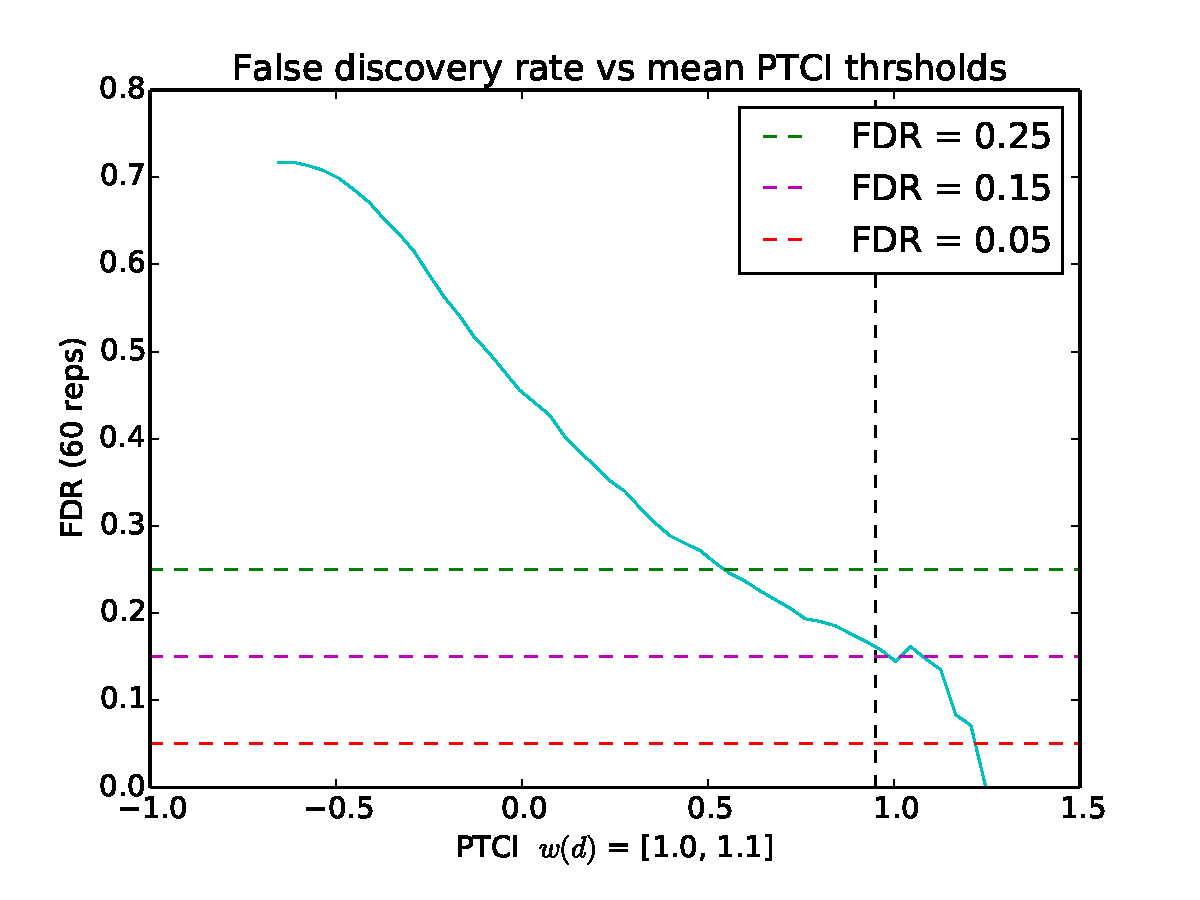
\includegraphics[width=.5\linewidth]{figures/figs/ecr_team_ptci_20130918_orthodb7/mean_ptci_fdr.pdf}}
% 
% 
\caption[Mean 20E-PTCI results]{\sf \textbf{Mean PTCI results for the \gls{20E}-\gls{TFBS} group}:\\
\textbf{(A)} Histogram of mean PTCI results vs null distributions.
\textbf{(B)} Reverse Cumulative histogram of mean PTCI results vs null distributions.
\textbf{(C)} False discovery rate vs PTCI threshold.}
\label{fig:ecr-mean-ptci-hists}
\end{figure}
% EcR-mean (Figure \ref{fig:ecr-mean-ptci-hists})

\begin{figure}[hp]
%
\subcaptionbox{\label{fig:insect-pair-ptci-hists-base}}
{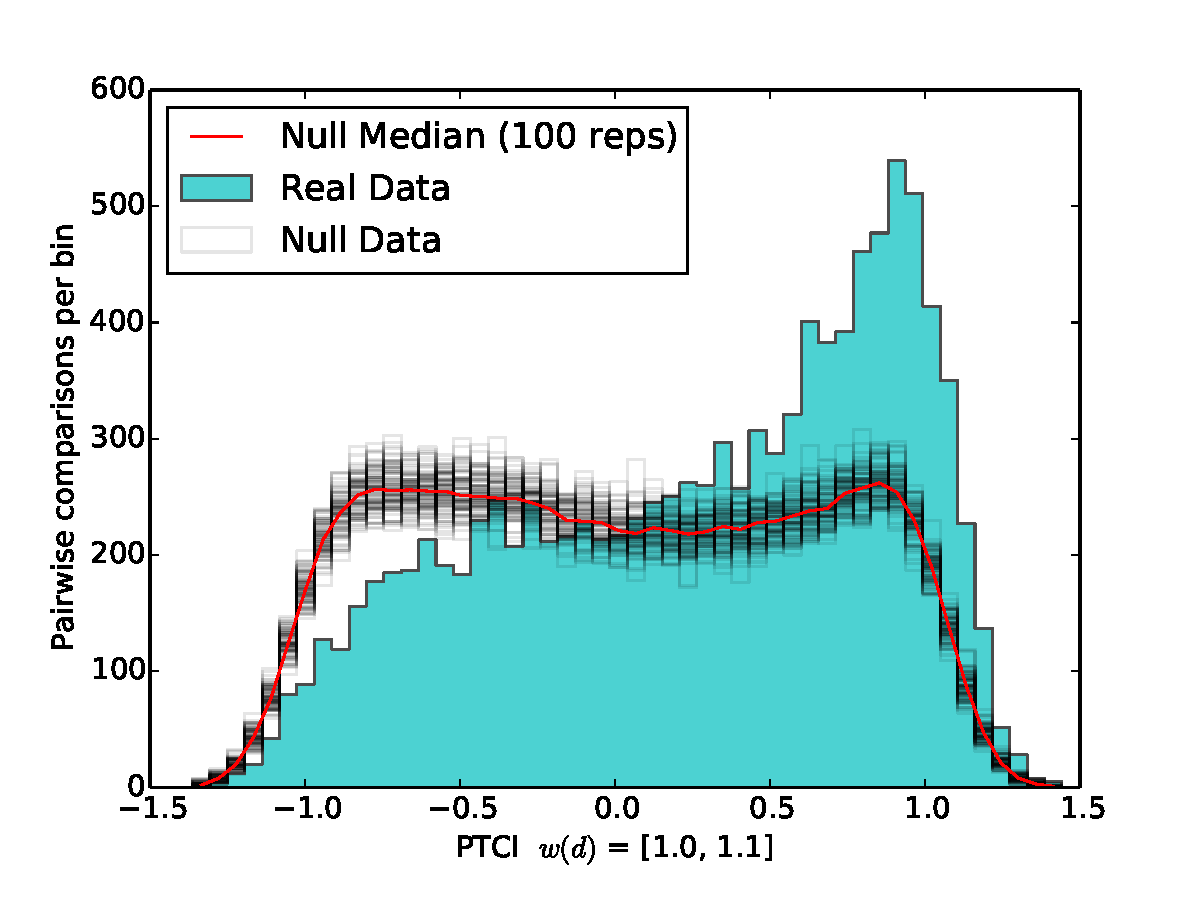
\includegraphics[width=.5\linewidth]{figures/figs/jaspar_insect_ptci_20130918_orthodb7/pairwise_ptci_hist.pdf}}
% 
\subcaptionbox{\label{fig:insect-pair-ptci-hists-rcum-hist}}
{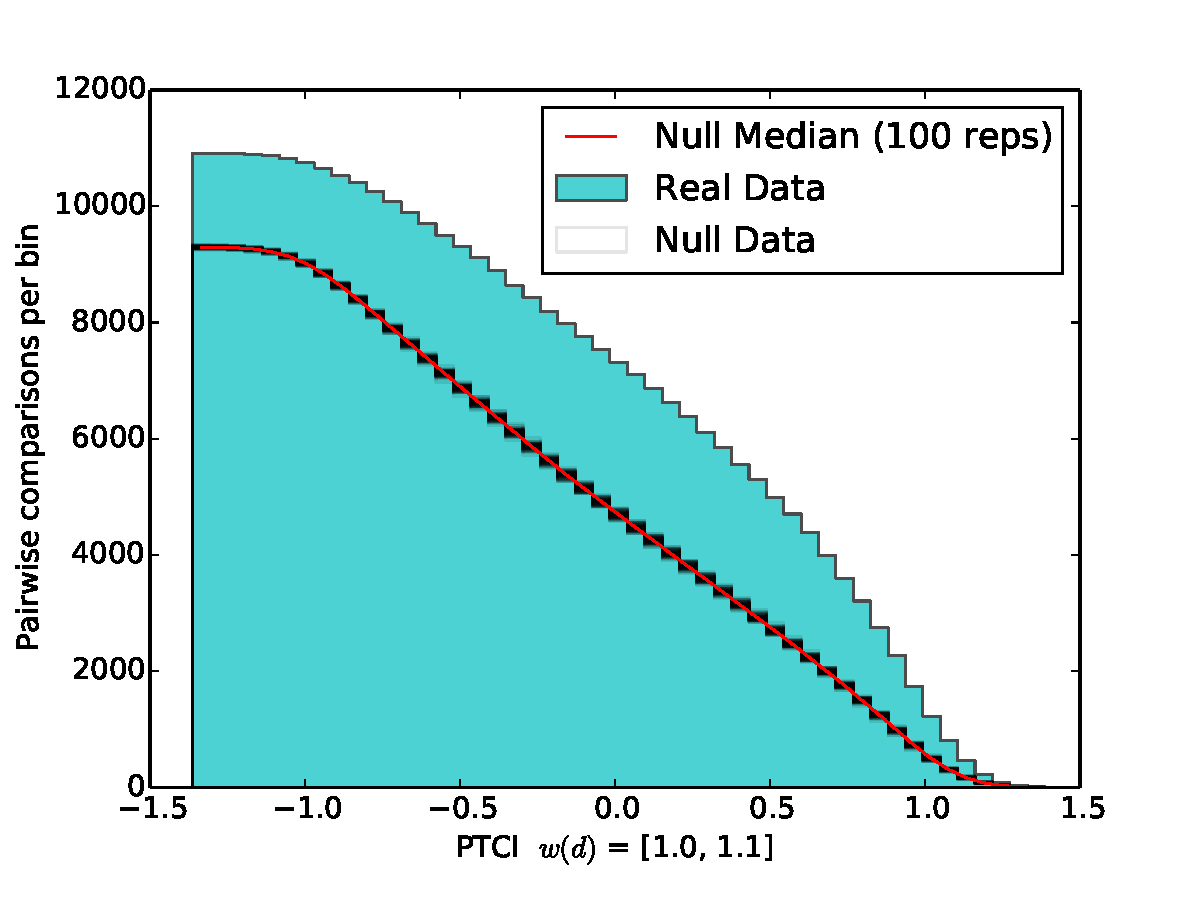
\includegraphics[width=.5\linewidth]{figures/figs/jaspar_insect_ptci_20130918_orthodb7/pairwise_ptci_cum_hist.pdf}}
% 
\subcaptionbox{\label{fig:insect-pair-ptci-hists-fdr}}
{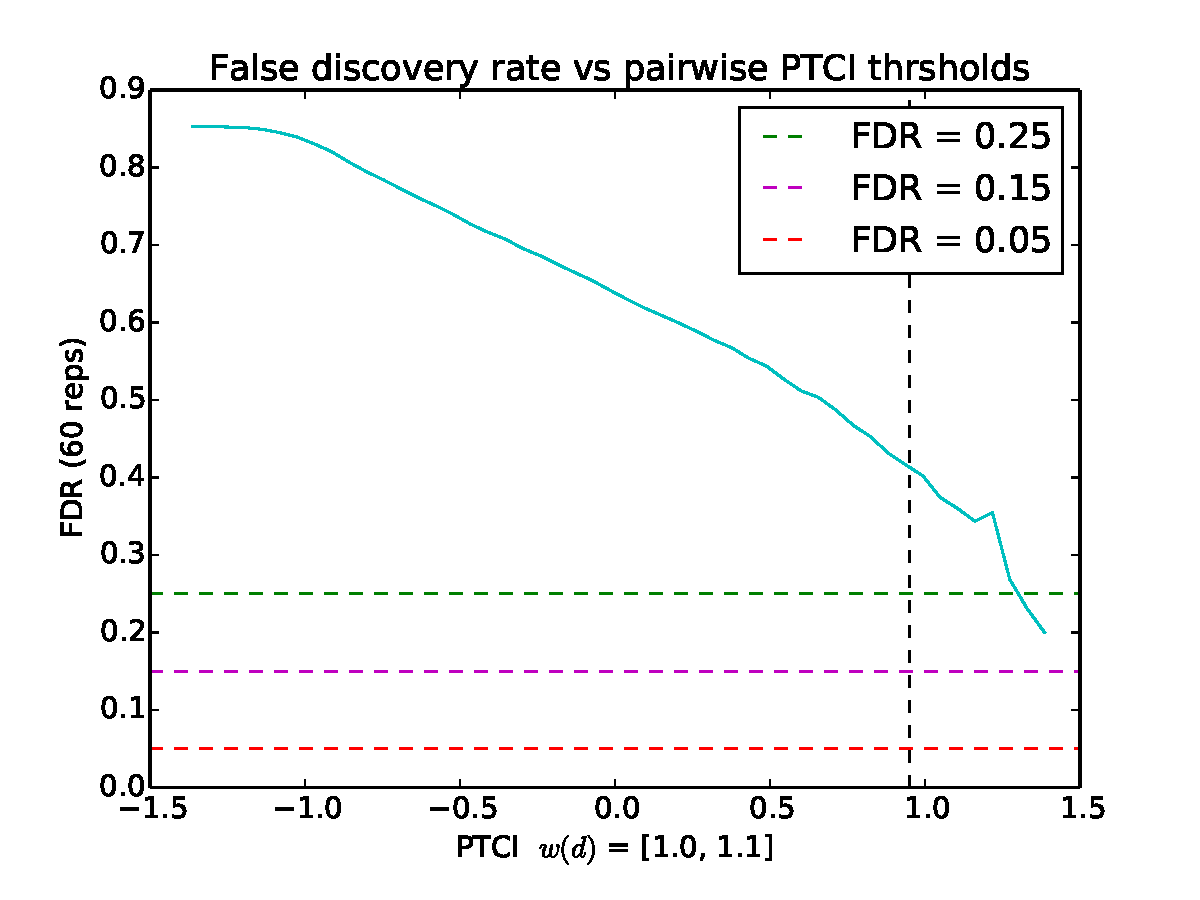
\includegraphics[width=.5\linewidth]{figures/figs/jaspar_insect_ptci_20130918_orthodb7/pairwise_ptci_fdr.pdf}}
% 
% 
\caption[Pairwise insect-PTCI results]{\sf \textbf{Pairwise PTCI results for the insect-\gls{TFBS} group}:\\
\textbf{(A)} Histogram of mean PTCI results vs null distributions.
\textbf{(B)} Reverse Cumulative histogram of mean PTCI results vs null distributions.
\textbf{(C)} False discover rate vs PTCI threshold.}
\label{fig:insect-pair-ptci-hists}
\end{figure}
% Insect-pair (Figure \ref{fig:insect-pair-ptci-hists})

\begin{figure}[hp]
% /home/gus/Dropbox/repos/git/uci-thesis-latex/figures/figs/jaspar_insect_ptci_20130918_orthodb7/mean_ptci_cum_hist.pdf
\subcaptionbox{\label{fig:insect-mean-ptci-hists-base}}
{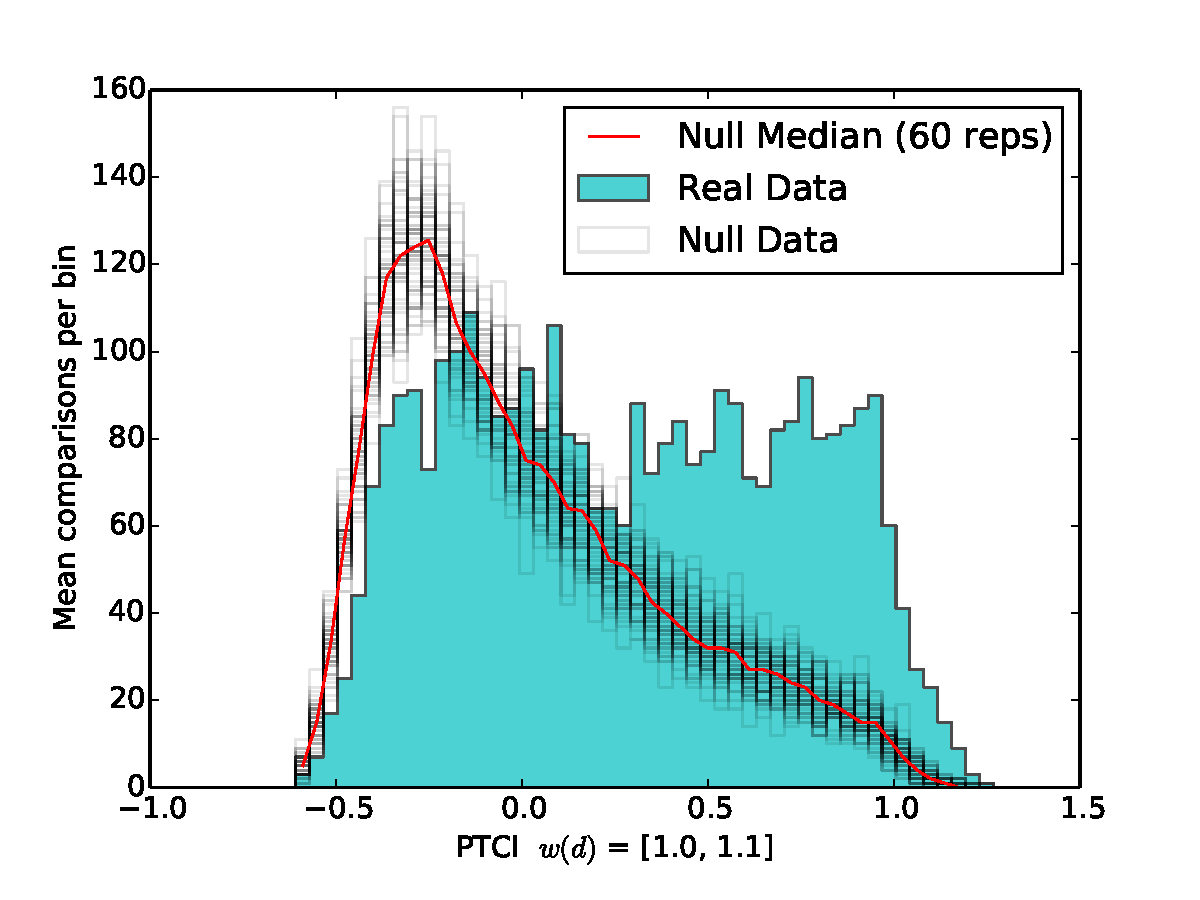
\includegraphics[width=.5\linewidth]{figures/figs/jaspar_insect_ptci_20130918_orthodb7/mean_ptci_hist.pdf}}
% 
\subcaptionbox{\label{fig:insect-mean-ptci-hists-rcum-hist}}
{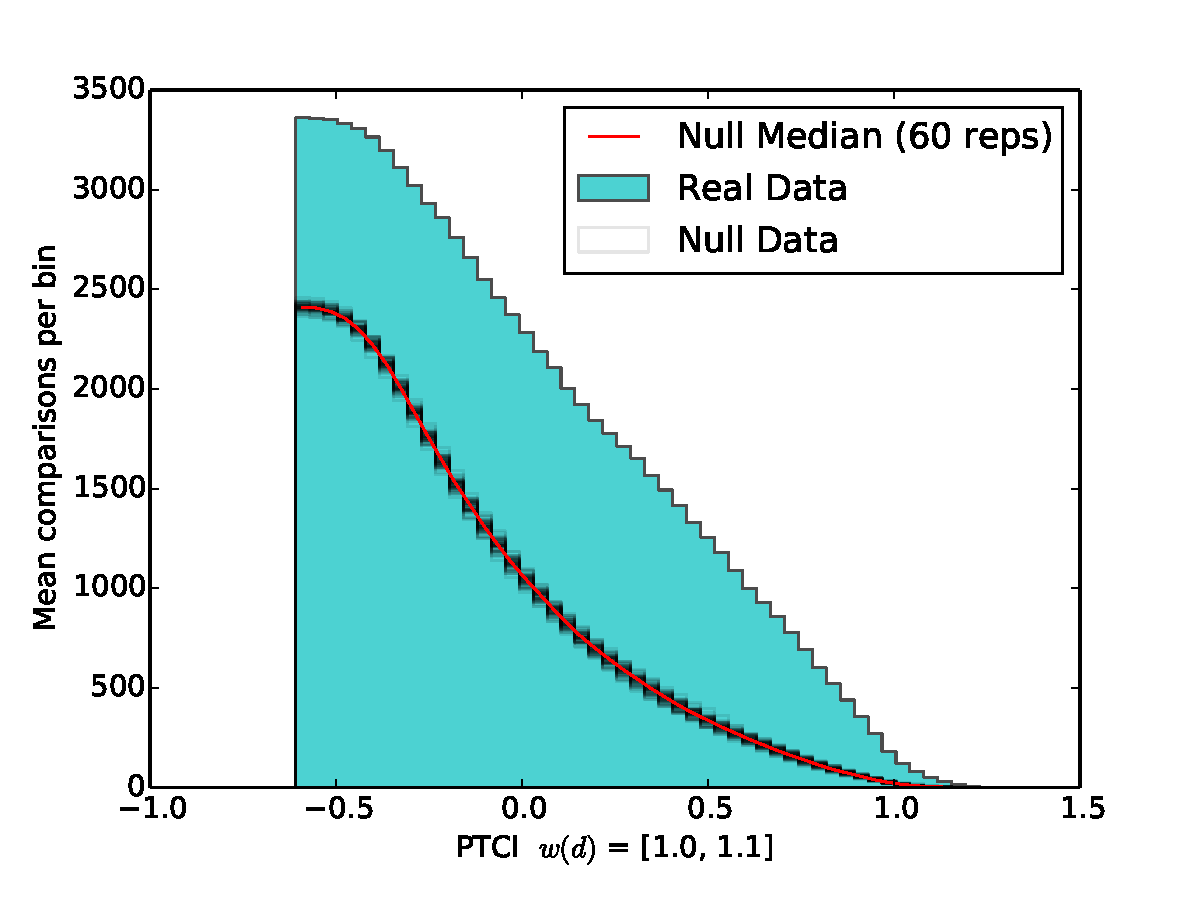
\includegraphics[width=.5\linewidth]{figures/figs/jaspar_insect_ptci_20130918_orthodb7/mean_ptci_cum_hist.pdf}}
% 
\subcaptionbox{\label{fig:insect-mean-ptci-hists-fdr}}
{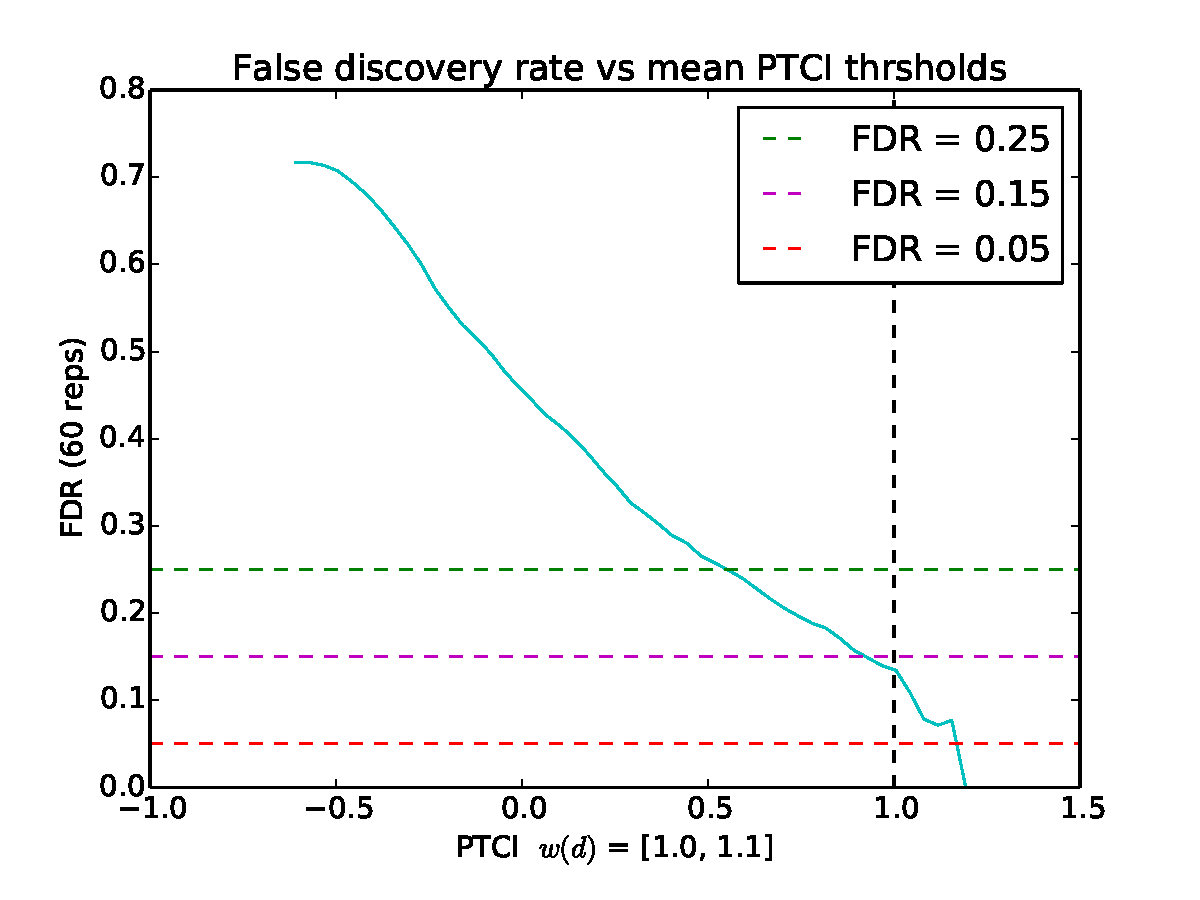
\includegraphics[width=.5\linewidth]{figures/figs/jaspar_insect_ptci_20130918_orthodb7/mean_ptci_fdr.pdf}}
% 
% 
\caption[Mean insect-PTCI results]{\sf \textbf{Mean PTCI results for the insect-\gls{TFBS} group}:\\
\textbf{(A)} Histogram of mean PTCI results vs null distributions.
\textbf{(B)} Reverse Cumulative histogram of mean PTCI results vs null distributions.
\textbf{(C)} False discover rate vs PTCI threshold.}
\label{fig:insect-mean-ptci-hists}
\end{figure}
% Insect-mean (Figure \ref{fig:insect-mean-ptci-hists})

These results pertain to the second stage of the approach described in Chapter \ref{chap:3} (Figure \ref{fig:approach-chart}: \textit{yellow box}).

\paragraph*{Complementary sets of TFBS models:}
\gls{PTCI} data was calculated using two complementary sets of \gls{TFBS} models.
%
One set focuses the \gls{PTCI} on genes that have been associated with \gls{20E} and its nuclear receptor (\PTCIe) (Figures \ref{fig:ecr-pair-ptci-hists} and \ref{fig:ecr-mean-ptci-hists}), and a second provides a general focus on \gls{TFBS} models provided by JASPAR that are defined in insects at large (\PTCIi) (Figures \ref{fig:insect-pair-ptci-hists} and \ref{fig:insect-mean-ptci-hists}).
%
\FDR\ estimation was used to determine a suitable \PTCI\ value to use as a threshold for further investigating particular 3-way 1:1 ortholog sets.
%
It was determined that in both \gls{TFBS} model data-sets a mean \PTCI\ threshold of 0.95 yielded an \FDR\ of approximately 15\% and maximized the number of genes for further classification (Figures \ref{fig:ecr-mean-ptci-hists-fdr} and \ref{fig:insect-mean-ptci-hists-fdr}).
%
This threshold produced 666 and 708 genes in the \PTCIi\ and \PTCIe\ sets, respectively.
%
The union of these gene-sets was 930 genes or 310 genes from each species.
%
The intersection was 444 or an overlap of 66\% of the \PTCIi\ genes and 62.7\% of the \PTCIe\ genes.
%
The unique proportion contributed by each set are 33\% and 37.3\%, respectively.

\paragraph*{Mean vs pairwise PTCI:}
Comparing the \FDR\ values of the pairwise- and mean-\PTCI\ scores at the 0.95 threshold reveals the impact of considering information from all 3-way 1:1 orthologs simultaneously rather than species-pair by species-pair (Figures \ref{fig:ecr-pair-ptci-hists-fdr} vs \ref{fig:ecr-mean-ptci-hists-fdr} and Figures \ref{fig:insect-pair-ptci-hists-fdr} vs \ref{fig:insect-mean-ptci-hists-fdr}).
%
The quality, as judged by \FDR, is strikingly improved by including the relationships of all three species weighted by their pairwise evolutionary distance: an improvement of approximately 30 percentage points in both cases.

\section{Characterization of Results}
These results pertain to the third stage of the approach described in Chapter \ref{chap:3} (Figure \ref{fig:approach-chart}: \textit{blue box}).

\subsection{Functional annotations (before k-means clustering)}

Functional annotations were obtained for the 930 genes using \gls{Argot2} (Section \ref{chap:3-sec:characterization-of-results}).
%
%% How many of the 930 were assigned at least one annotation >= 200? --> 760 (Aa:253 ,Ag:254 , Cq:253 )
%% How many genes got better than 2000? --> 452 (Aa: 154, Ag:153 , Cq:145 )
Of these, 760 were assigned, by \gls{Argot2}, at least one annotation with a \gls{TS} greater than or equal to 200\footnote{This is the threshold that is suggested by the developers based on their in-house benchmarking \url{http://www.medcomp.medicina.unipd.it/Argot2/help/argot\_scores.php\#ts}} (\Aa: 253, \Ag: 254, \Cq: 253).
%
452 were assigned annotations with \glspl{TS} greater than or equal to 2000 (\Aa: 154, \Ag: 153, \Cq: 145).
%
This indicates that on the whole, most of the 930 genes produced by the \gls{gFunc} process were assigned annotations of a quality at least as stringent as used by the developers of \gls{Argot2}.

%%%%%%%%%%%%%%%%%%%%%


\begin{landscape}

    \begin{figure}[h]
    \centering
    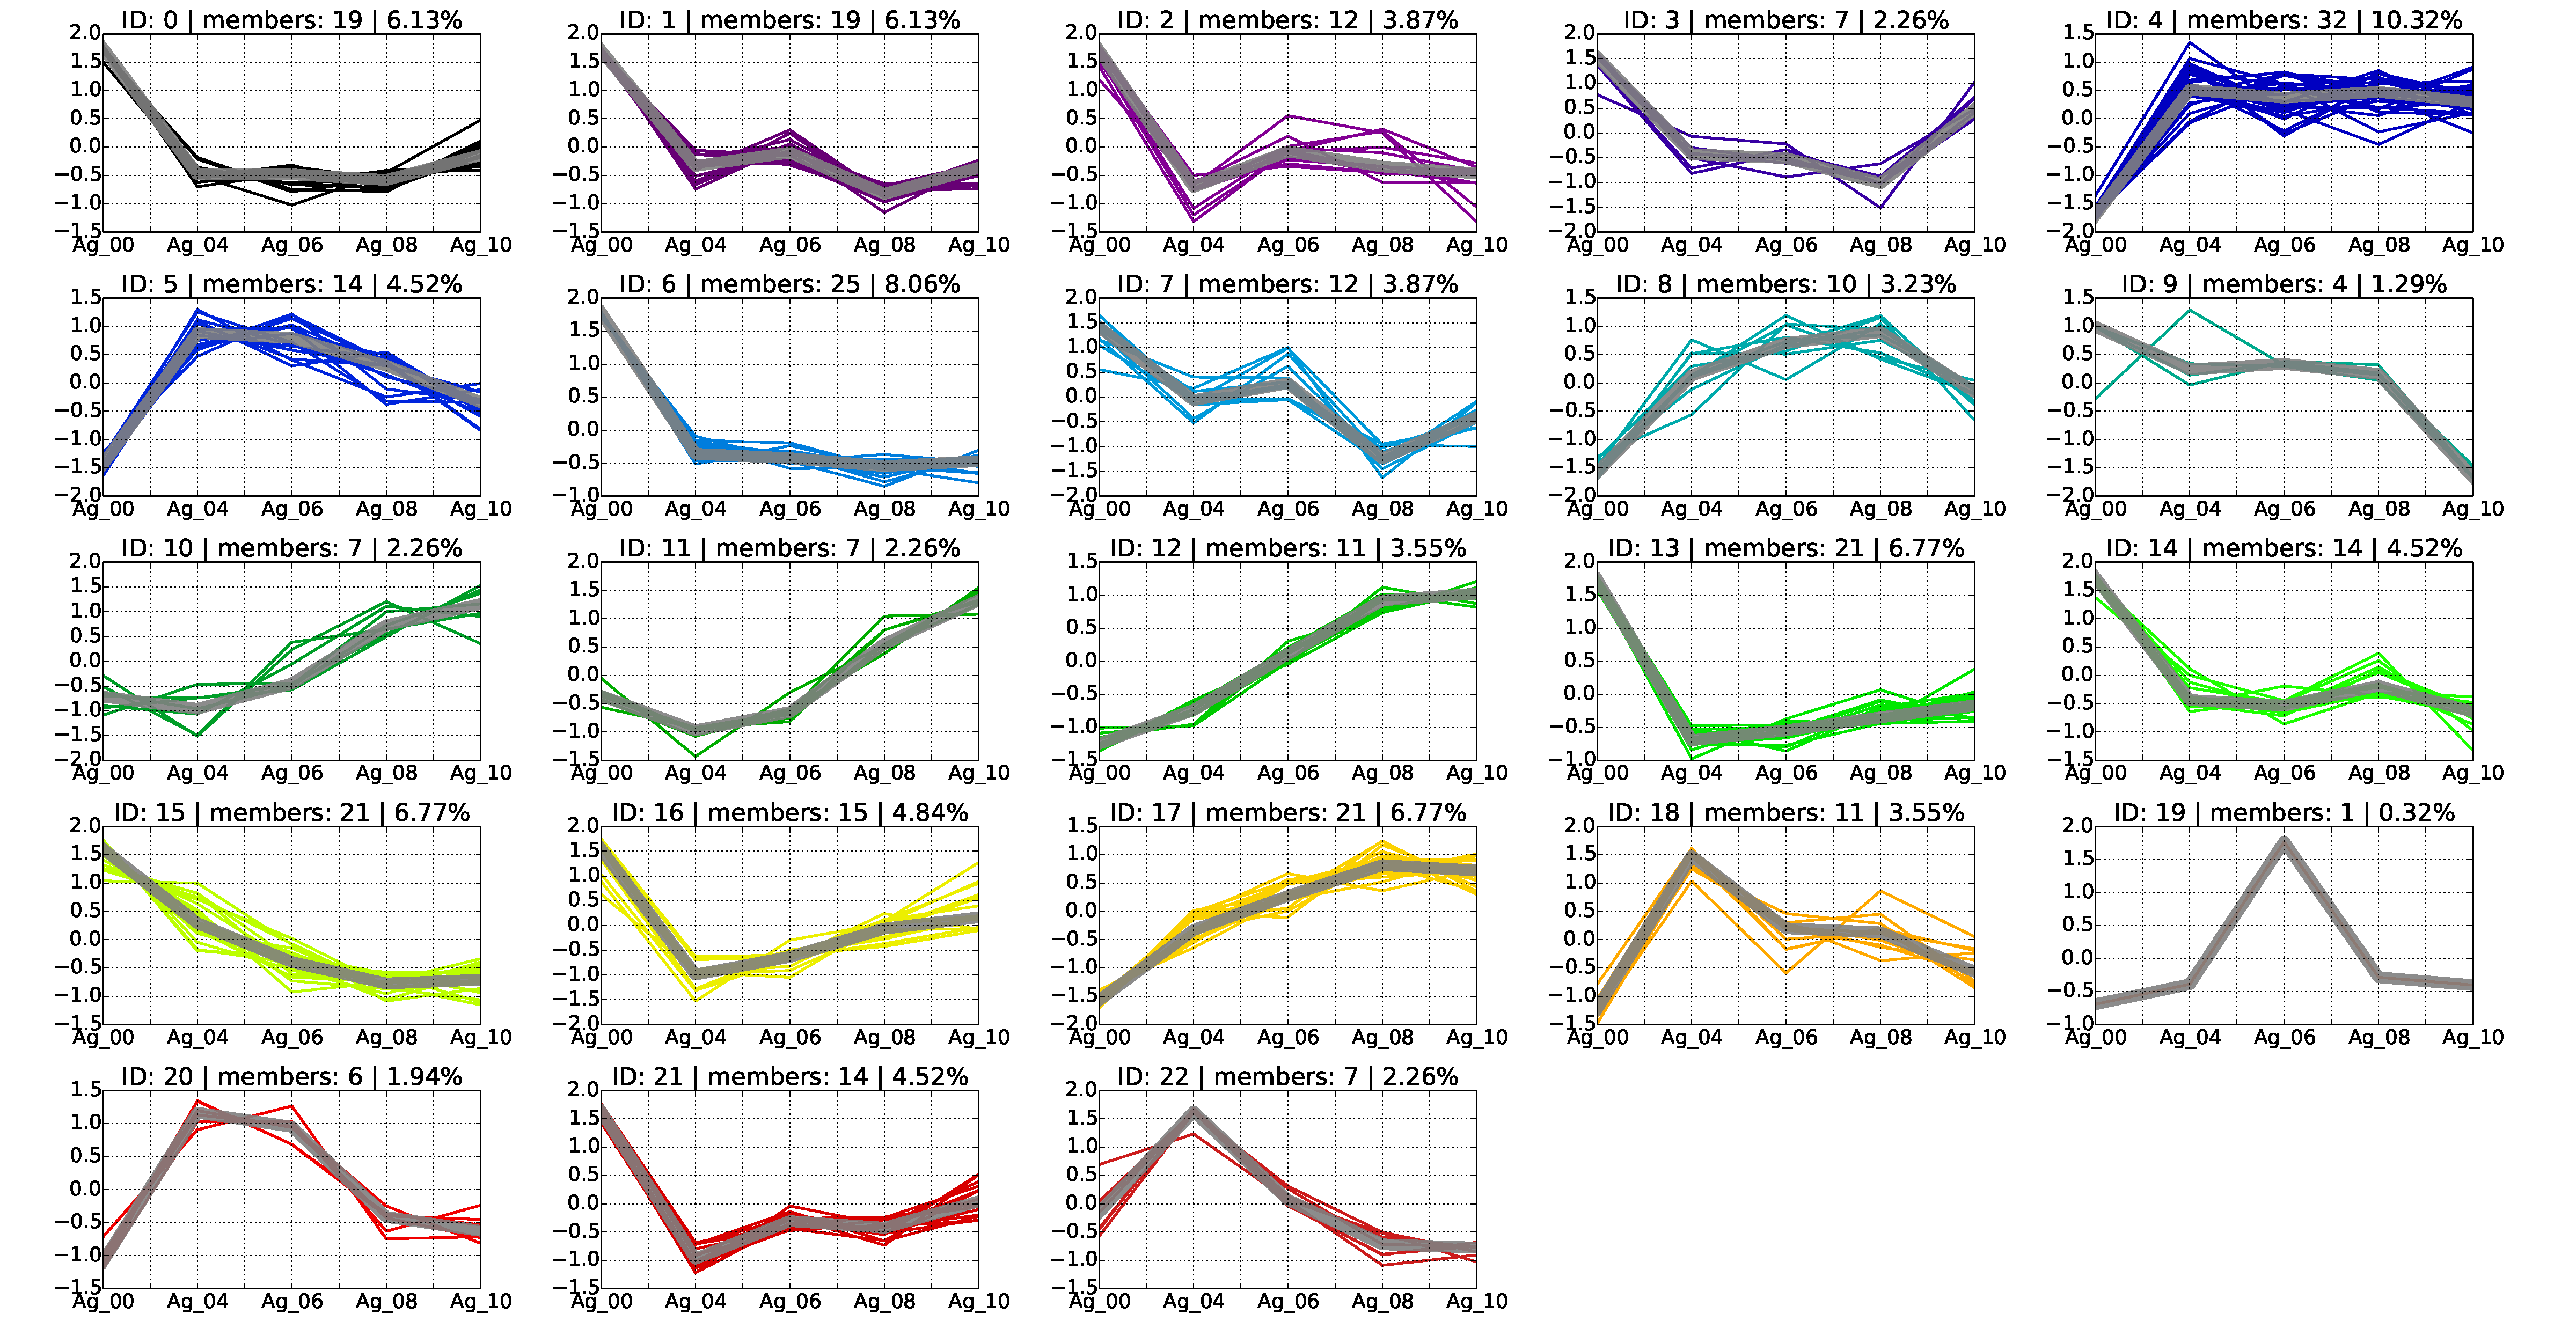
\includegraphics[width=\linewidth]{figures/figs/ecr_and_insects_ptci_20130918_orthodb7/23clusters_ptci_0_95_orthodb7.pdf}
    \caption[\Ag\ clustered abundance profiles]{\sf \textbf{\Ag\ clustered abundance profiles.} \\ 
    Clusters were generated using k-means clustering as implemented in Biopython version 1.62 \cite{Cock2009}.  Abundance profile data was log transformed after one FPKM was added to all data to remove zeros ($log_{10}(\mathrm{FPKM}+1)$).  K-means was then applied using the arithmetic mean as the center for cluster definition.  The data displayed here is the gene-wise standardization of the \textbf{raw} FPKM data such that each profile has mean = 0 and standard deviation = 1. Each median abundance profile is marked by a thick gray line. \textbf{Panel Titles} - ID: cluster identifier | members: number of genes in cluster | percentage of genes represented in all clusters. \textbf{Time Points} - \gls{NBF}, 4, 6, 8, 10 h \gls{PBM}.
}
    \label{fig:23-clusters}
    \end{figure}
    
\end{landscape}


\begin{figure}[p]
% 
\subcaptionbox{\label{fig:cluster4-Aa}}
{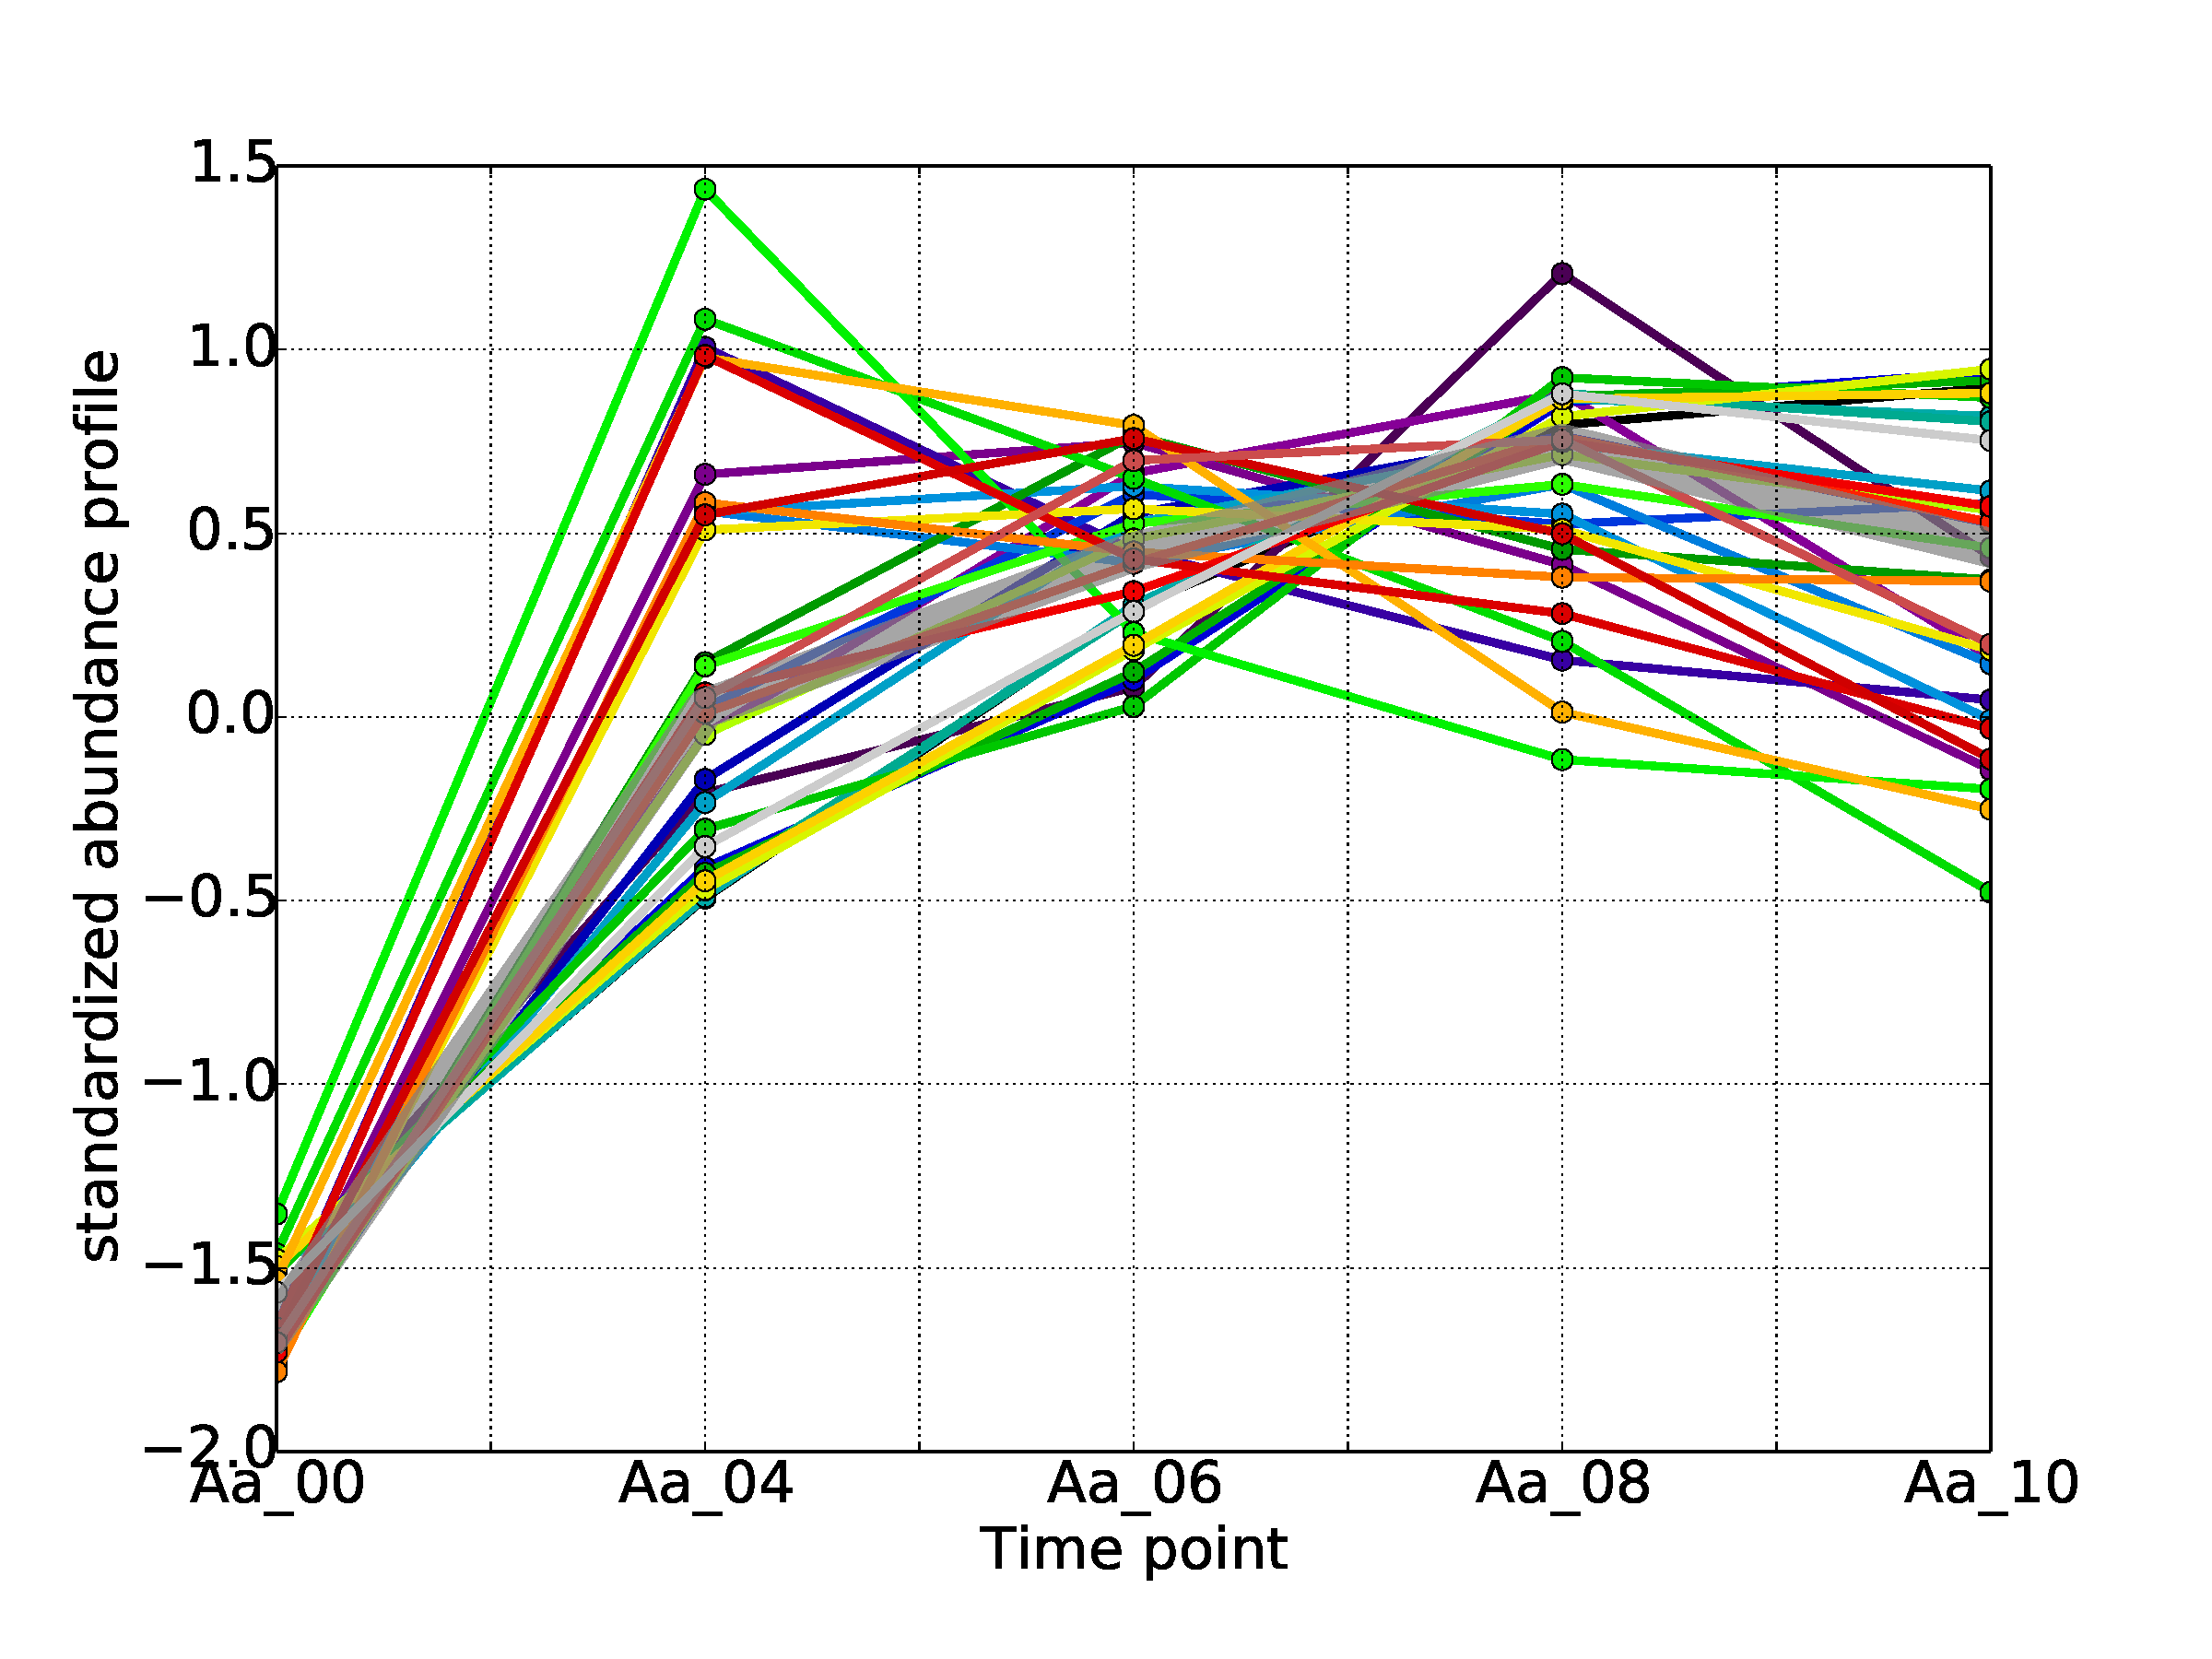
\includegraphics[width=.5\linewidth]{figures/figs/ecr_and_insects_ptci_20130918_orthodb7/upAfter4_gene_profiles_from_cummerbund/Aa_upAfter4_cls4_Ag_target_FPKMs_vb_orthos.pdf}}
%
\subcaptionbox{\label{fig:cluster4-Ag}}
{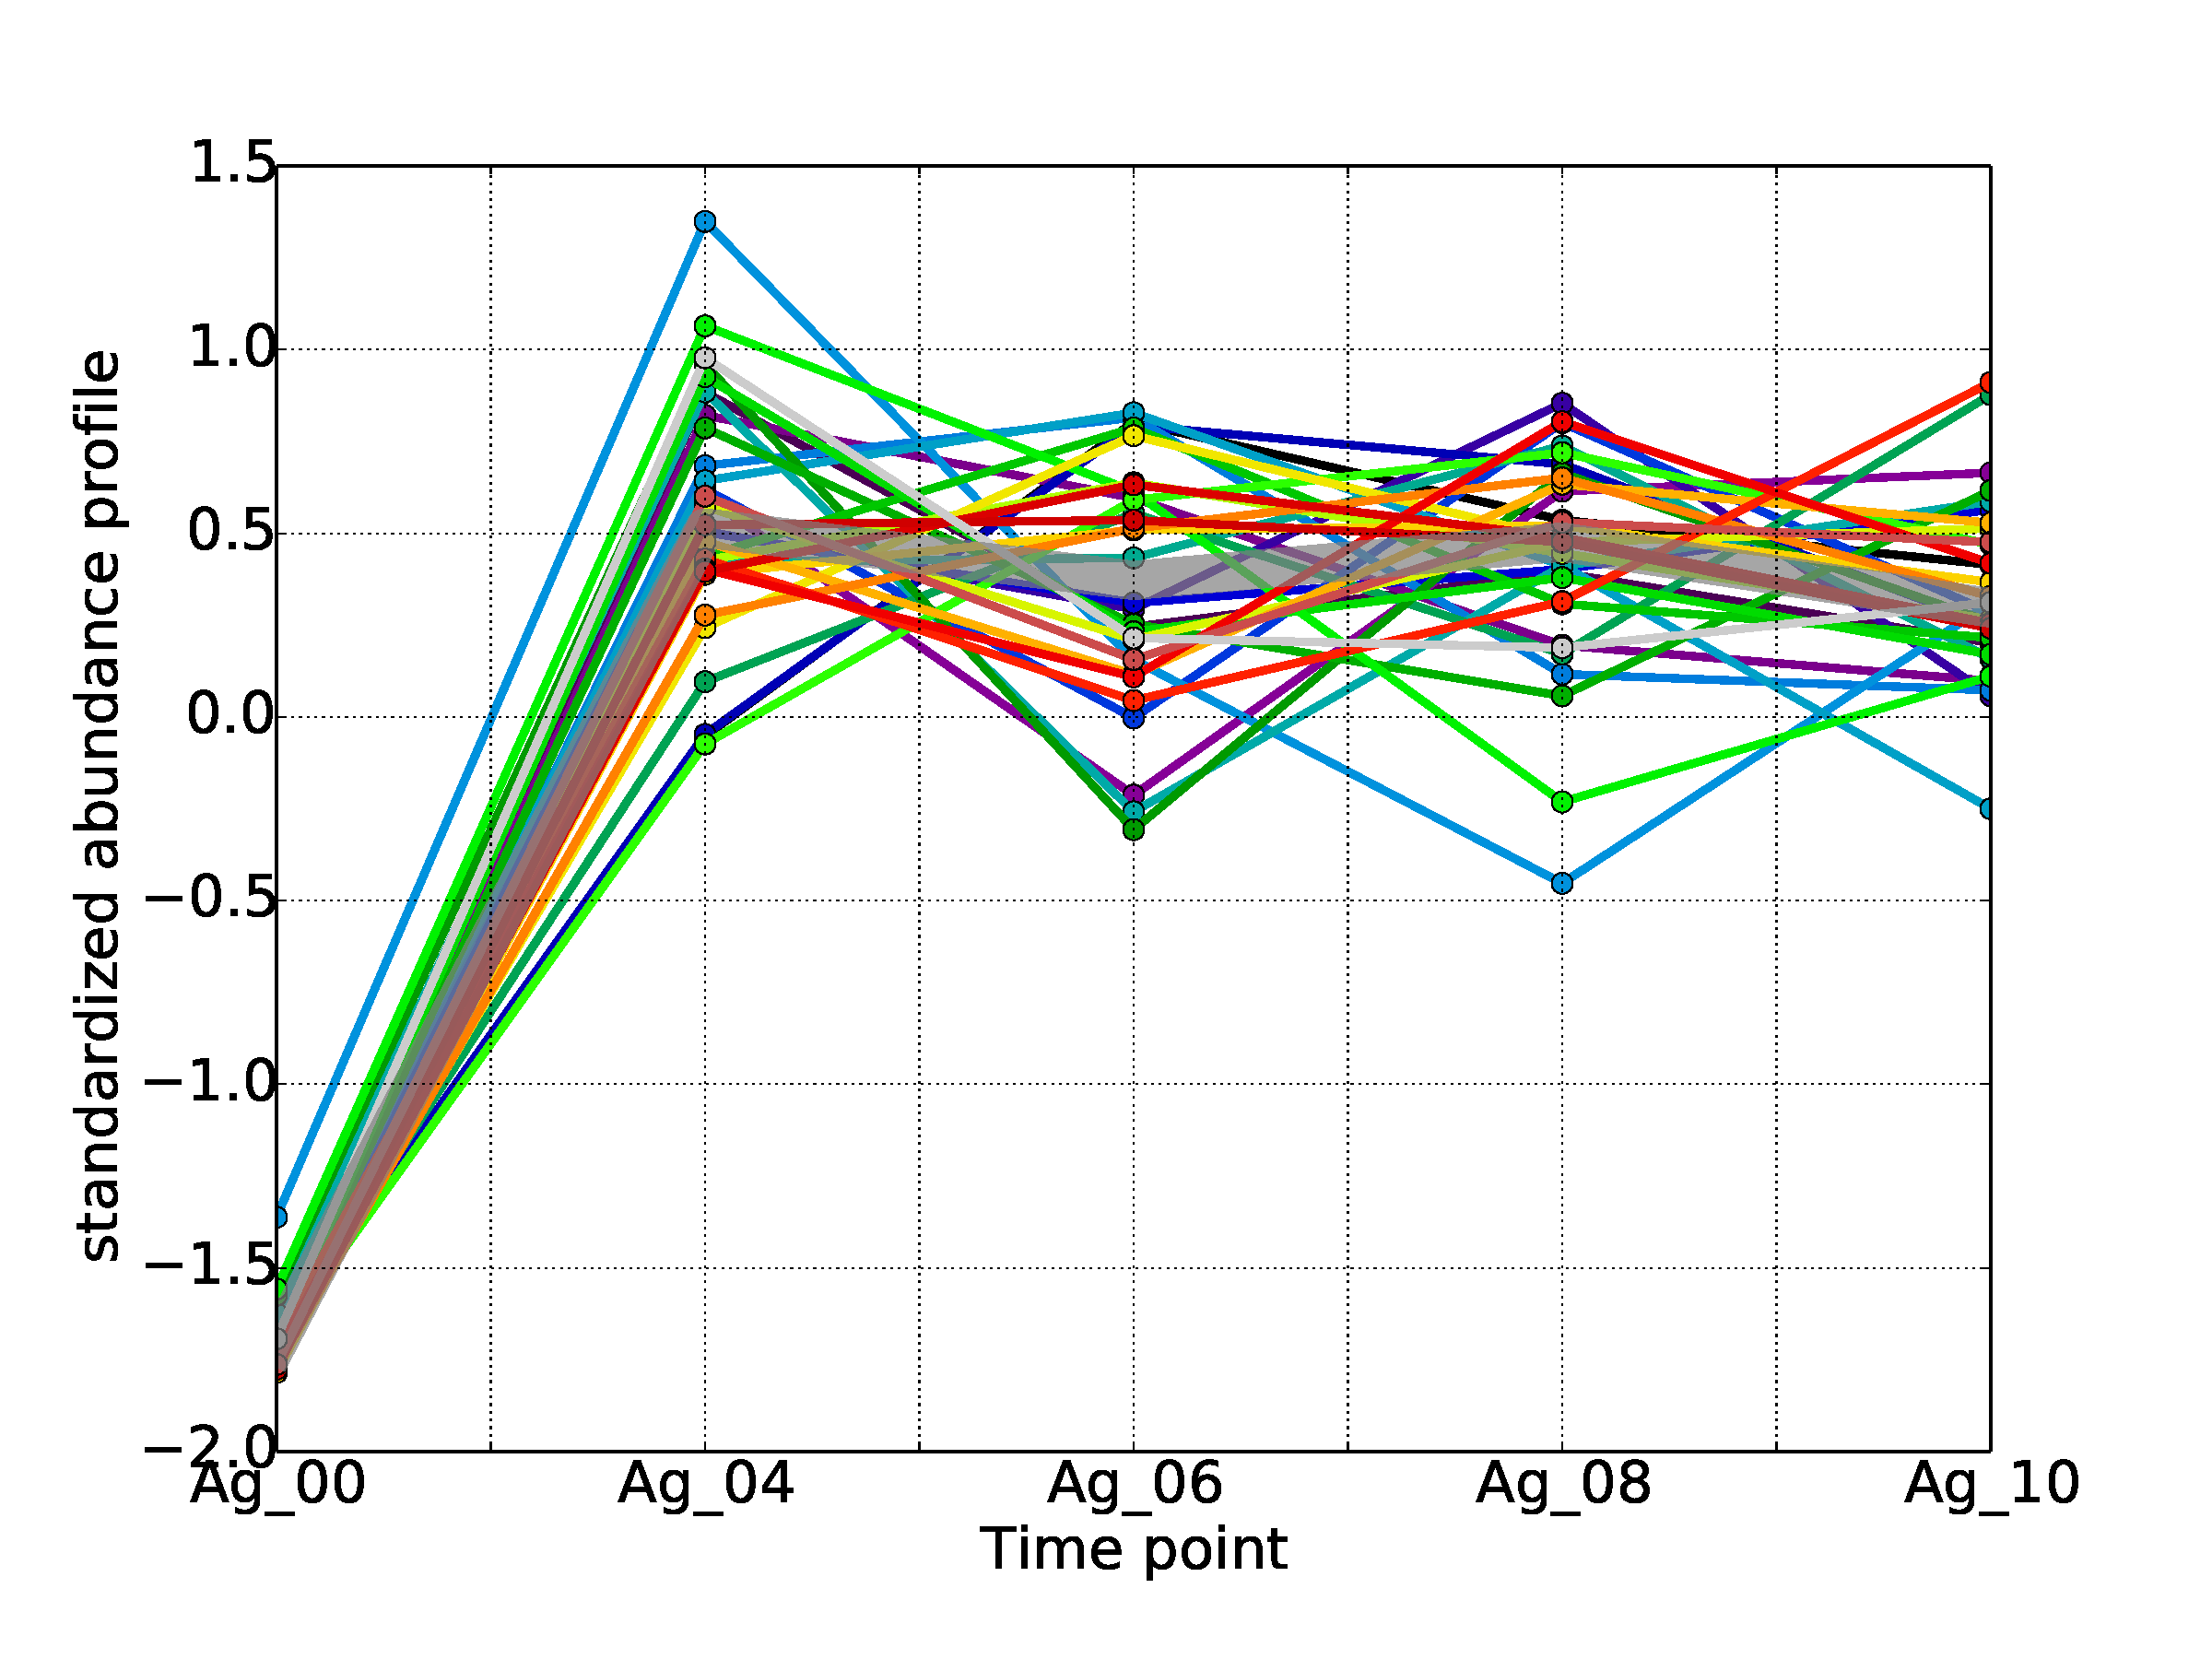
\includegraphics[width=.5\linewidth]{figures/figs/ecr_and_insects_ptci_20130918_orthodb7/upAfter4_gene_profiles_from_cummerbund/Ag_upAfter4_cls4_Ag_target_FPKMs_vb_orthos.pdf}}
%
\subcaptionbox{\label{fig:cluster4-Cq}}
{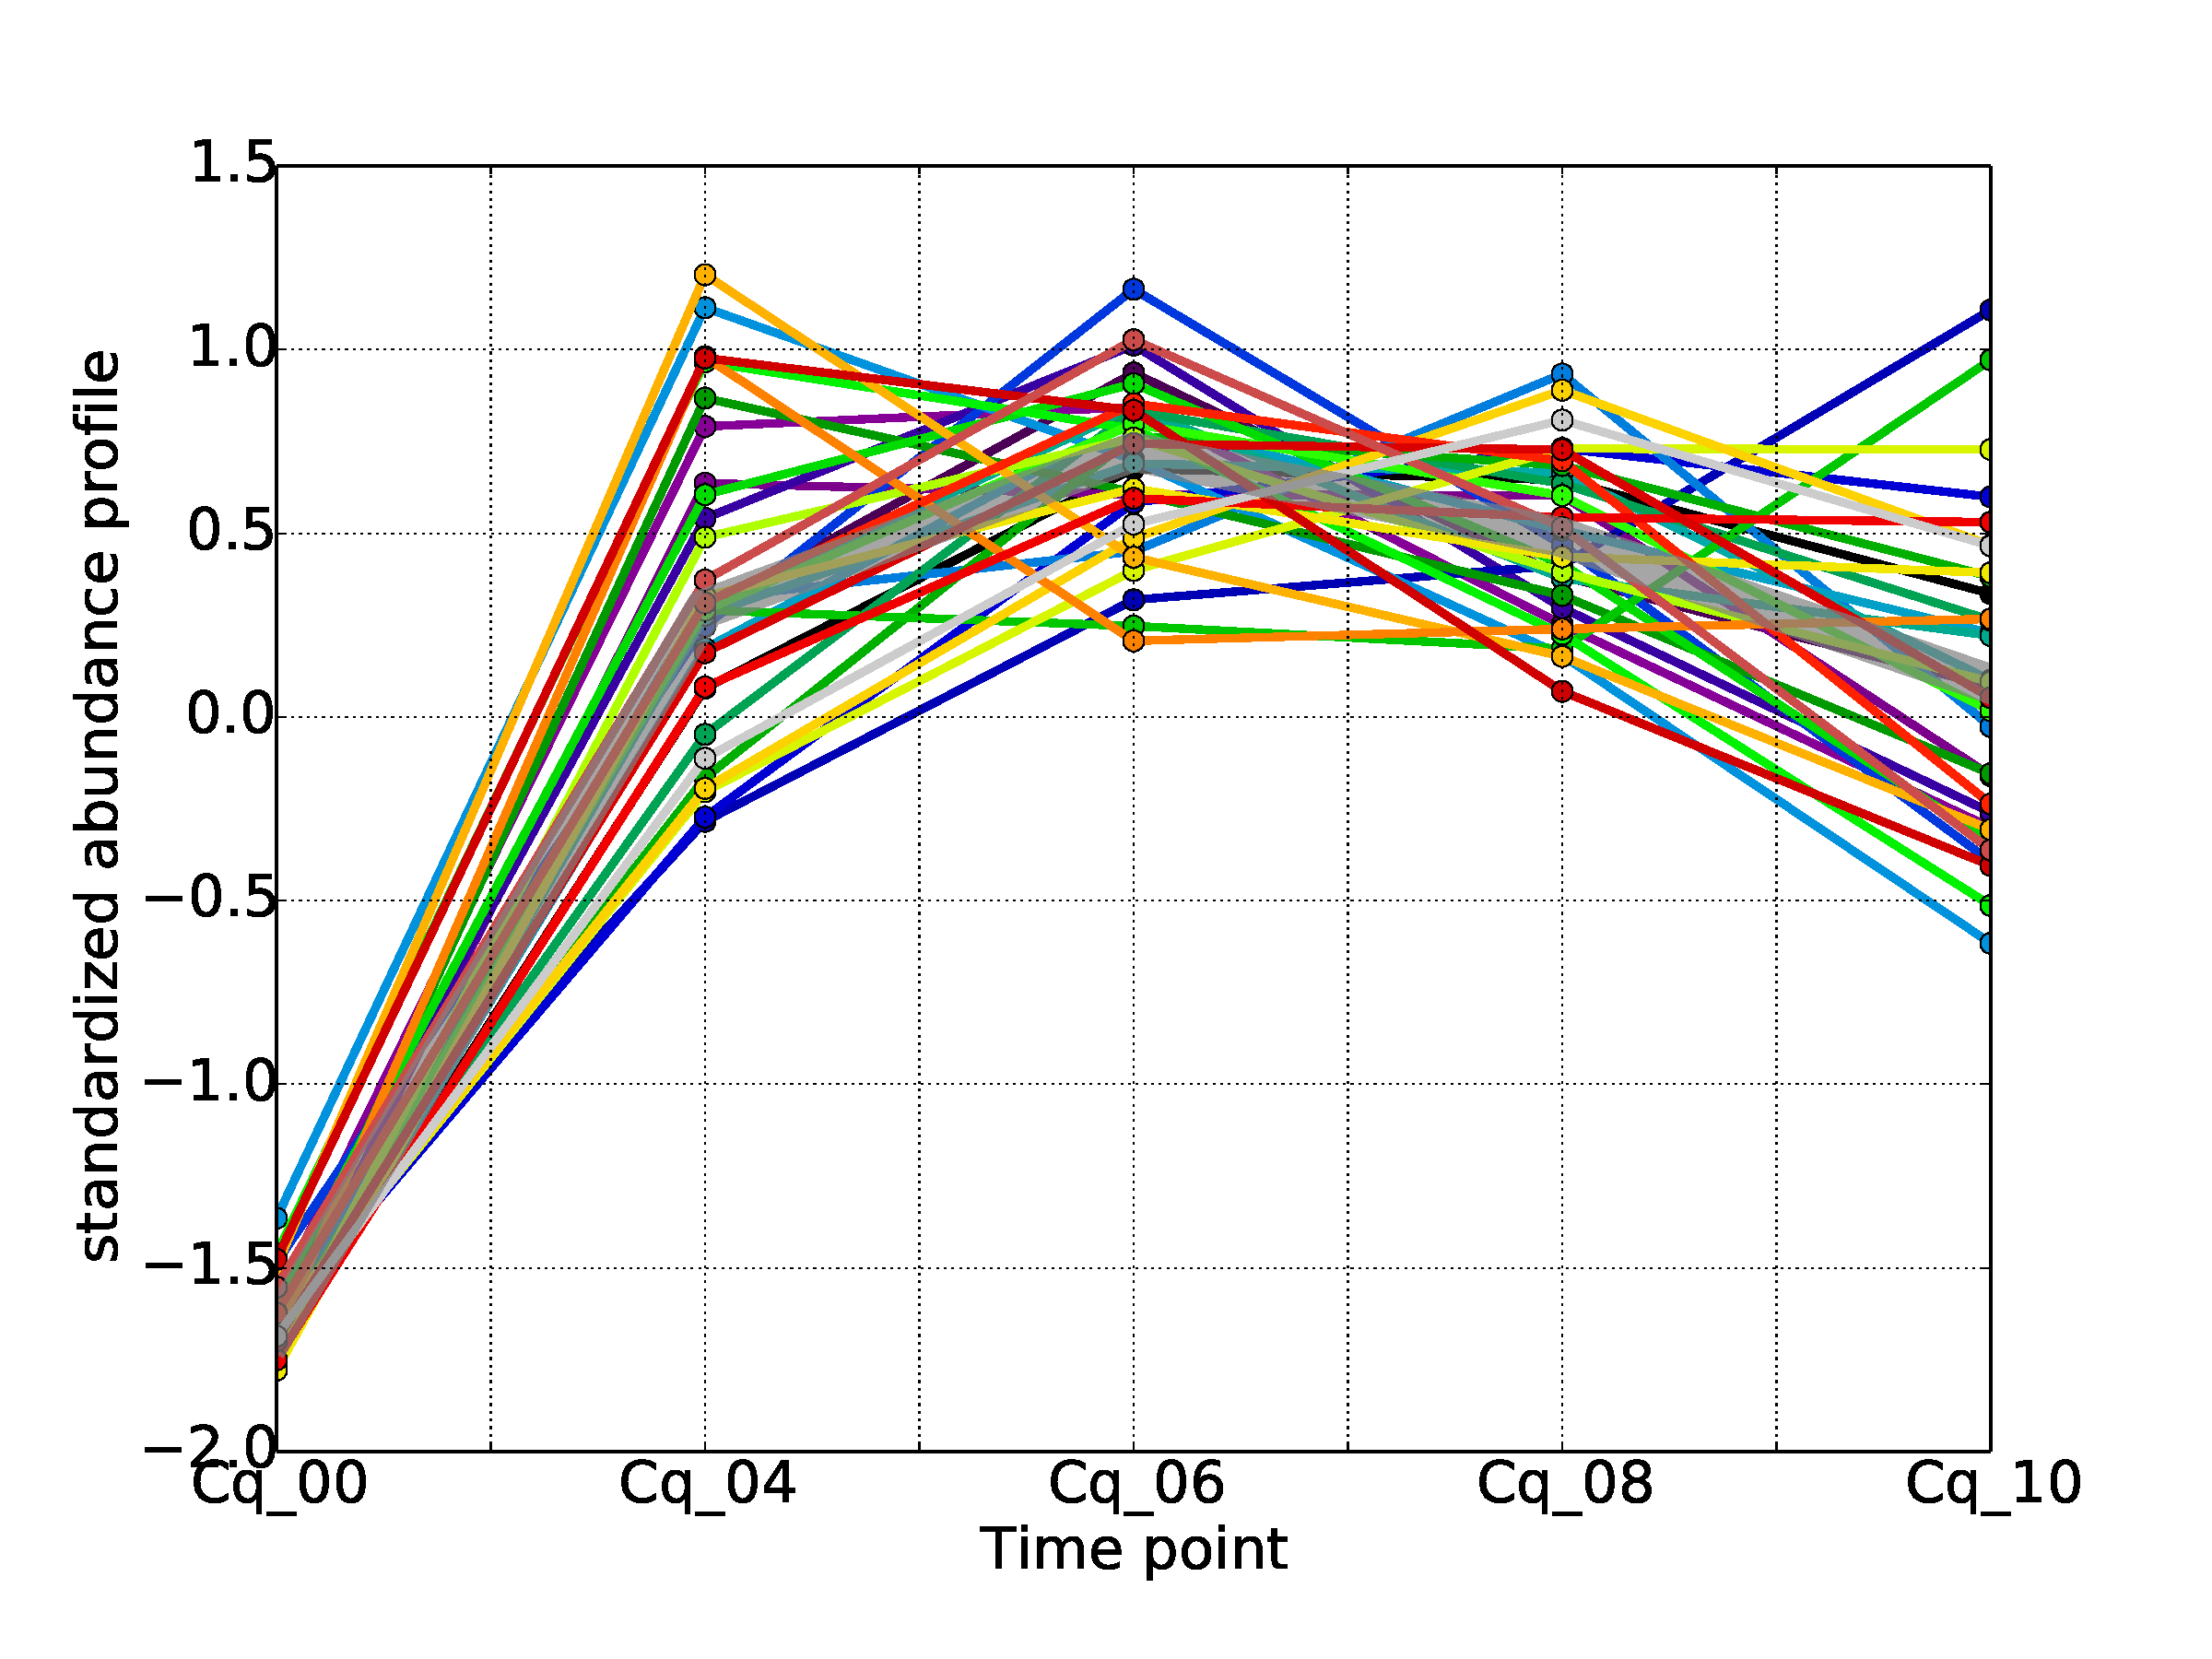
\includegraphics[width=.5\linewidth]{figures/figs/ecr_and_insects_ptci_20130918_orthodb7/upAfter4_gene_profiles_from_cummerbund/Cq_upAfter4_cls4_Ag_target_FPKMs_vb_orthos.pdf}}
% 
\caption[Orthologs of cluster 4]{\sf \textbf{Orthologs of cluster 4 (up after 4h):}\\
The same color scheme is used for each species which means that orthologs are given the same color in all three panels.
The thick, transparent gray line represents the median \gls{mAP} for the panel.
\textbf{(A)} \Aa.
\textbf{(B)} \Ag.
\textbf{(C)} \Cq.
}\label{fig:cluster4}
\end{figure}

\begin{figure}[hp]
% 
\subcaptionbox{\label{fig:cluster6-Aa}}
{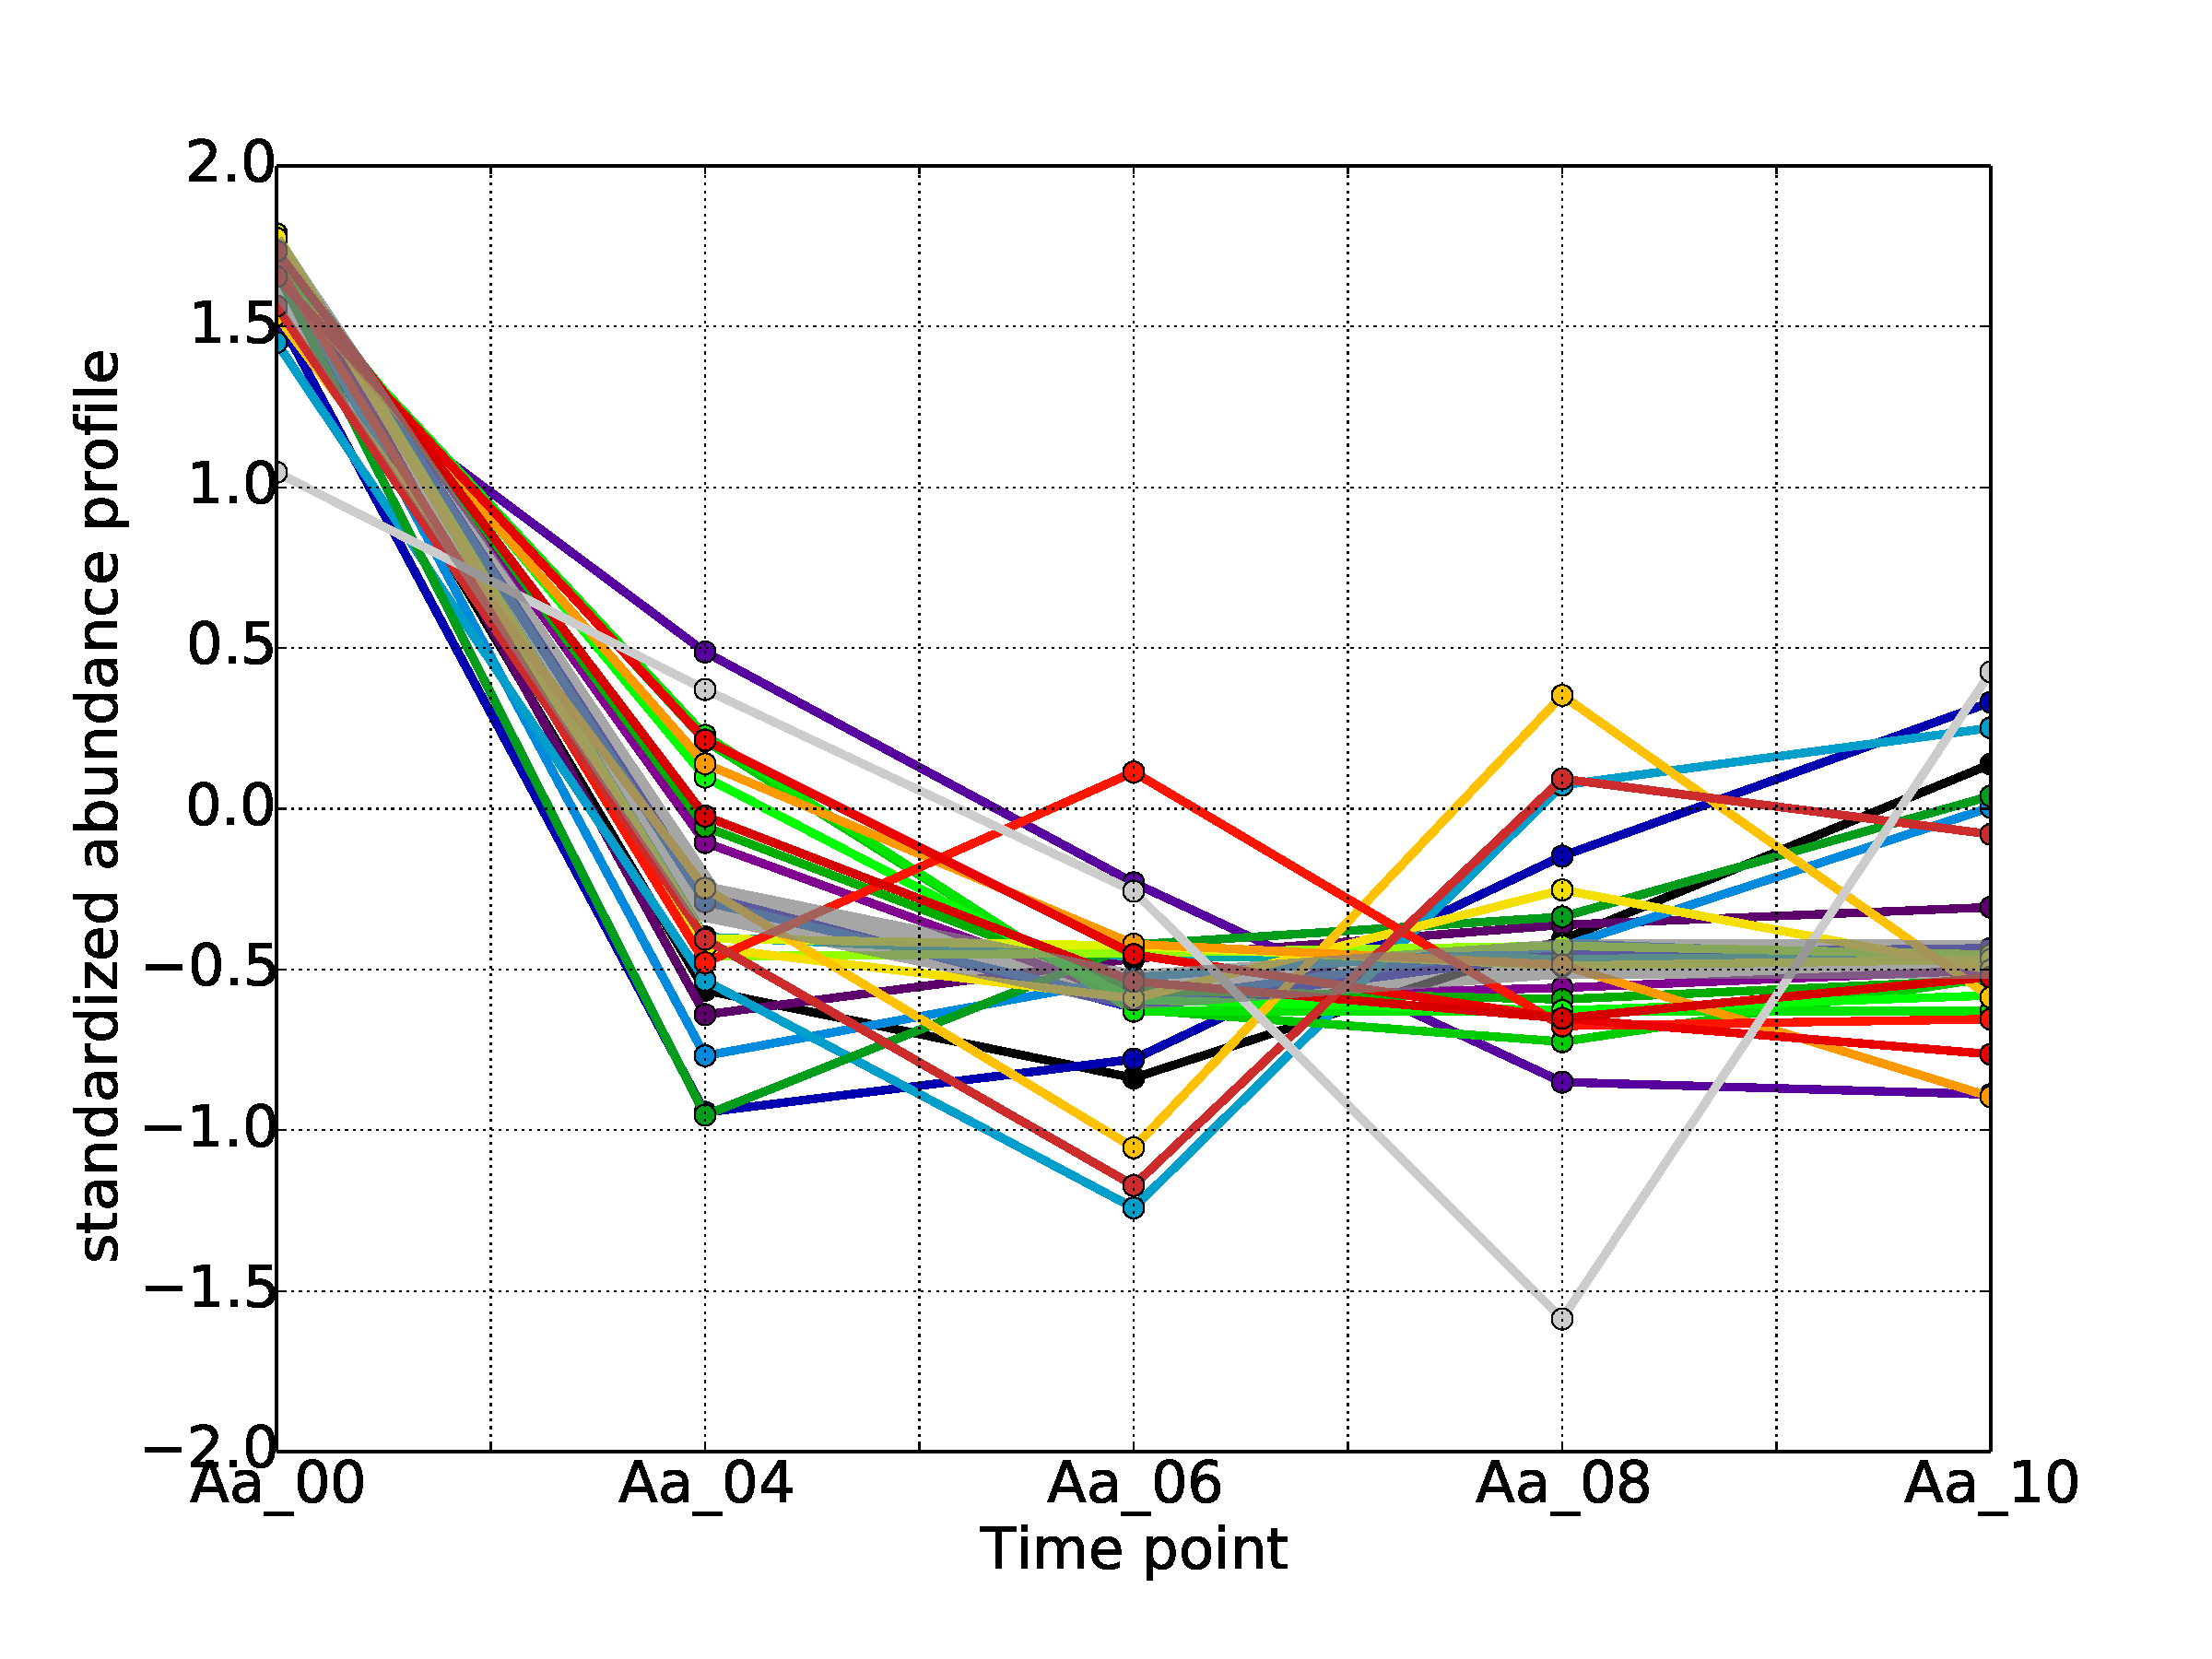
\includegraphics[width=.5\linewidth]{figures/figs/ecr_and_insects_ptci_20130918_orthodb7/downAfter4_gene_profiles_from_cummerbund/Aa_downAfter4_cls6_Ag_target_FPKMs_vb_orthos.pdf}}
%
\subcaptionbox{\label{fig:cluster6-Ag}}
{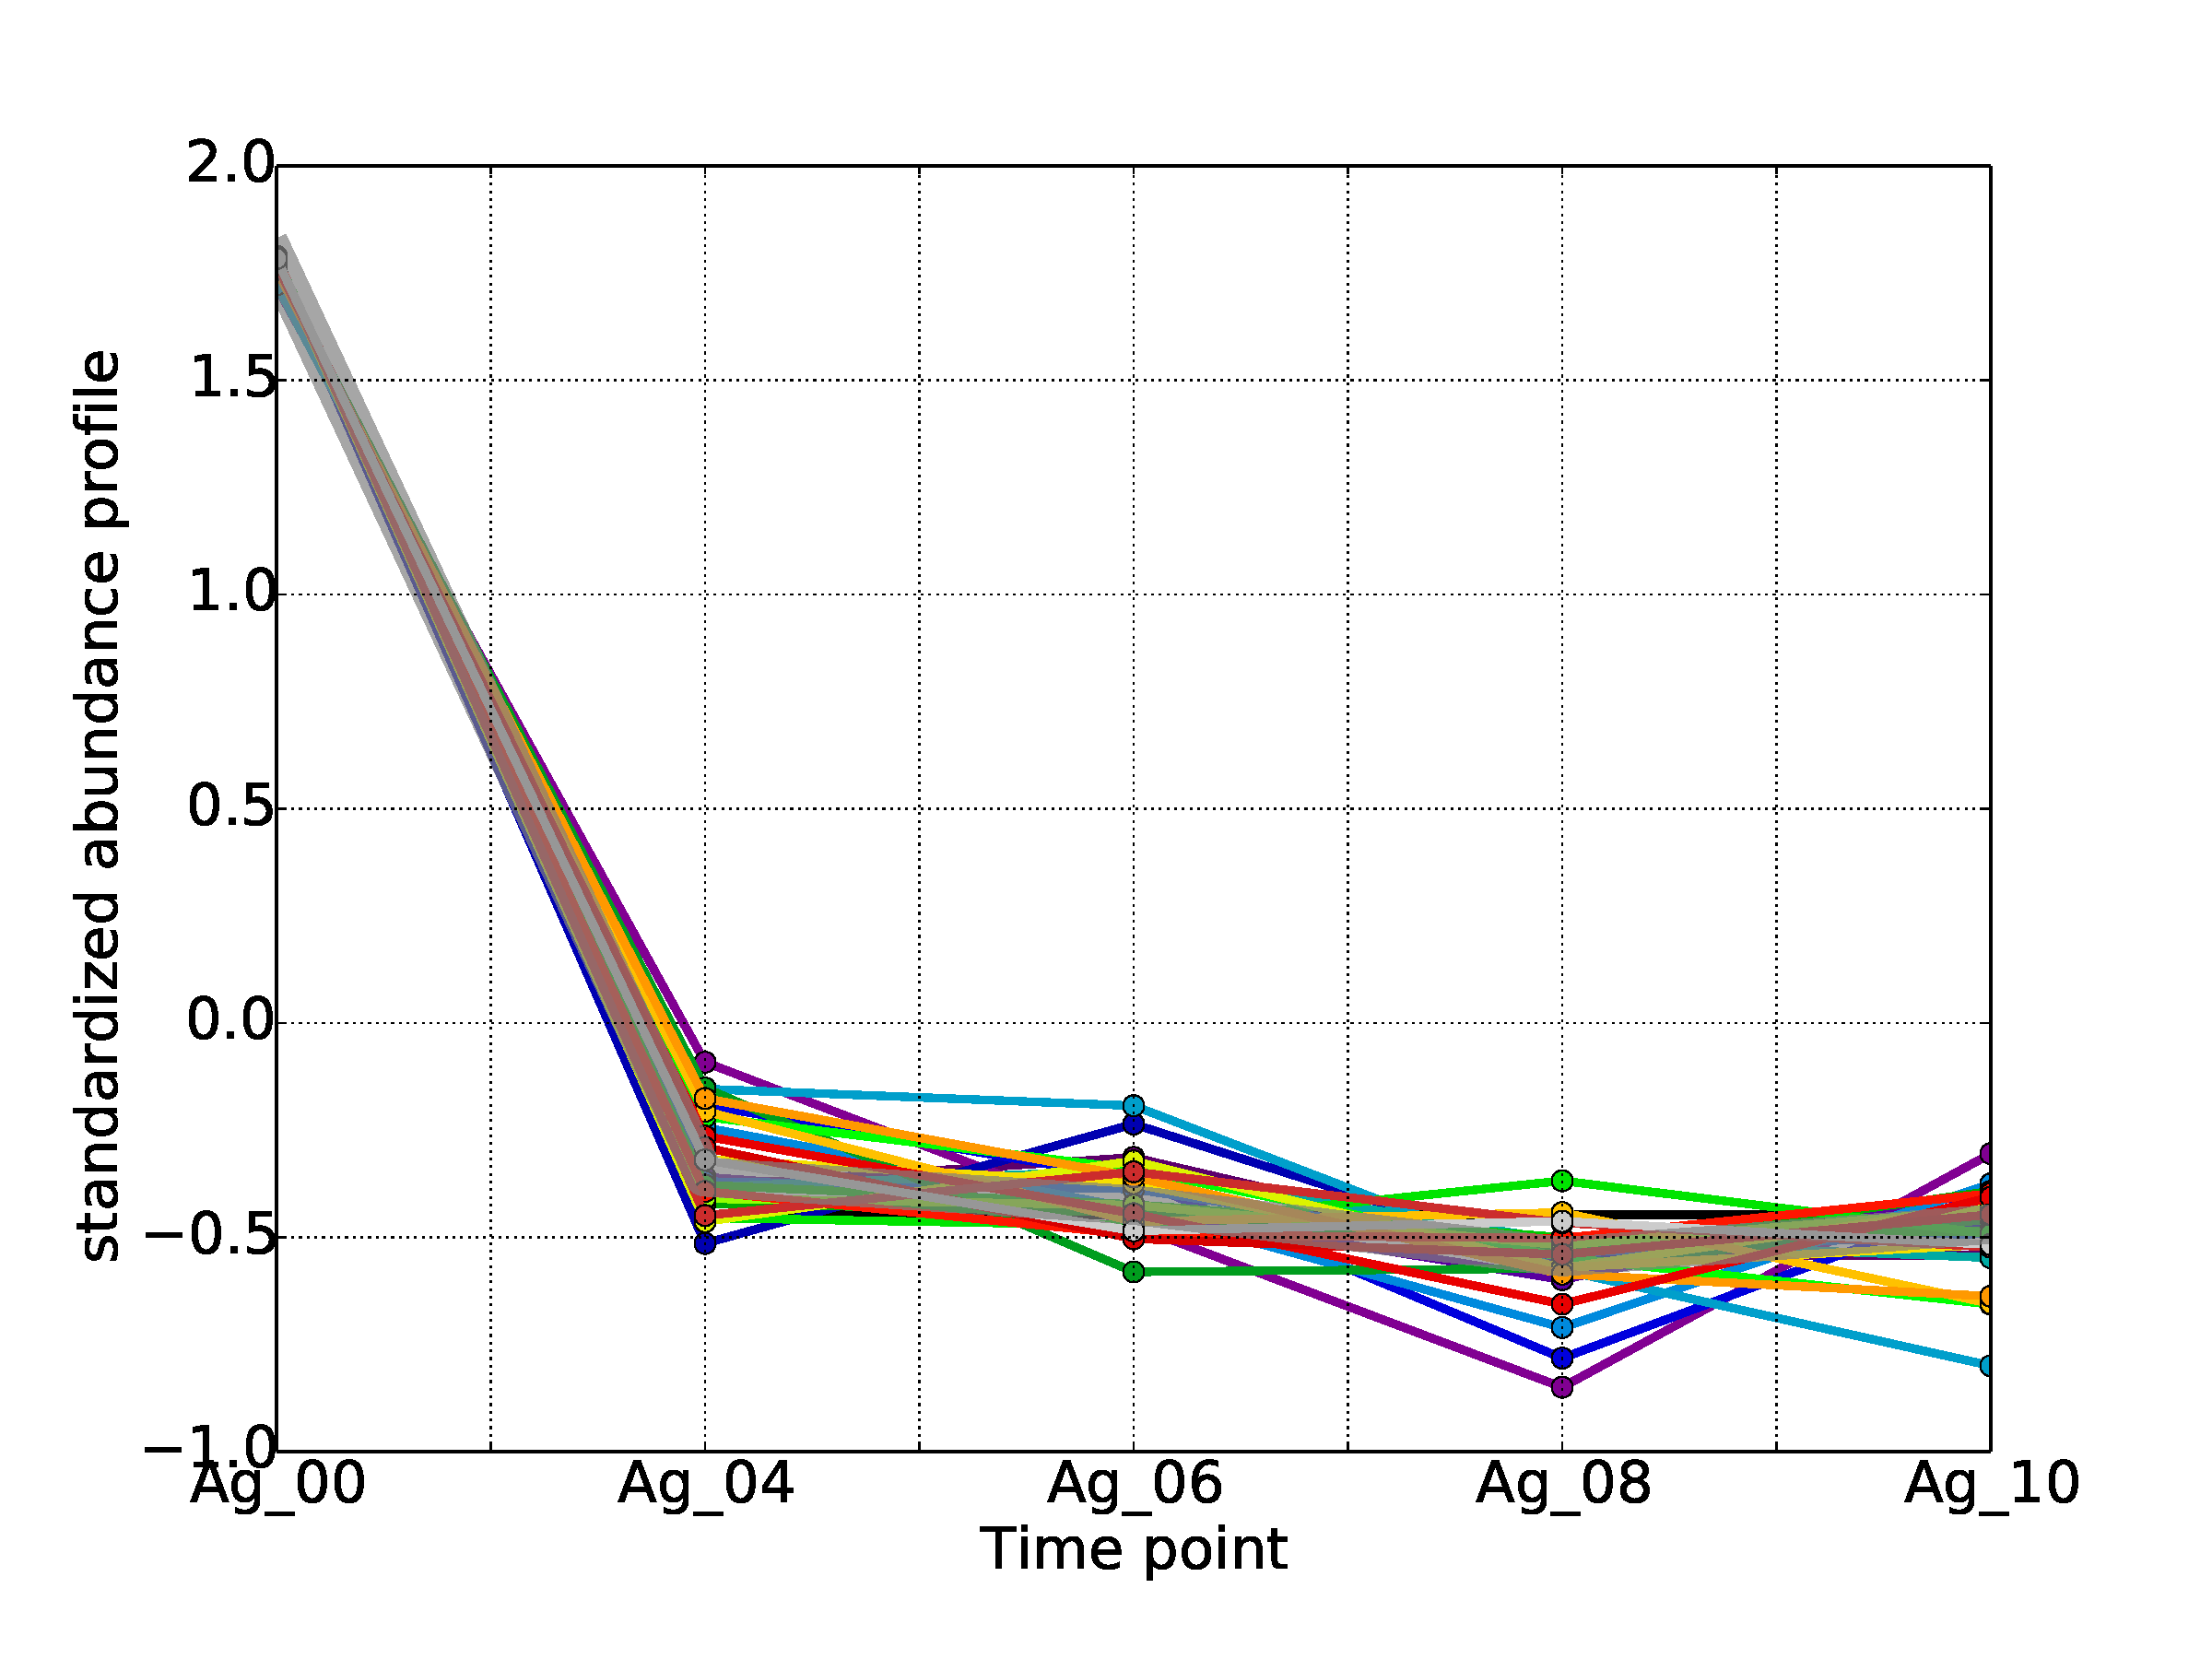
\includegraphics[width=.5\linewidth]{figures/figs/ecr_and_insects_ptci_20130918_orthodb7/downAfter4_gene_profiles_from_cummerbund/Ag_downAfter4_cls6_Ag_target_FPKMs_vb_orthos.pdf}}
%
\subcaptionbox{\label{fig:cluster6-Cq}}
{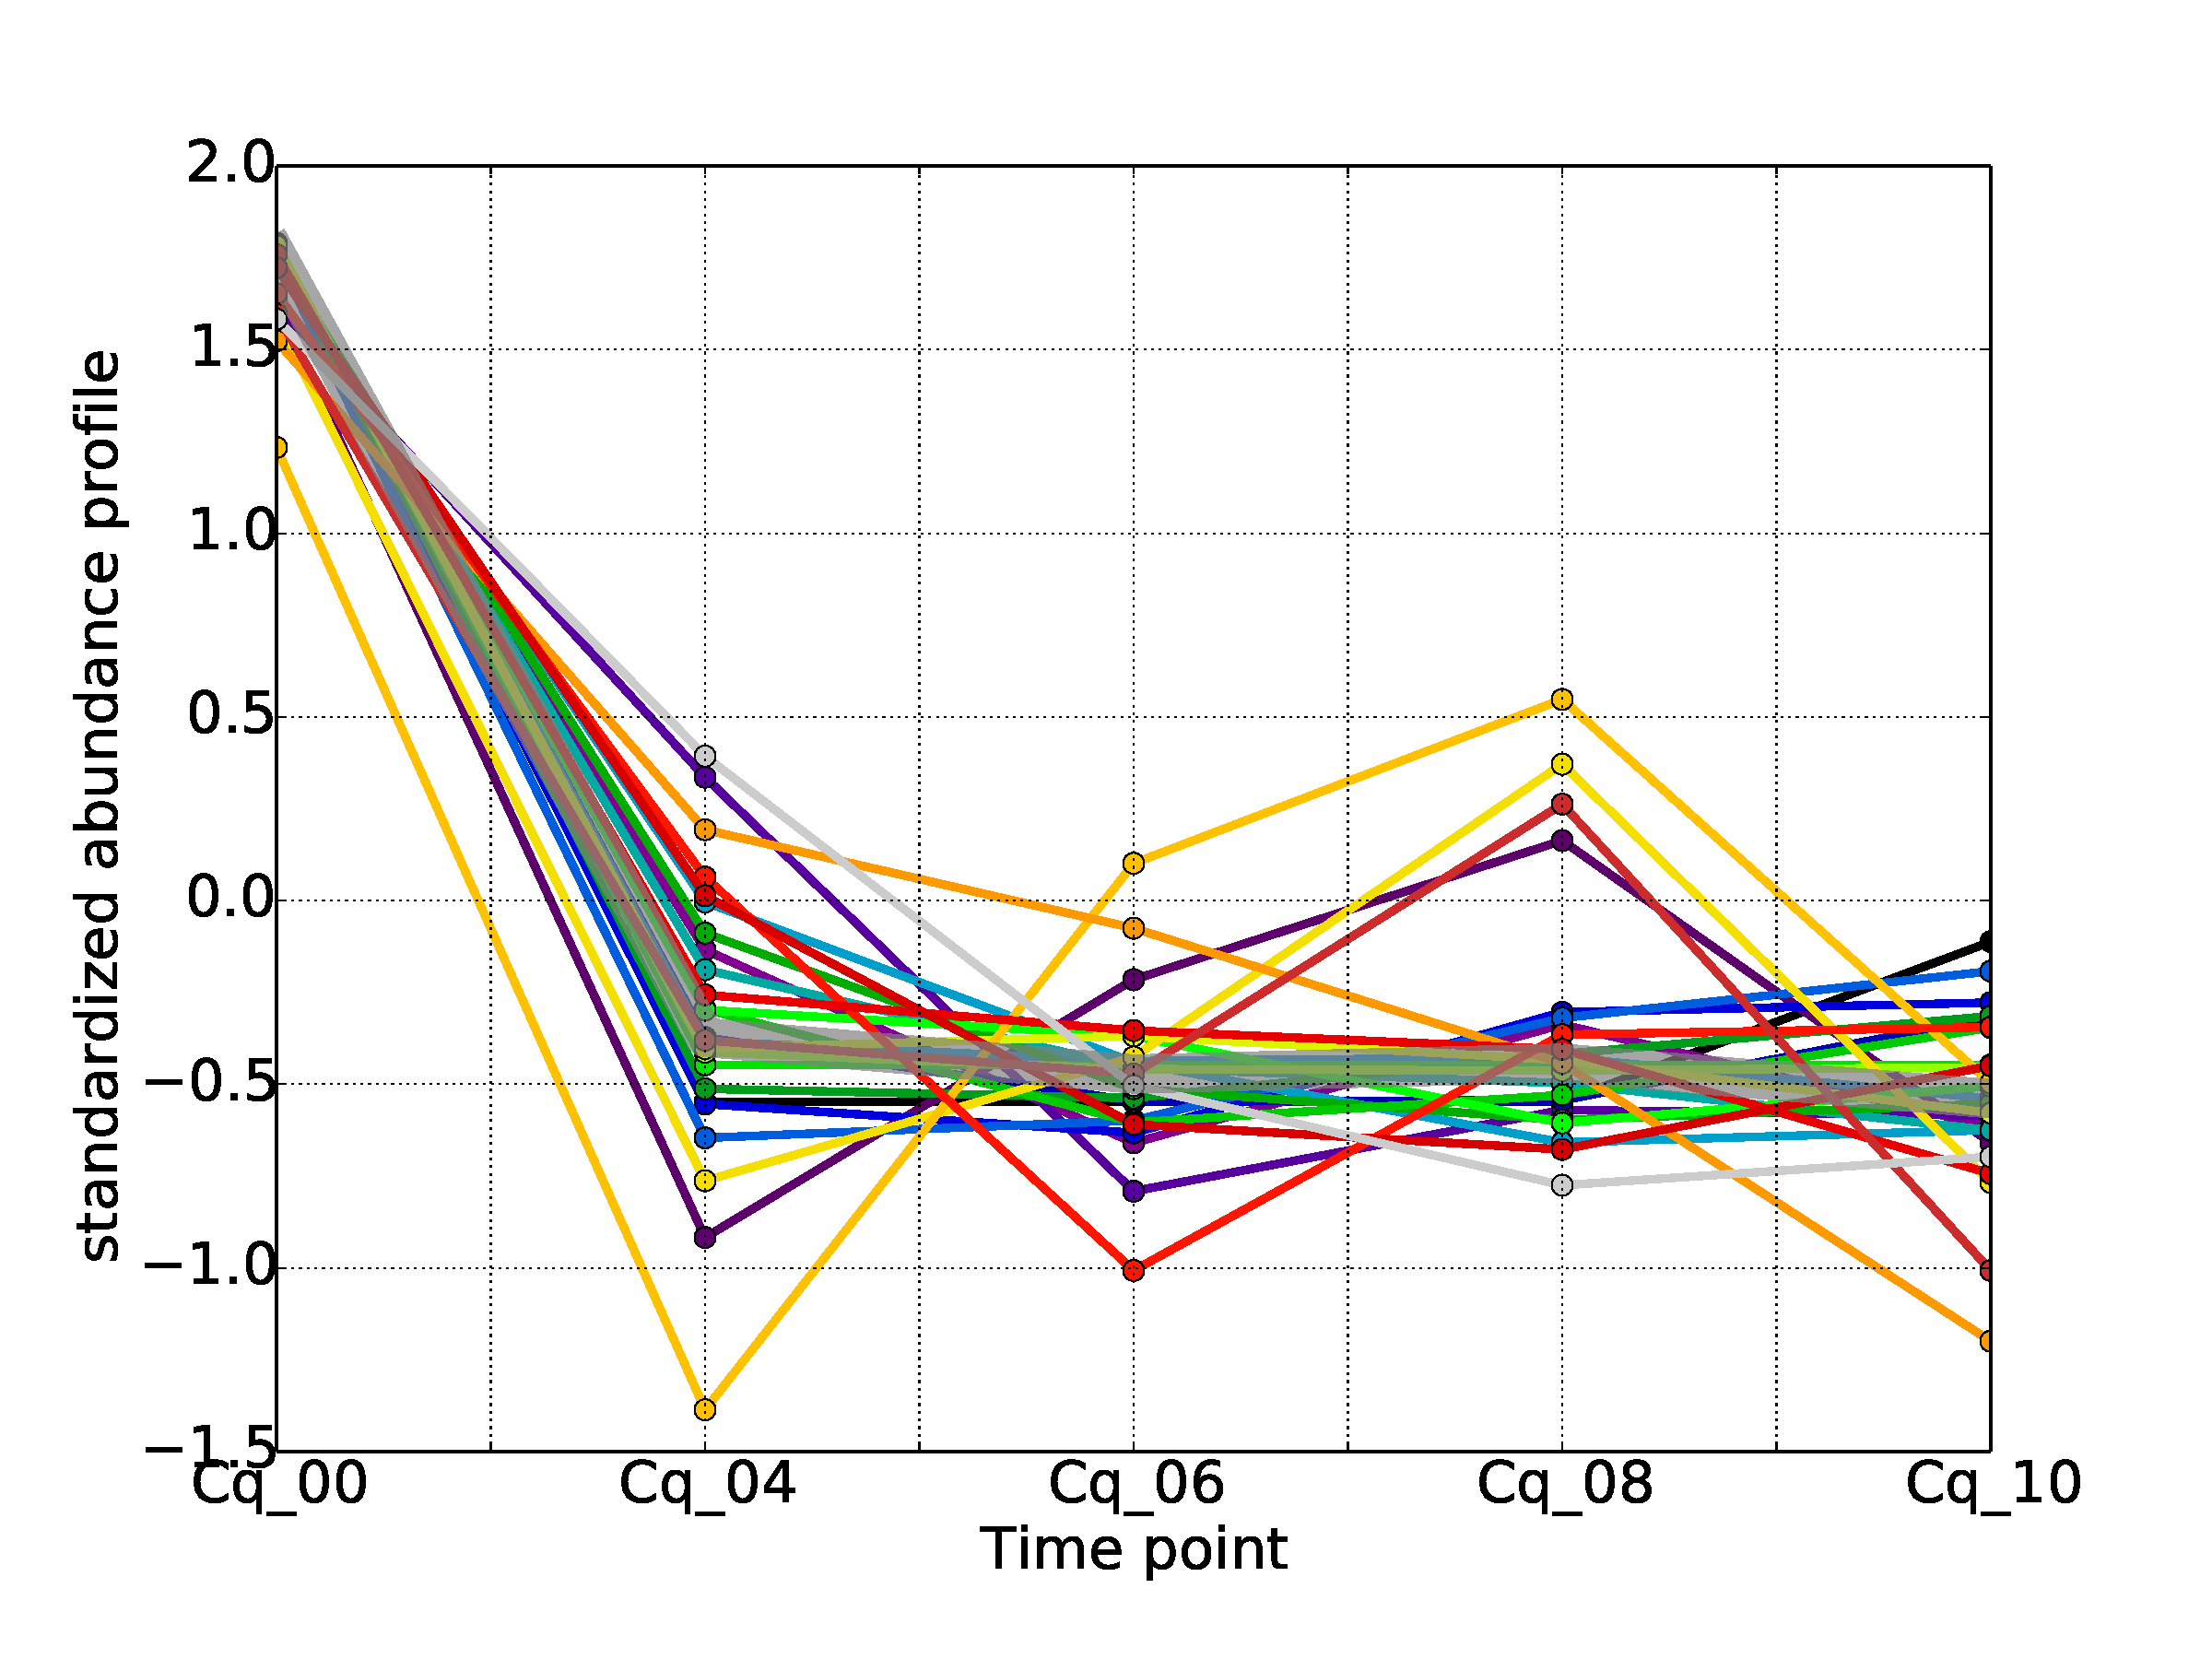
\includegraphics[width=.5\linewidth]{figures/figs/ecr_and_insects_ptci_20130918_orthodb7/downAfter4_gene_profiles_from_cummerbund/Cq_downAfter4_cls6_Ag_target_FPKMs_vb_orthos.pdf}}
% 
\caption[Orthologs of cluster 6]{\sf \textbf{Orthologs of cluster 6 (down after 4h):}\\
The same color scheme is used for each species which means that orthologs are given the same color in all three panels.
The thick, transparent gray line represents the median \gls{mAP} for the panel.
\textbf{(A)} \Aa.
\textbf{(B)} \Ag.
\textbf{(C)} \Cq.
}\label{fig:cluster6}
\end{figure}
\begin{figure}[p]
% 
\subcaptionbox{\label{fig:cluster16-Aa}}
{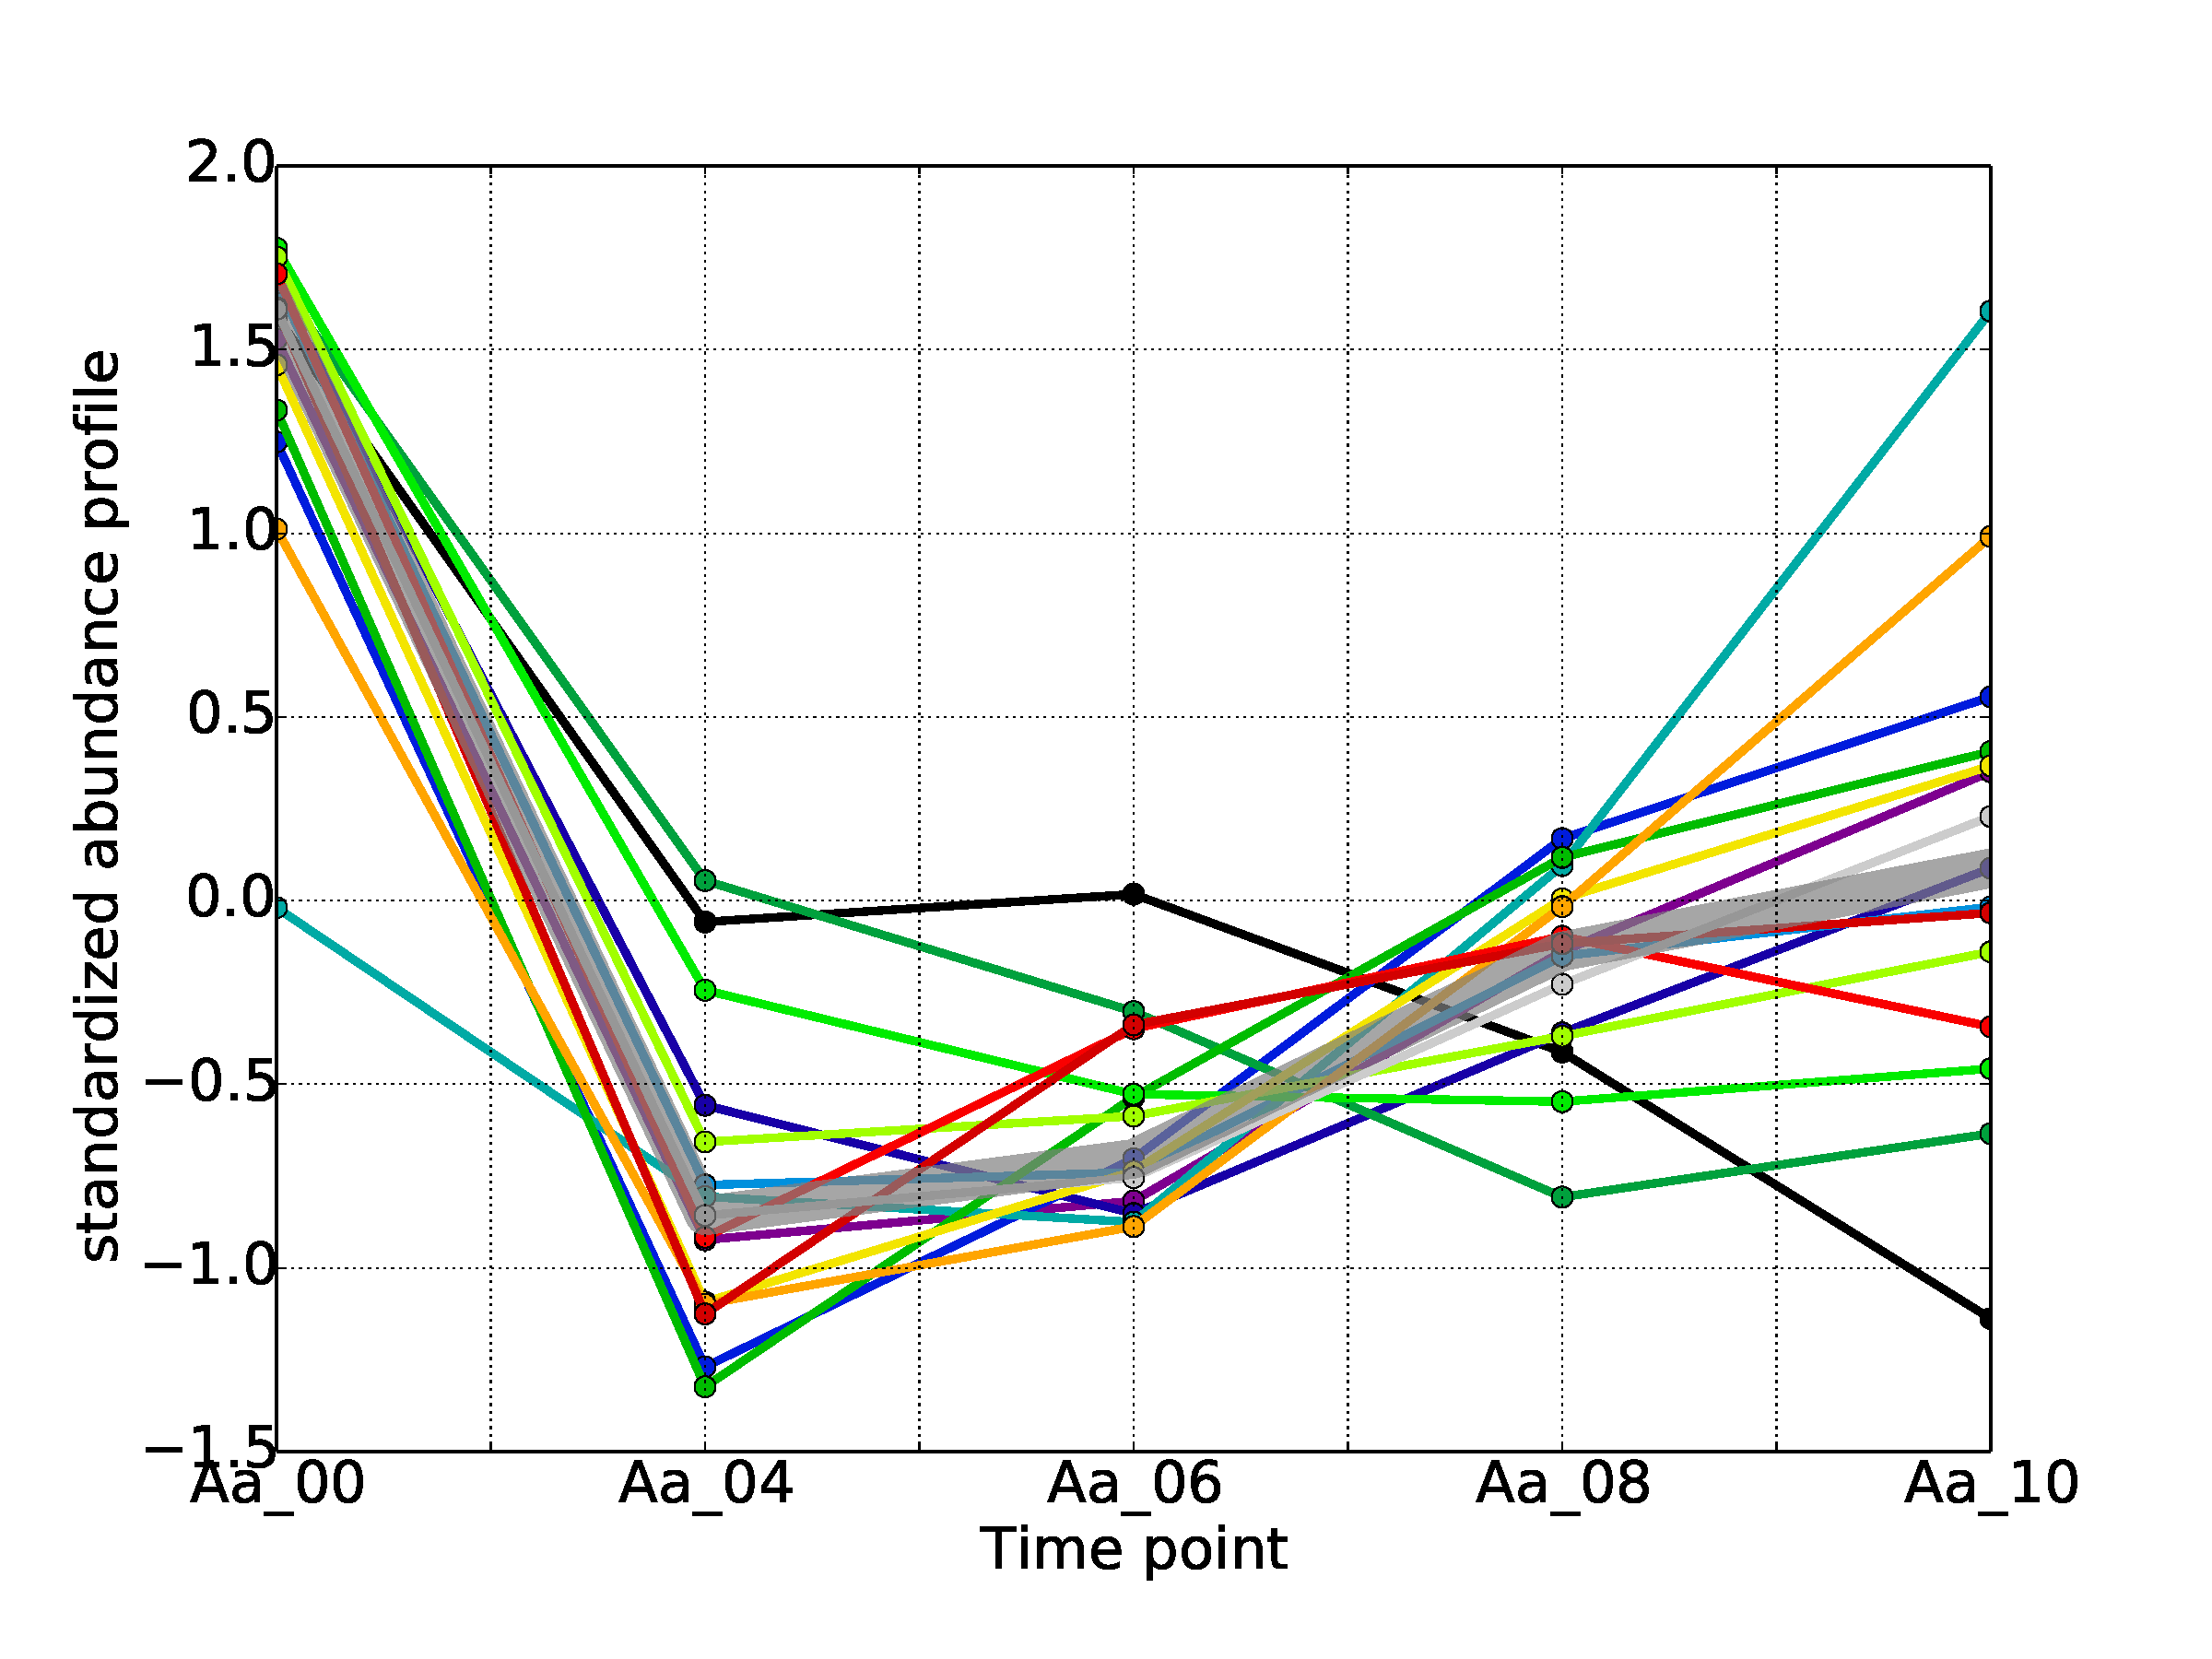
\includegraphics[width=.5\linewidth]{figures/figs/ecr_and_insects_ptci_20130918_orthodb7/downAt4_gene_profiles_from_cummerbund/Aa_downAt4_cls16_Ag_target_FPKMs_vb_orthos.pdf}}
%
\subcaptionbox{\label{fig:cluster16-Ag}}
{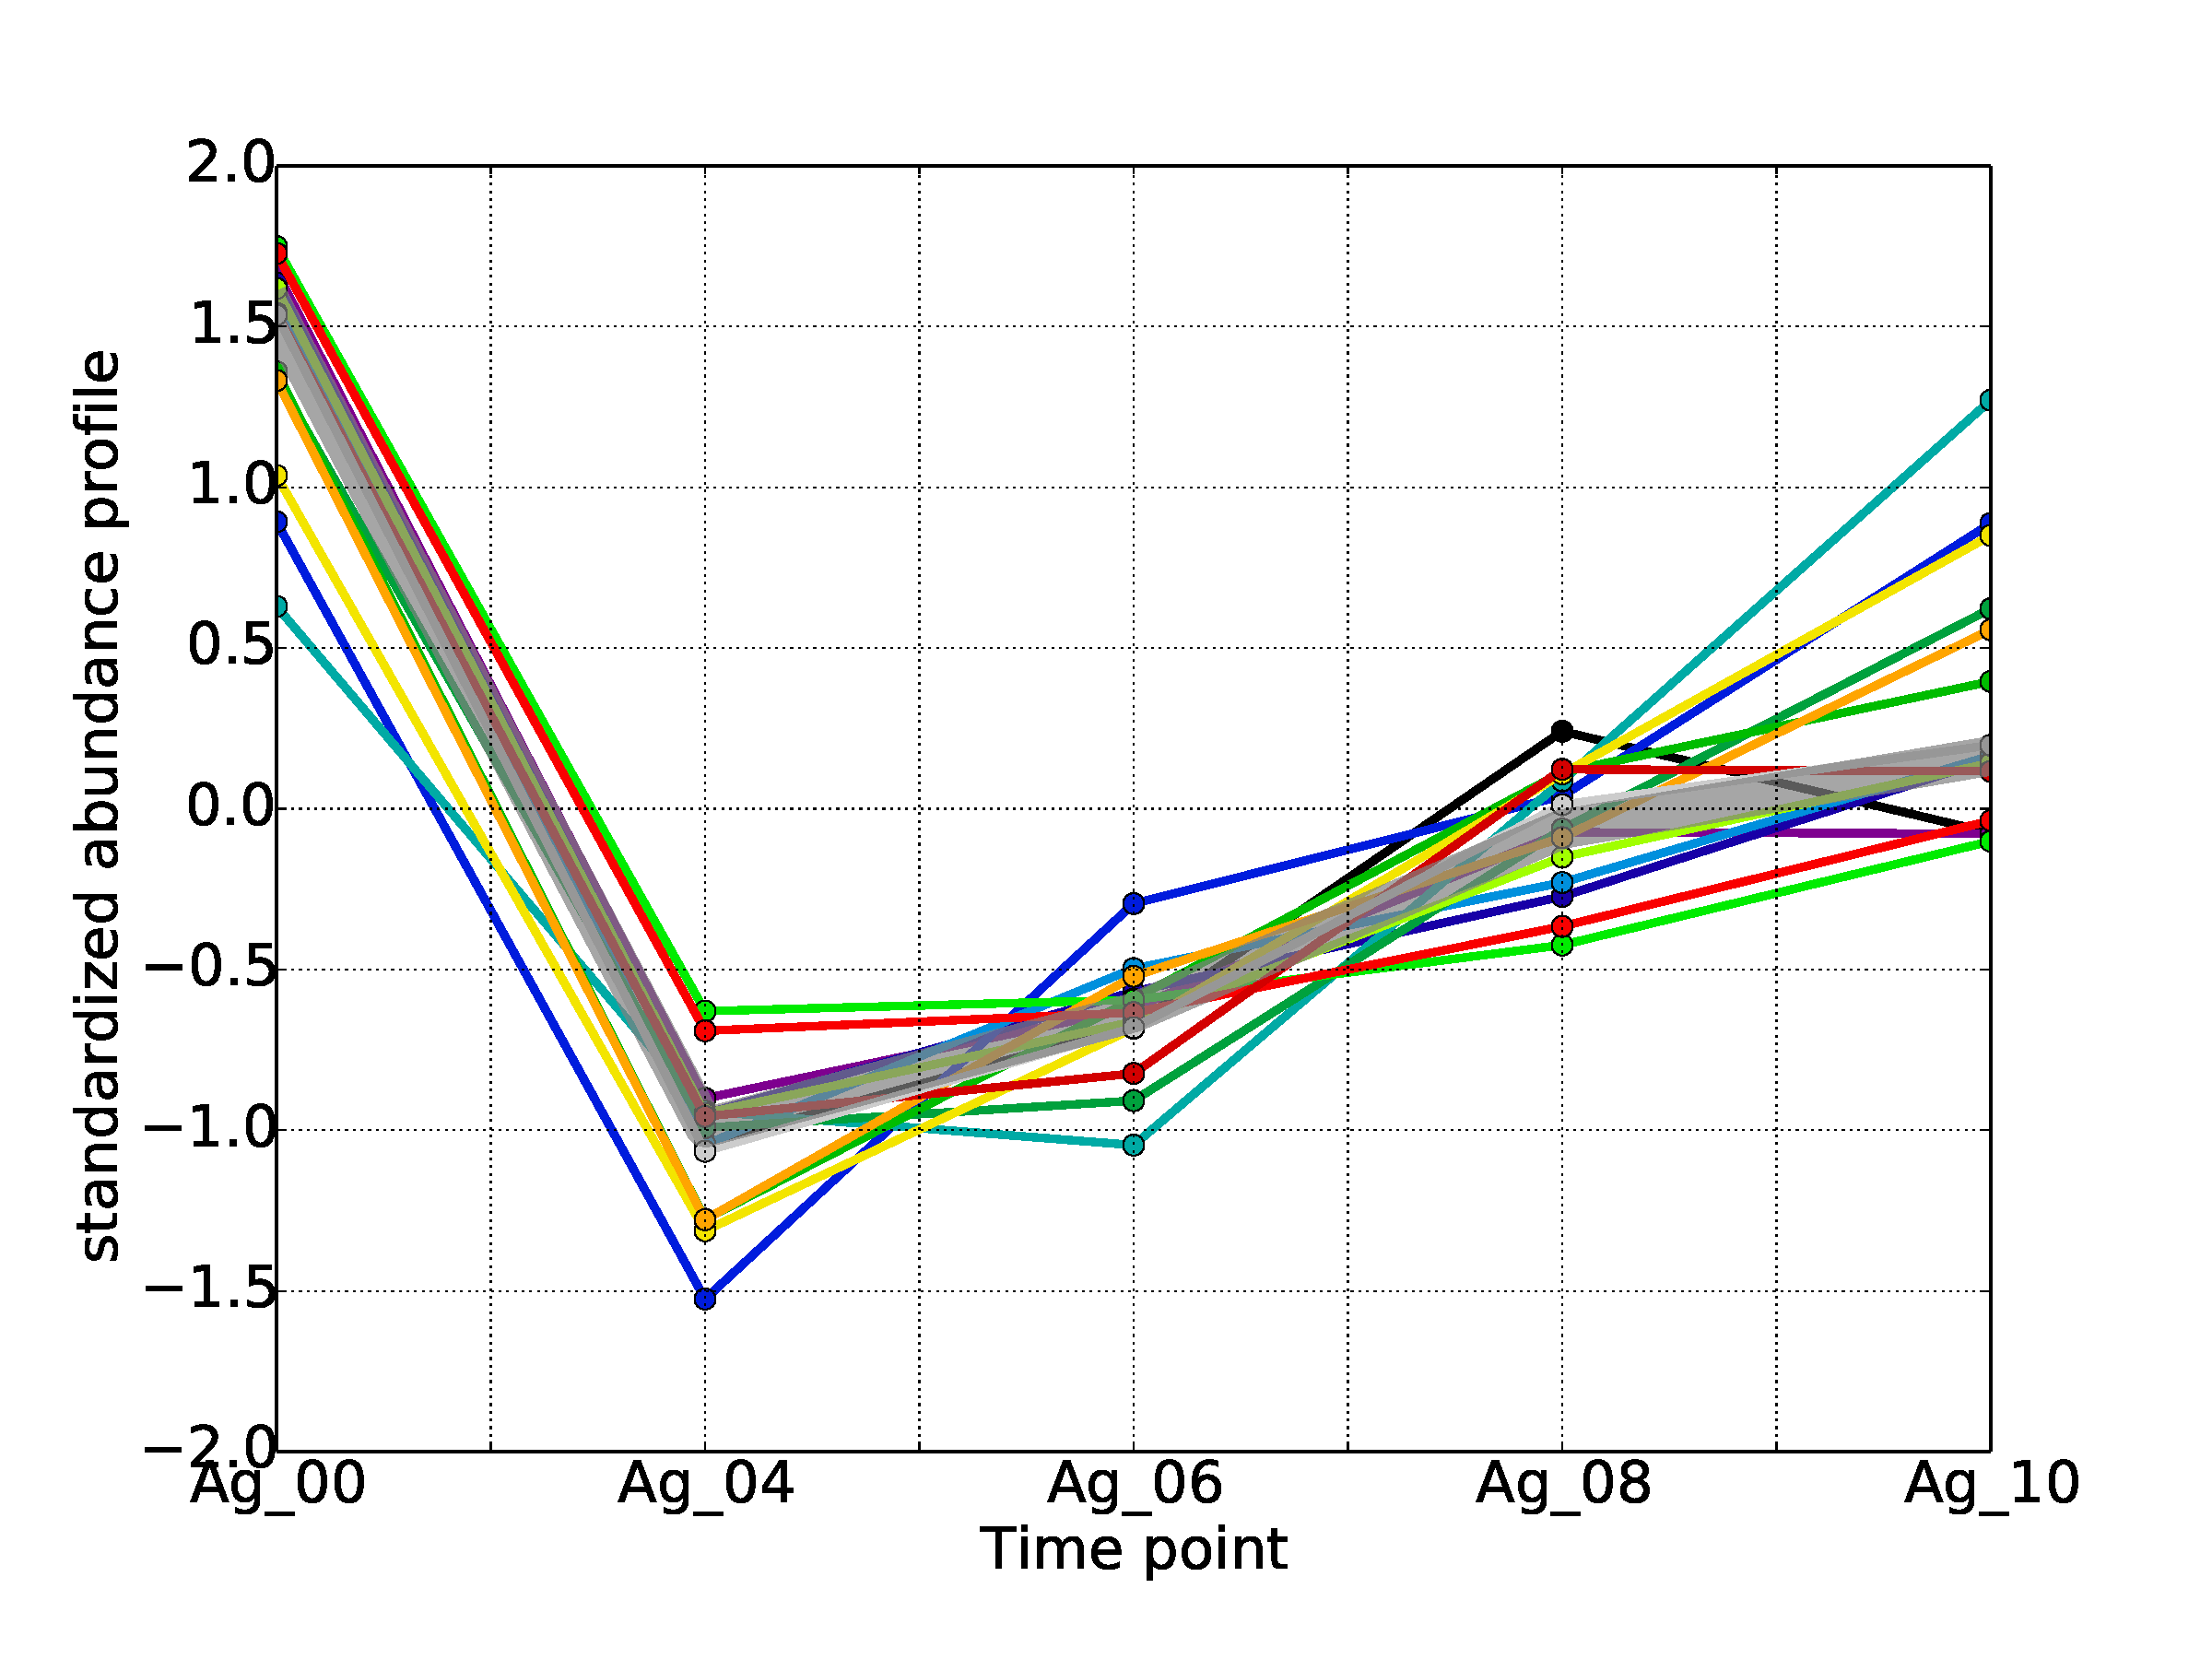
\includegraphics[width=.5\linewidth]{figures/figs/ecr_and_insects_ptci_20130918_orthodb7/downAt4_gene_profiles_from_cummerbund/Ag_downAt4_cls16_Ag_target_FPKMs_vb_orthos.pdf}}
%
\subcaptionbox{\label{fig:cluster16-Cq}}
{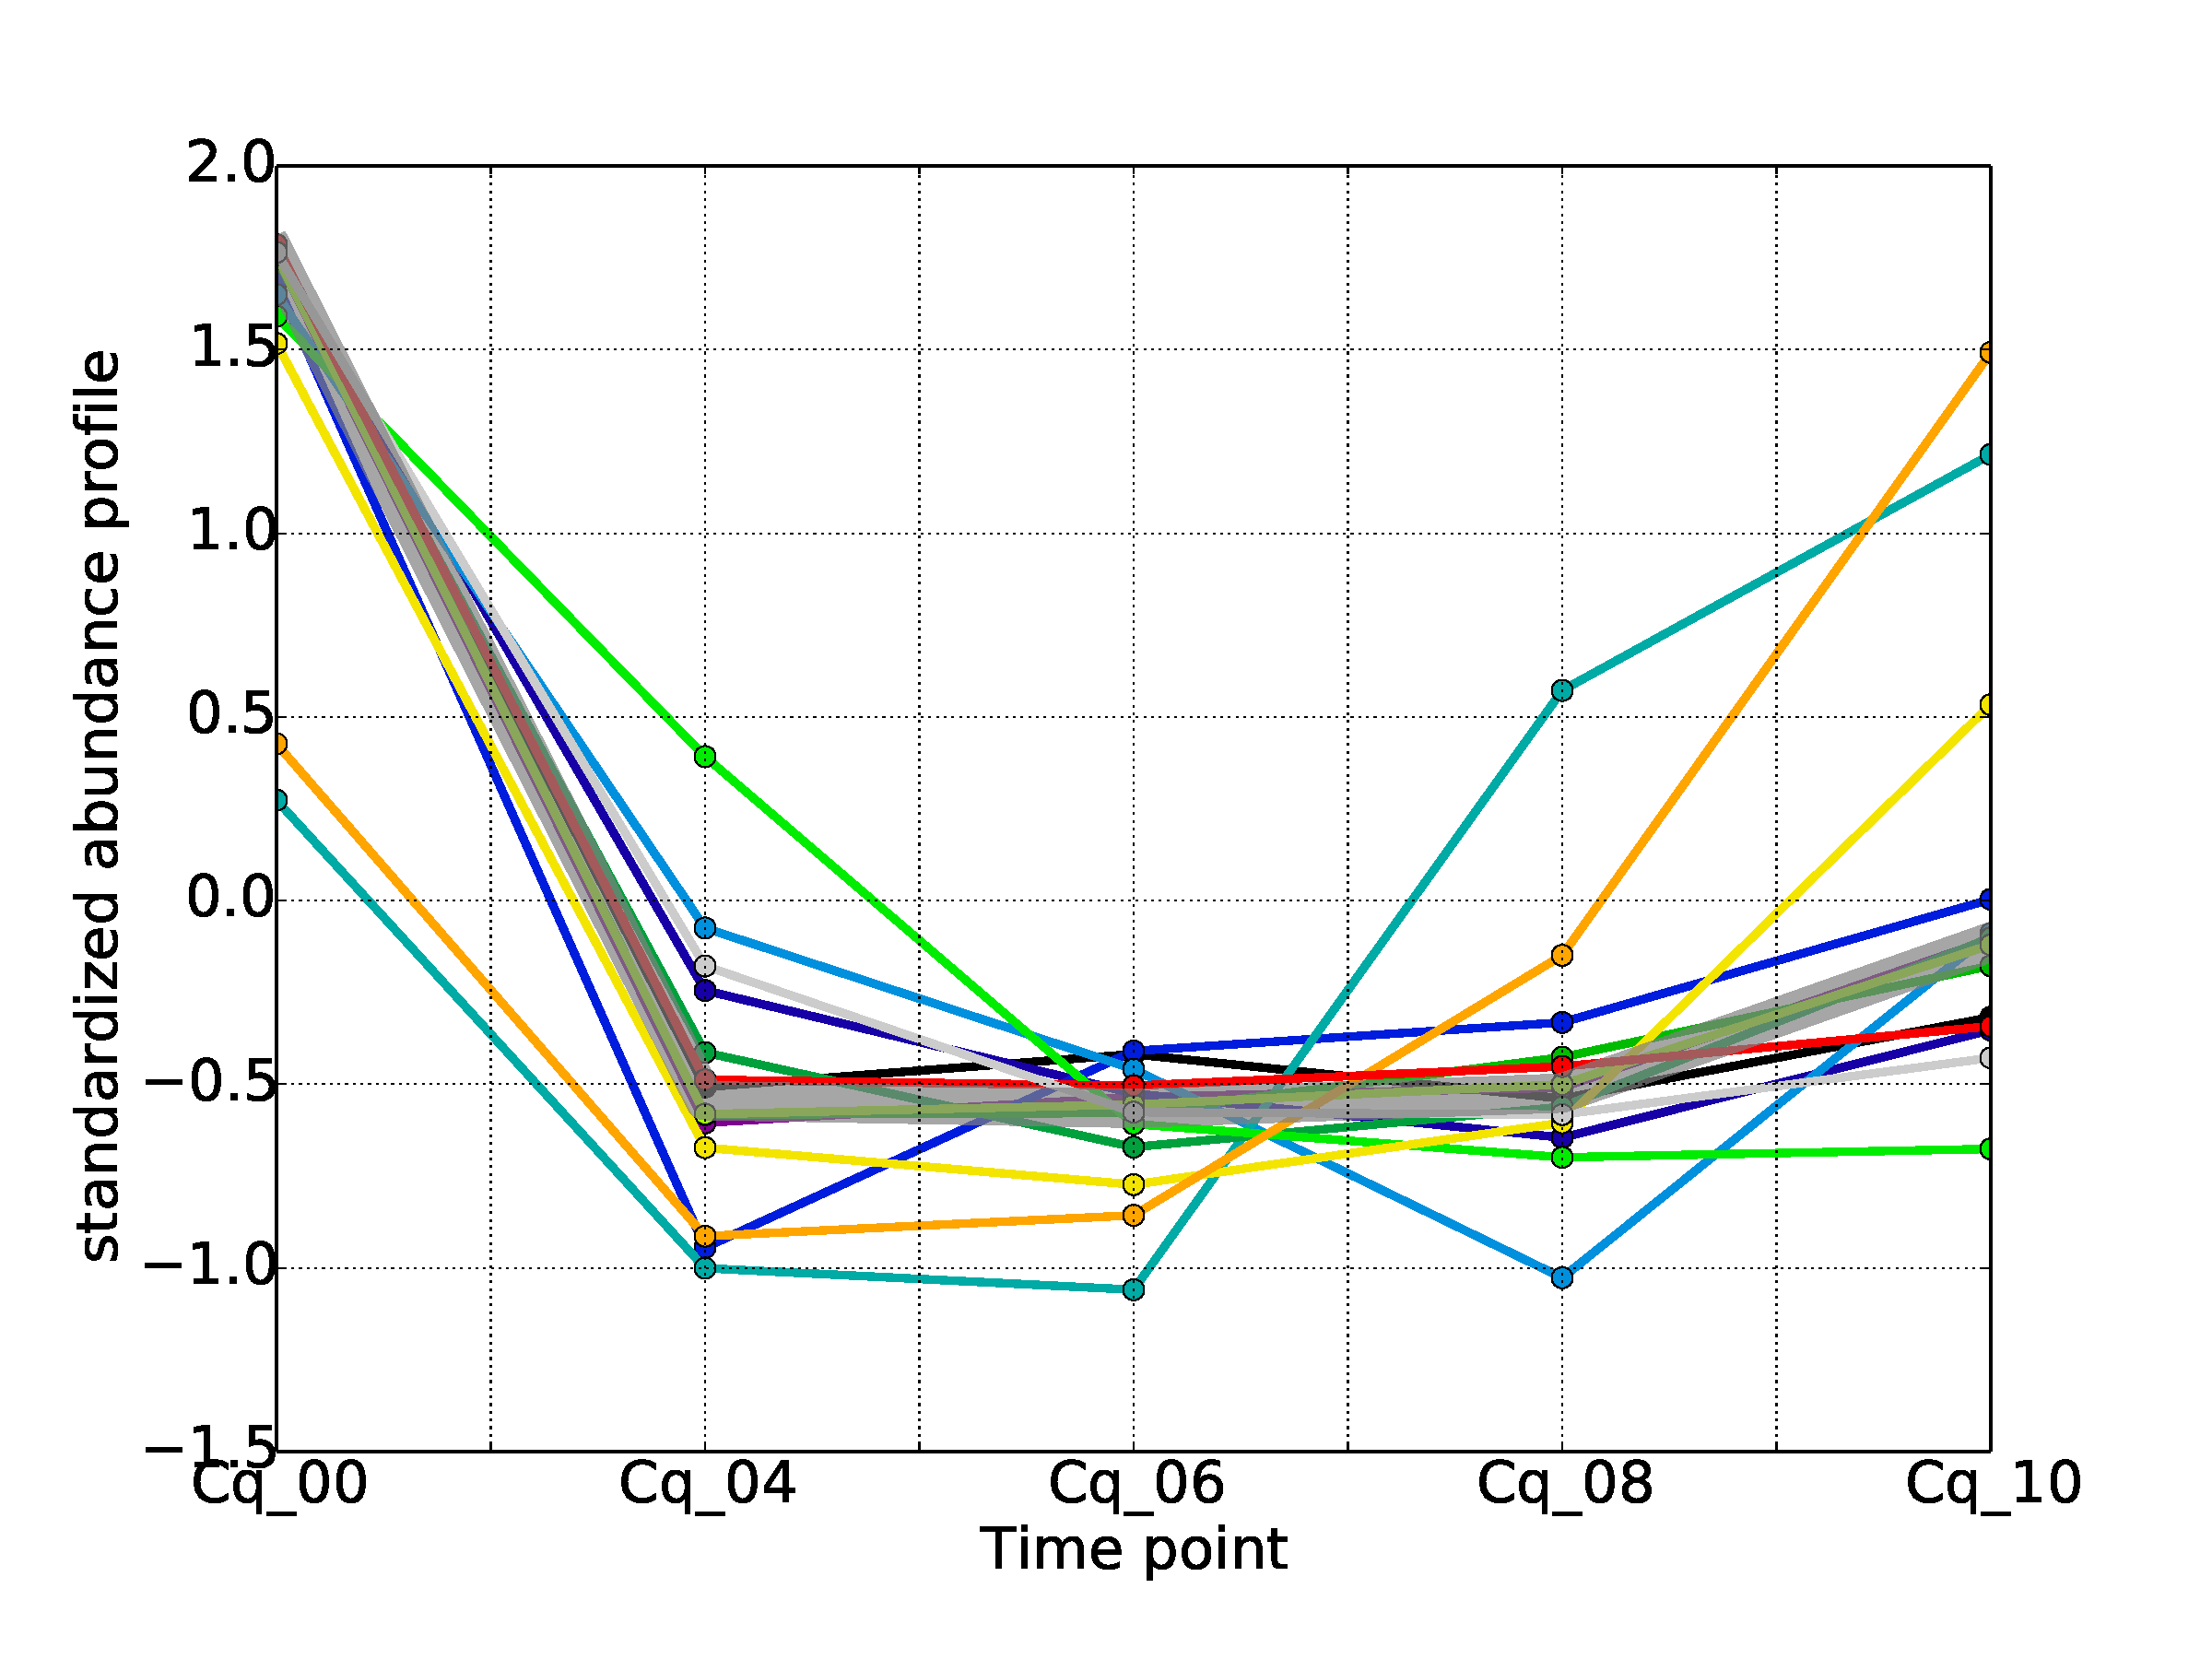
\includegraphics[width=.5\linewidth]{figures/figs/ecr_and_insects_ptci_20130918_orthodb7/downAt4_gene_profiles_from_cummerbund/Cq_downAt4_cls16_Ag_target_FPKMs_vb_orthos.pdf}}
% 
\caption[Orthologs of cluster 16]{\sf \textbf{Orthologs of cluster 16 (down at 4h):}\\
The same color scheme is used for each species which means that orthologs are given the same color in all three panels.
The thick, transparent gray line represents the median \gls{mAP} for the panel.
\textbf{(A)} \Aa.
\textbf{(B)} \Ag.
\textbf{(C)} \Cq.
}\label{fig:cluster16}
\end{figure}
\begin{figure}[p]
% 
\subcaptionbox{\label{fig:cluster22-Aa}}
{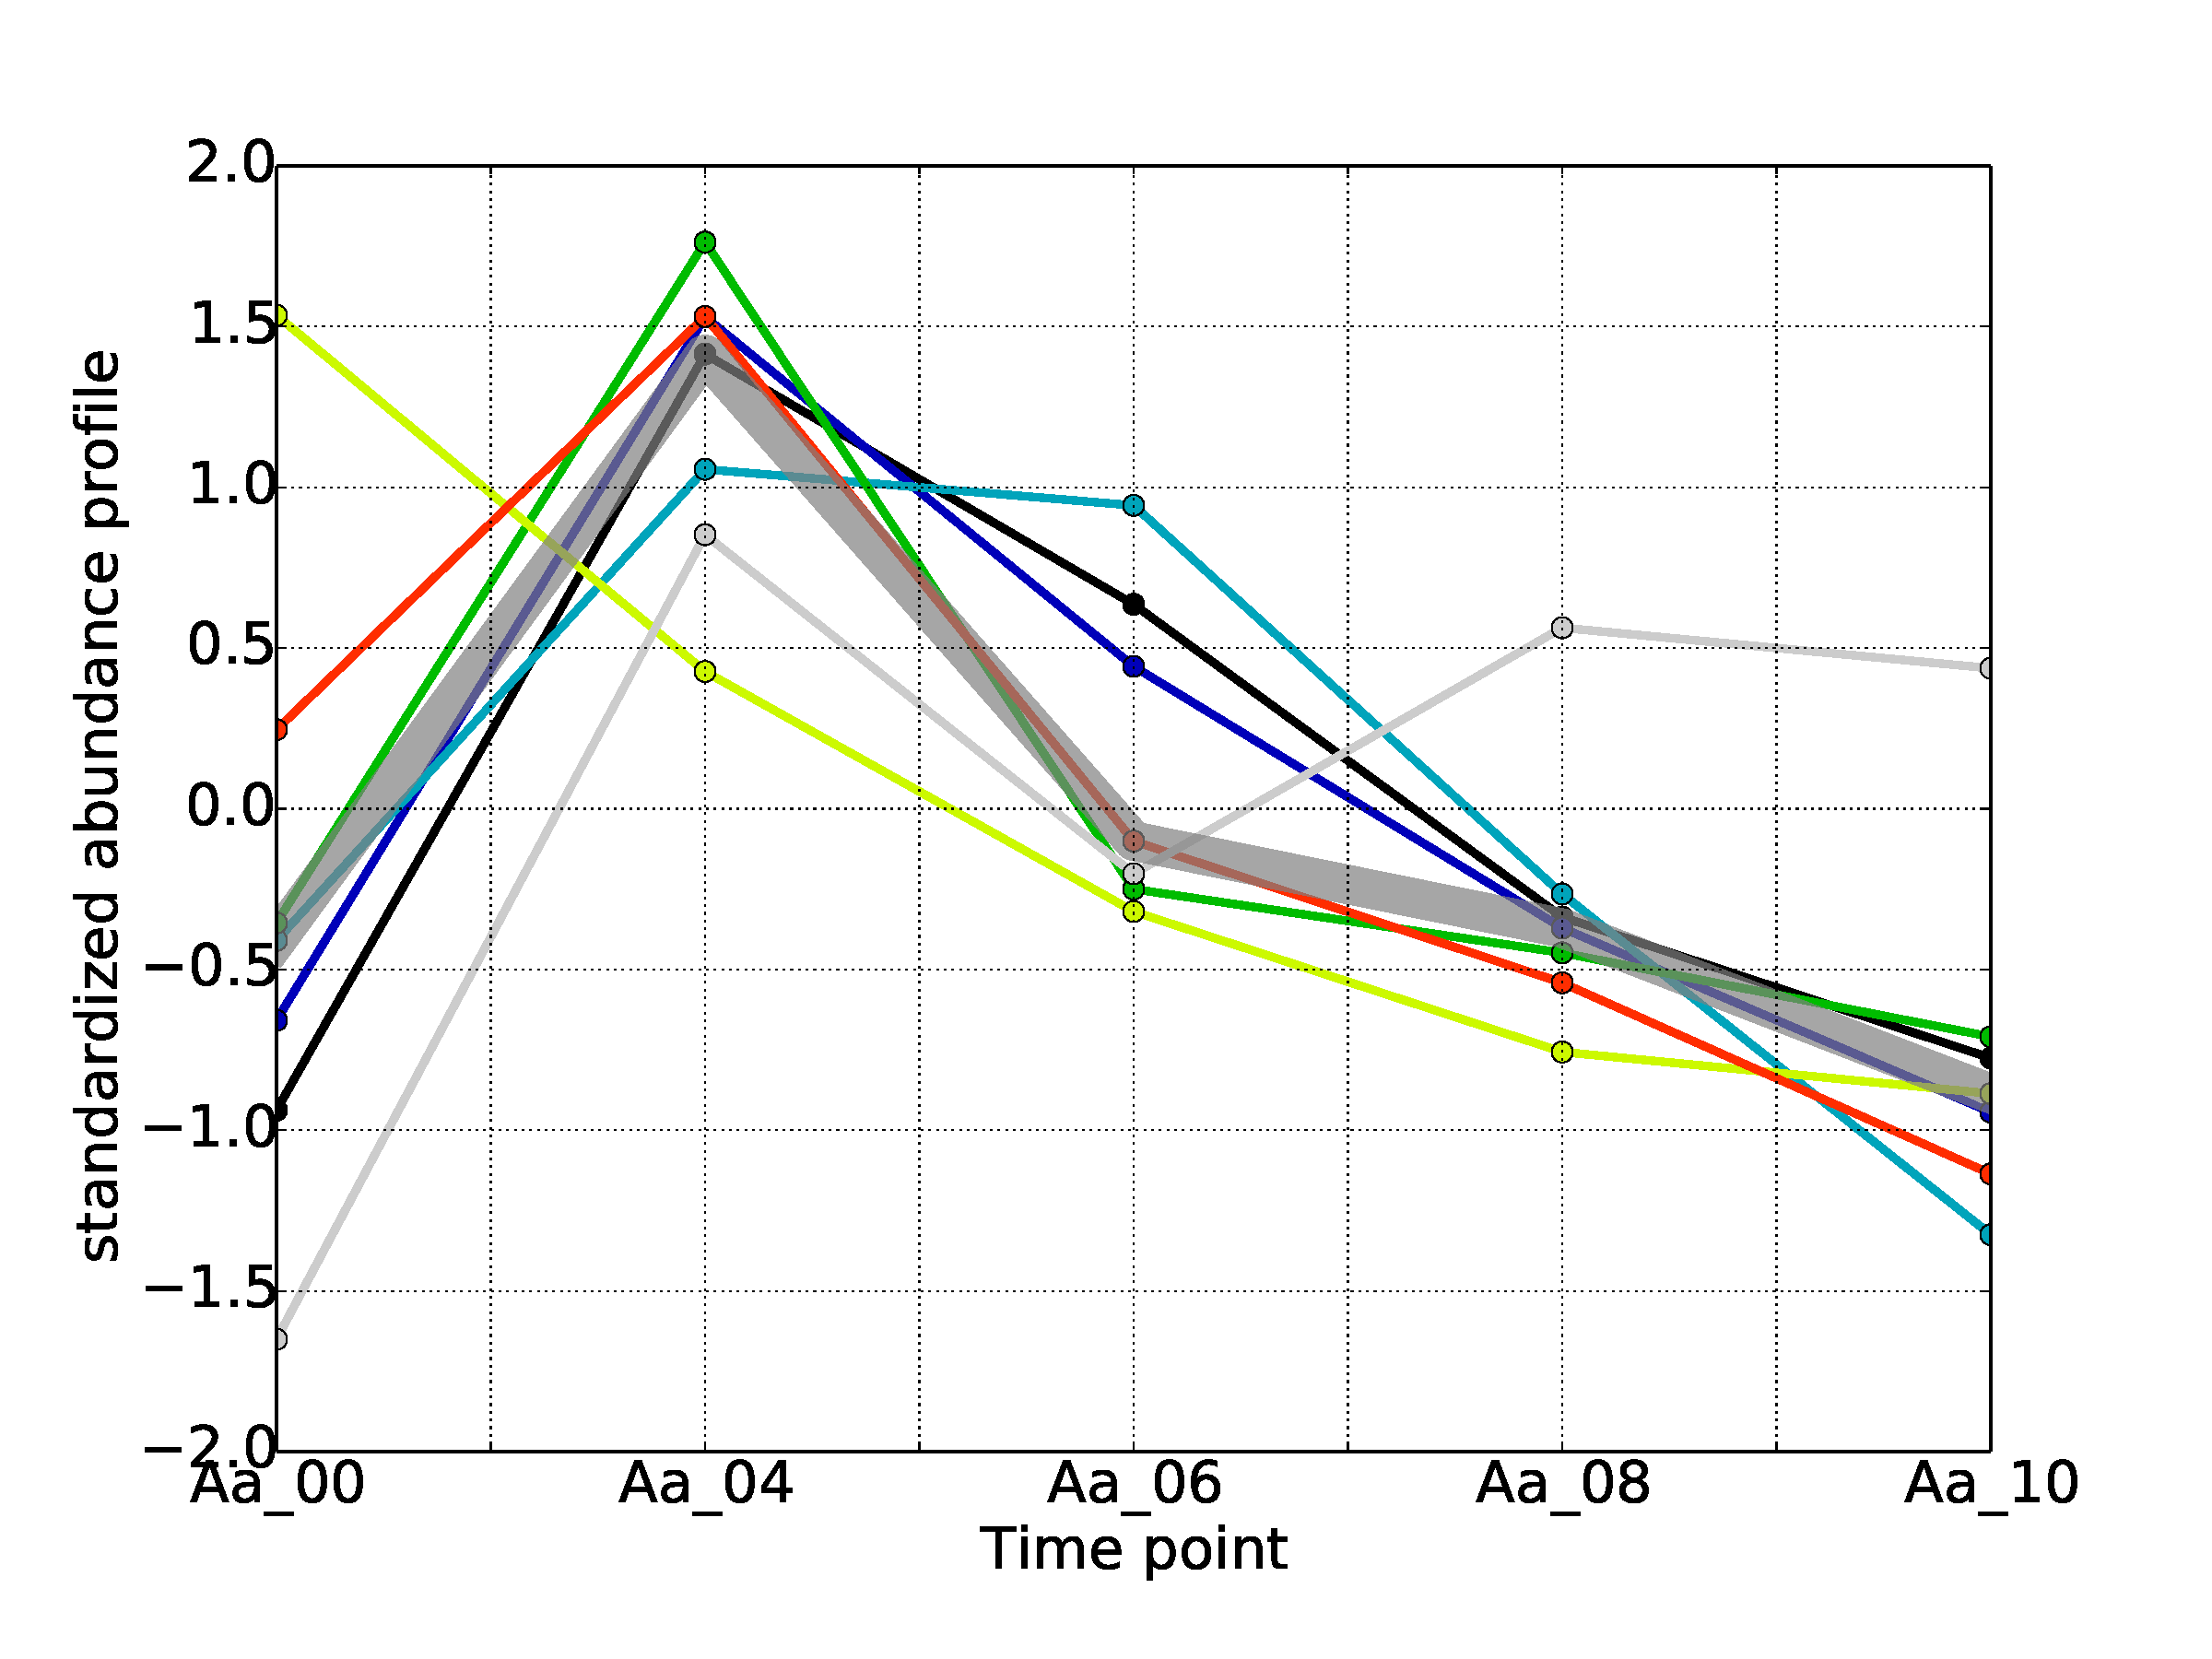
\includegraphics[width=.5\linewidth]{figures/figs/ecr_and_insects_ptci_20130918_orthodb7/upAt4_gene_profiles_from_cummerbund/Aa_upAt4_cls22_Ag_target_FPKMs_vb_orthos.pdf}}
%
\subcaptionbox{\label{fig:cluster22-Ag}}
{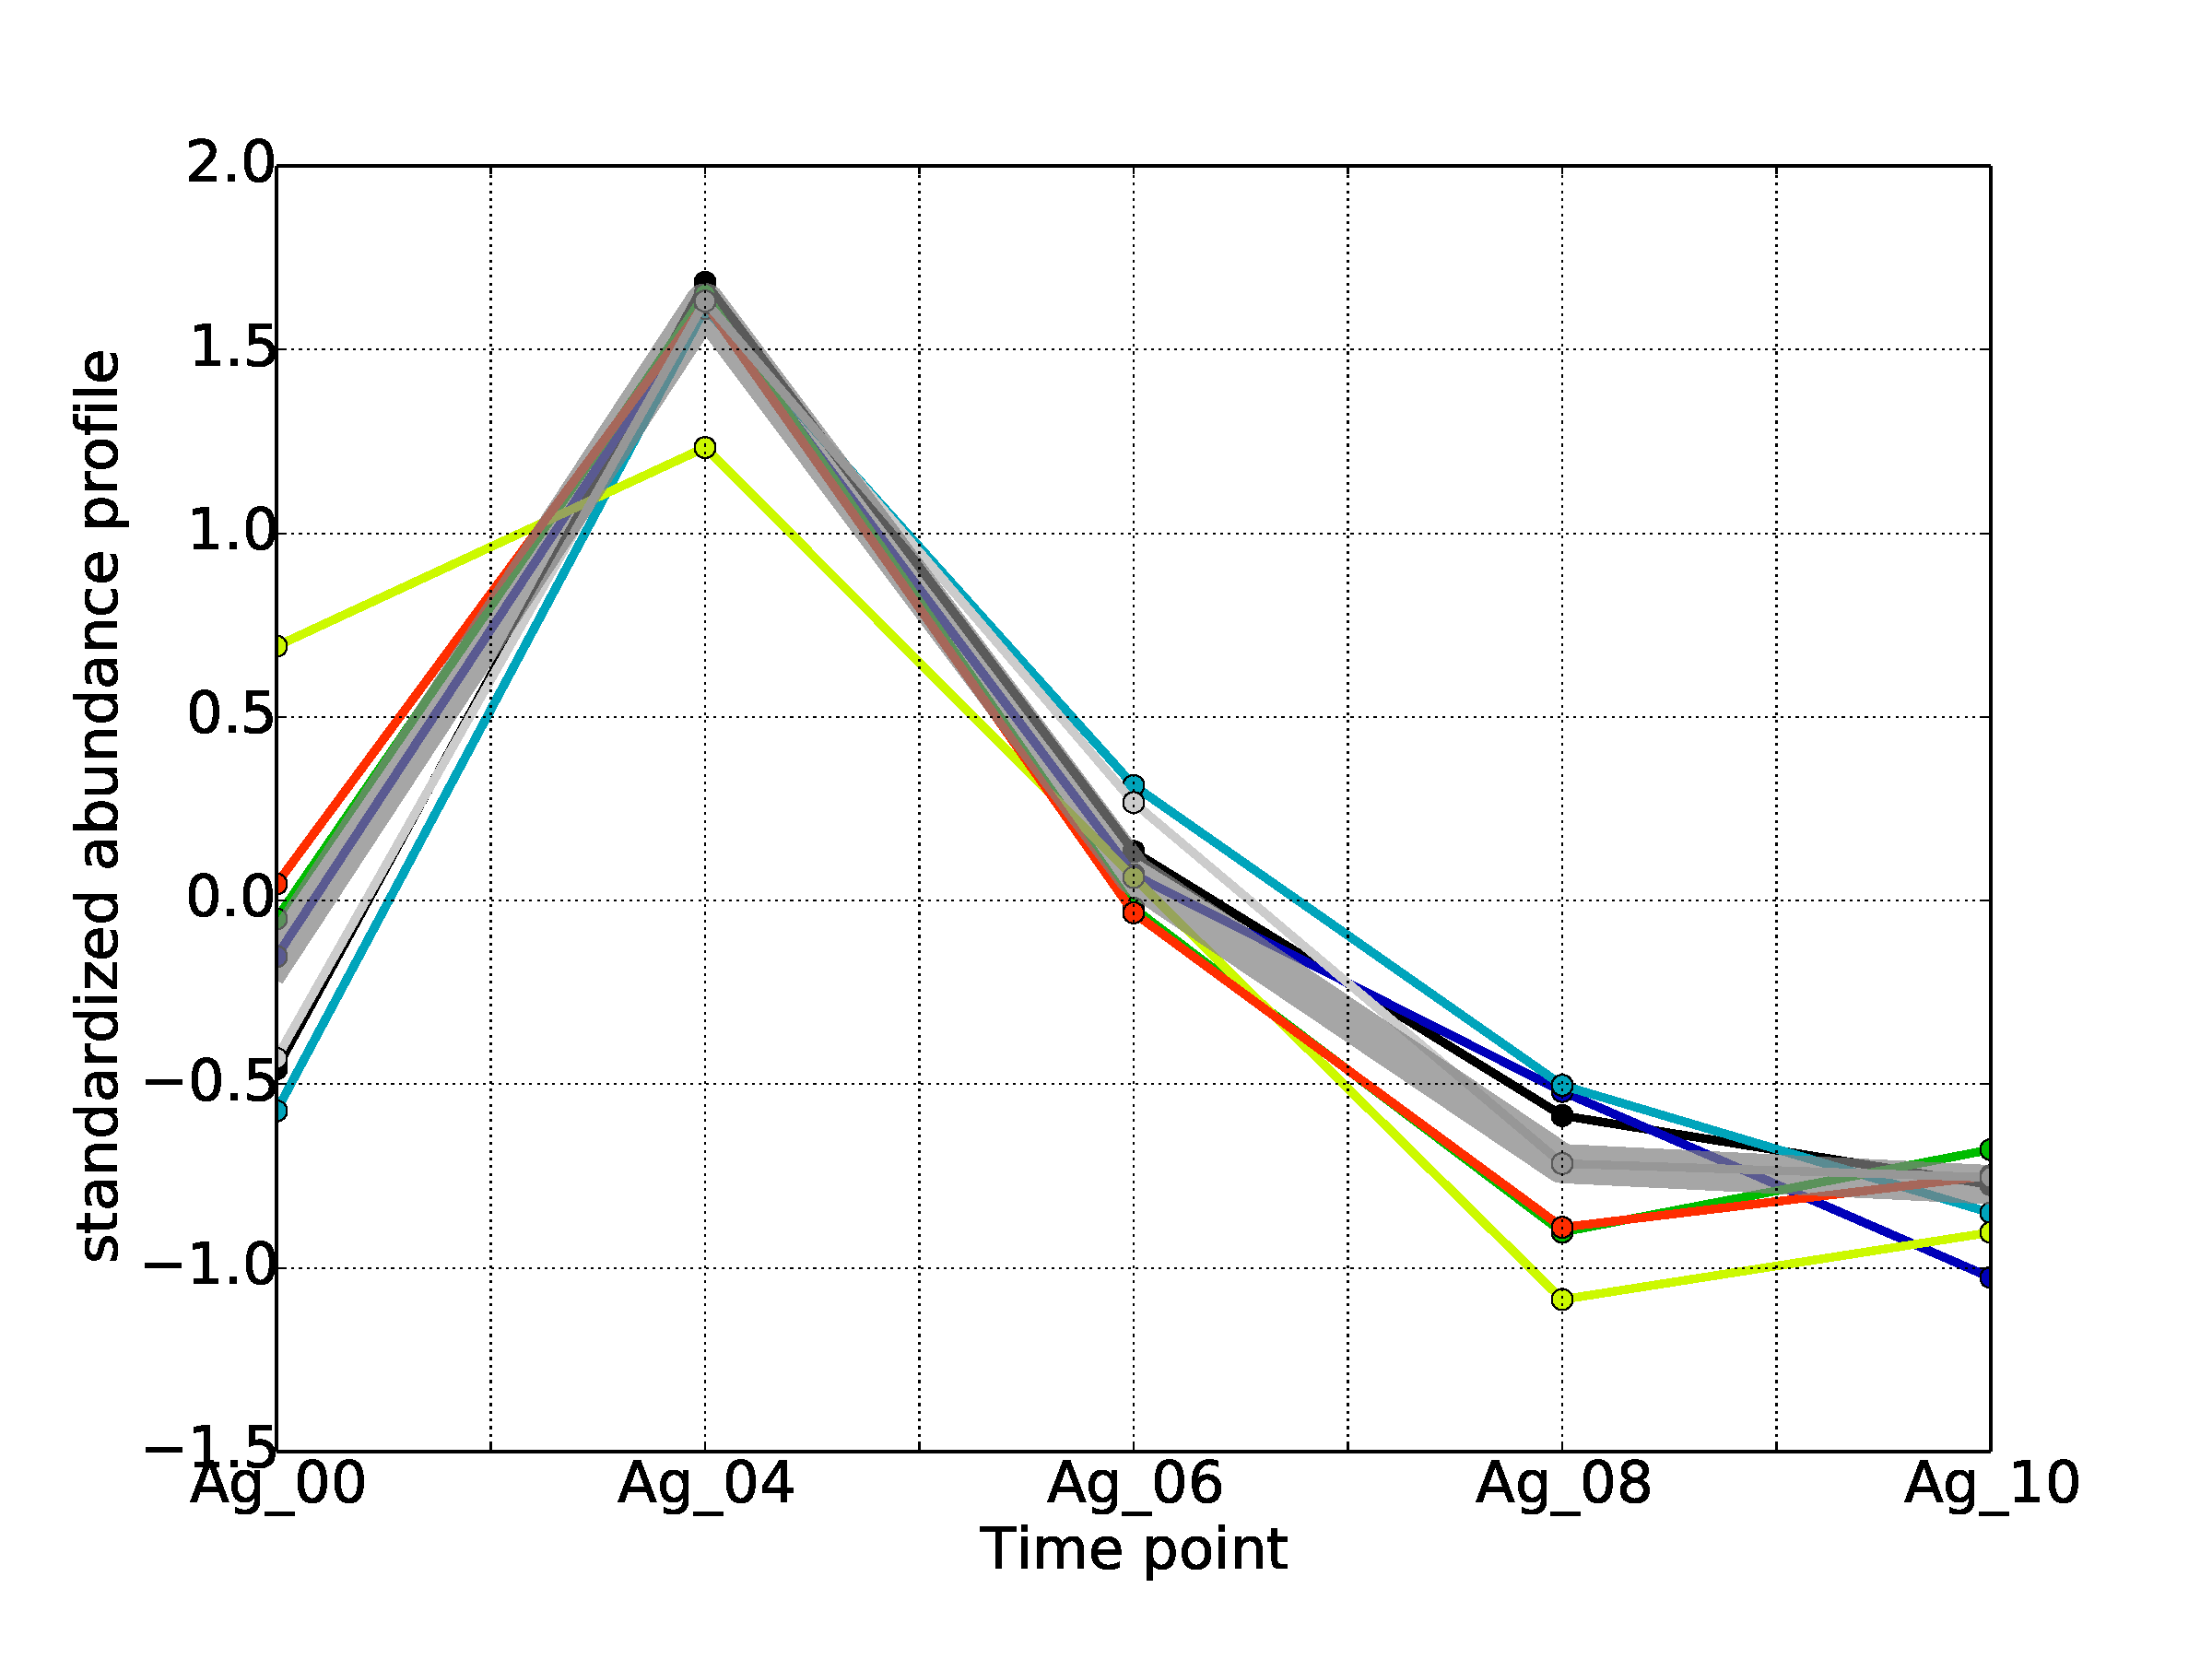
\includegraphics[width=.5\linewidth]{figures/figs/ecr_and_insects_ptci_20130918_orthodb7/upAt4_gene_profiles_from_cummerbund/Ag_upAt4_cls22_Ag_target_FPKMs_vb_orthos.pdf}}
%
\subcaptionbox{\label{fig:cluster22-Cq}}
{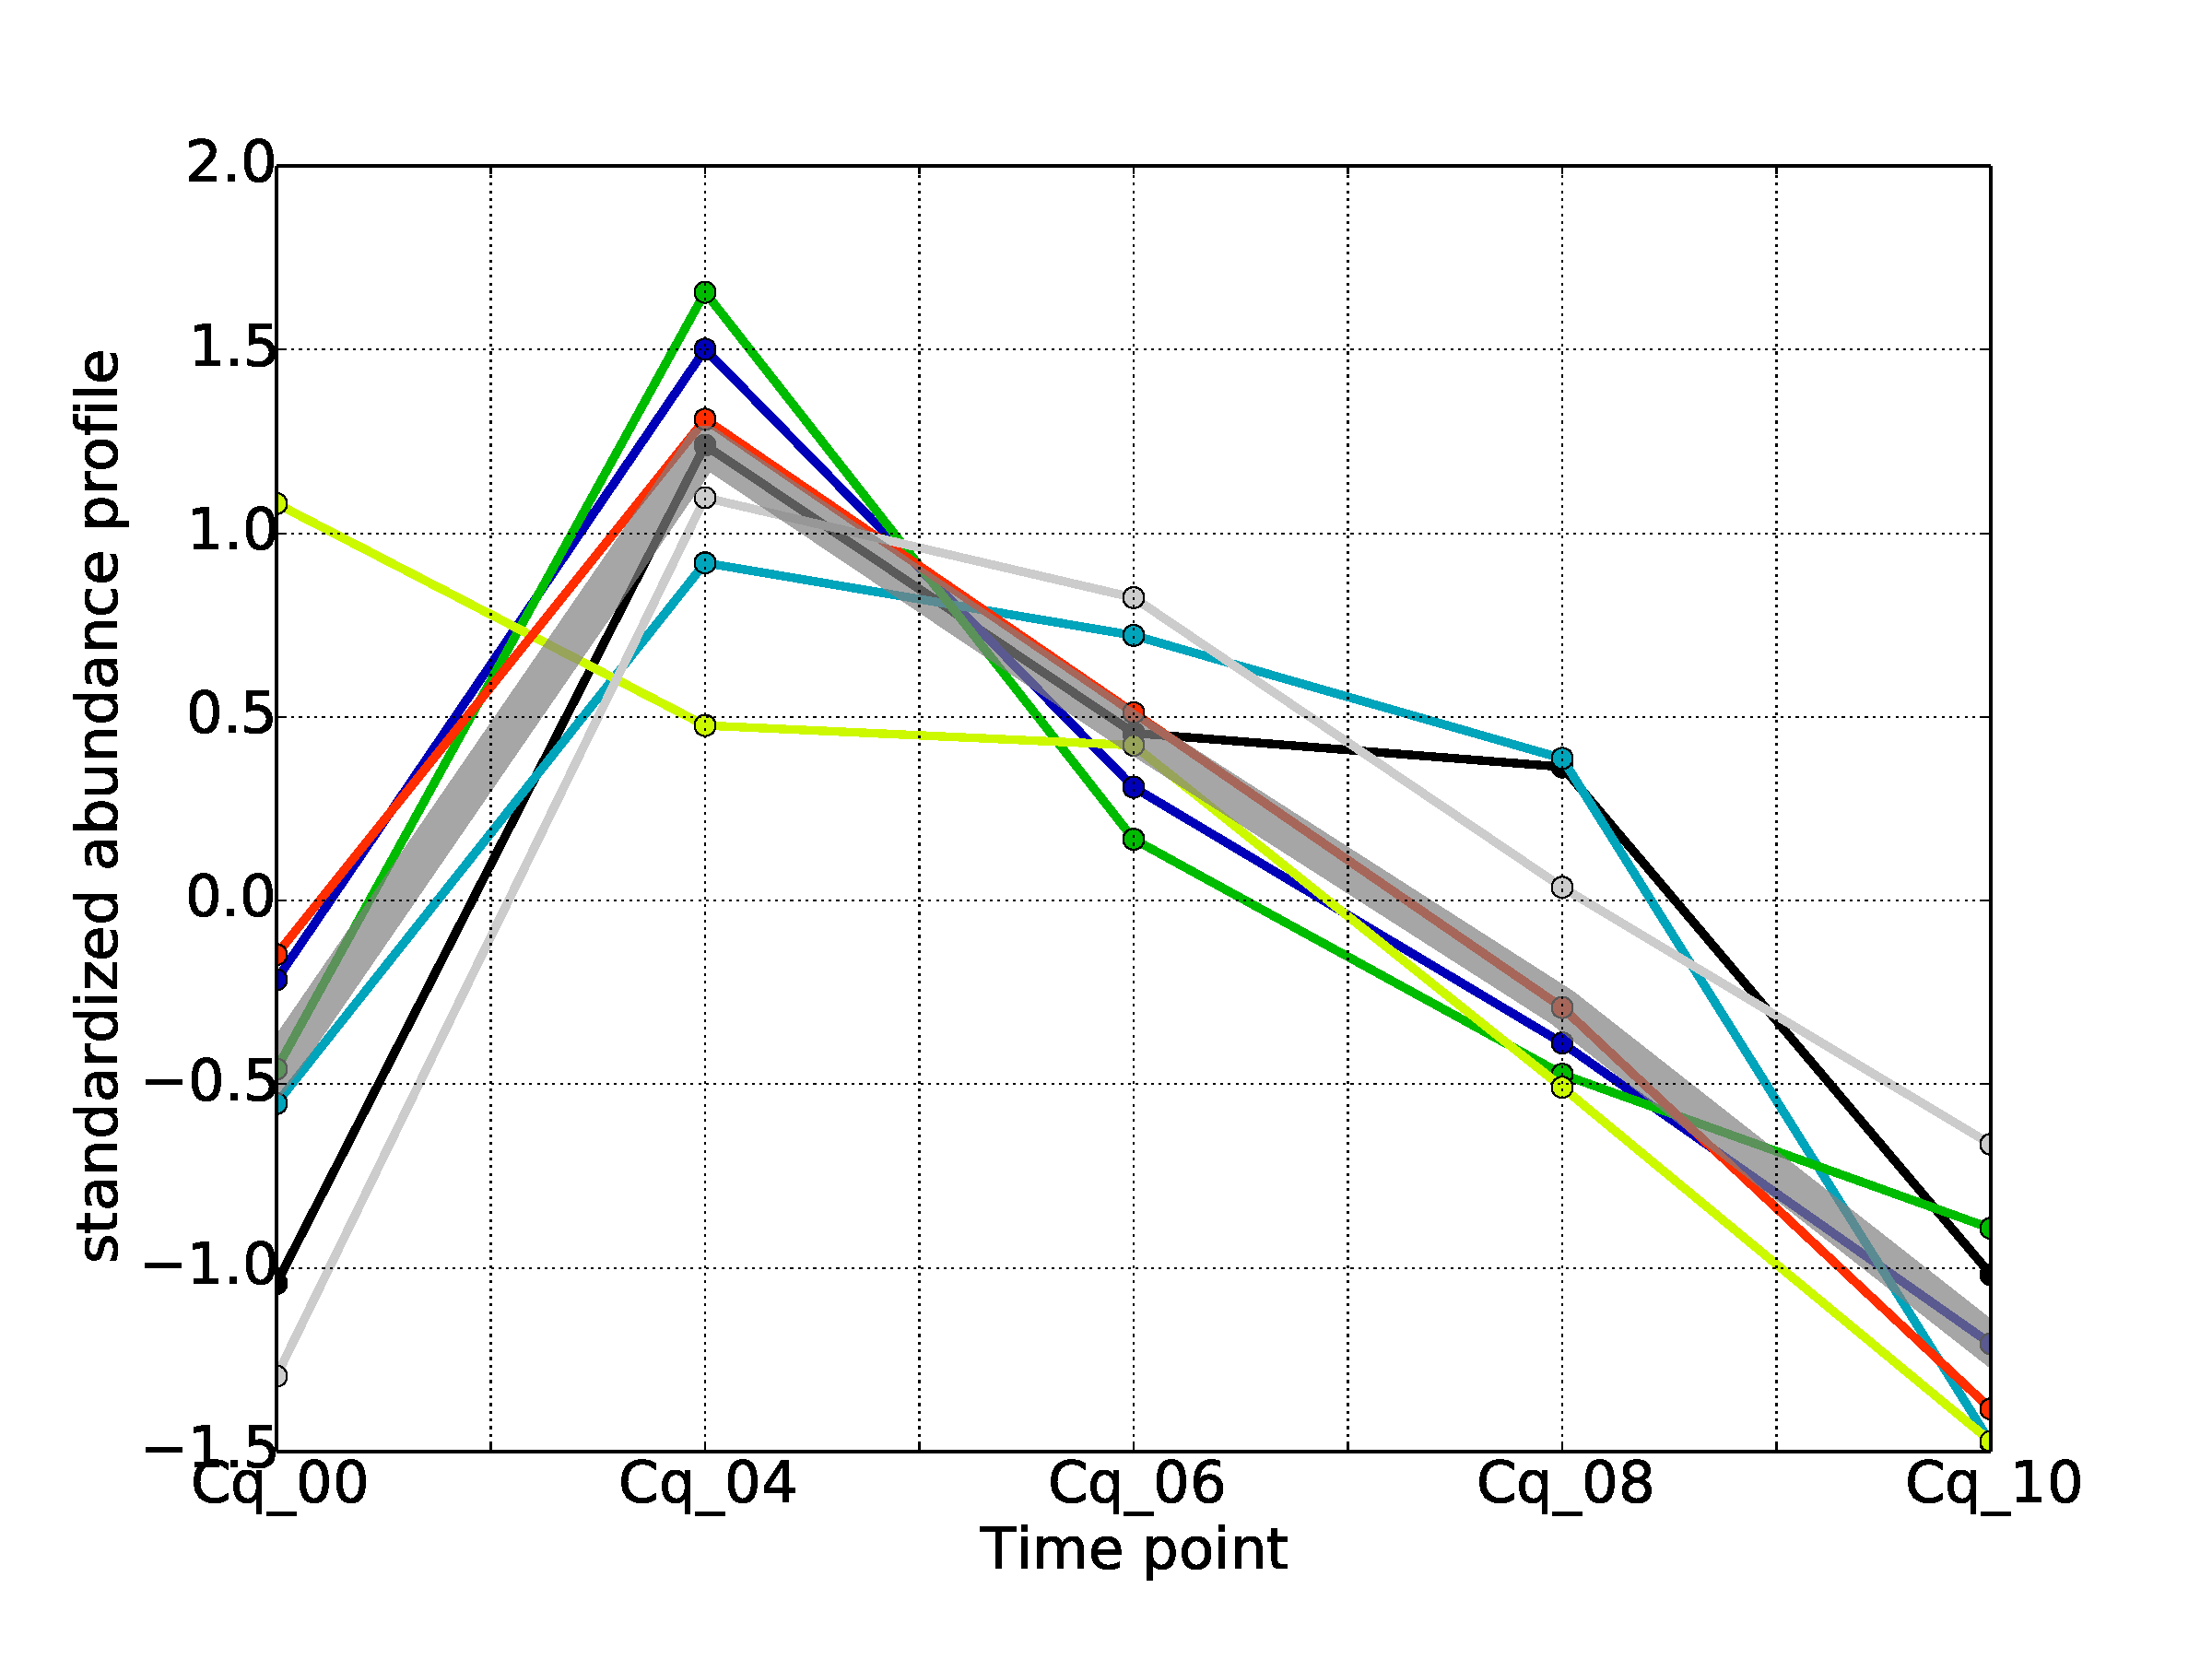
\includegraphics[width=.5\linewidth]{figures/figs/ecr_and_insects_ptci_20130918_orthodb7/upAt4_gene_profiles_from_cummerbund/Cq_upAt4_cls22_Ag_target_FPKMs_vb_orthos.pdf}}
% 
\caption[Orthologs of cluster 22]{\sf \textbf{Orthologs of cluster 22 (up at 4h):}\\
The same color scheme is used for each species which means that orthologs are given the same color in all three panels.
The thick, transparent gray line represents the median \gls{mAP} for the panel.
\textbf{(A)} \Aa.
\textbf{(B)} \Ag.
\textbf{(C)} \Cq.
}\label{fig:cluster22}
\end{figure}

\subsection{K-means clustering}

K-means clustering ($k=23$) was applied to the 310 genes from \Ag\ to attempt to partition the 3-way 1:1 ortholog sets based on \gls{mAP} similarity.
%
\Ag\ was selected because it shares approximately equidistant evolutionary divergence to both other species.
%
Four of the resulting clusters were chosen for further characterization (Figure \ref{fig:23-clusters}: \textit{Cluster IDs 4, 6, 16, and 22}) because they have expression patterns that may be regulated by a noted pulse of \gls{20E} that occurs around 4h \gls{PBM}\footnote{See Section \ref{chap:3-sec:clustering-of-filtered-ortholog-sets} for more information.}.
%




% cls4
% Booktabs require to add \usepackage{booktabs} to your document preamble
\begin{table}[hp]
\begin{center} \sf
\begin{tabular}{p{.7\textwidth}r}
\toprule
\textbf{Name}                                                 & \textbf{Total Score (mean)} \\ \midrule
SRP-dependent cotranslational protein targeting to membrane   & 13254.87                    \\ % secretion / nutrient pathway
Golgi organization                                            & 7289.78                     \\ % secretion / nutrient pathway
glutamine biosynthetic process                                & 7056.26                     \\
bone development                                              & 6844.92                     \\ % #EXPLAIN #LOOKUP << LOOK HERE: http://pfam.sanger.ac.uk/family/PF09742 --> Functionally this protein might be involved in vesicle secretion or be an inter-cellular signalling protein or be a novel insulin receptor.[PMID 14504222] >>
ER to Golgi vesicle-mediated transport                        & 5914.05                     \\
heme biosynthetic process                                     & 5069.12                     \\ % bloodmeal
regulation of translational initiation                        & 4594.46                     \\ % translation/ TOR?
formation of translation preinitiation complex                & 4524.89                     \\ % translation/ TOR?
translational initiation                                      & 4288.82                     \\
translation                                                   & 3777.61                     \\
% positive regulation of GTPase activity                        & 3543.72                     \\
proteasome assembly                                           & 3326.44                     \\ % upregulated translation
porphyrin-containing compound biosynthetic process            & 3077.12                     \\ % #EXPLAIN #LOOKUP {{ferrochetalase}}
proton transport                                              & 2772.26                     \\ % digestion? endocytosis?
% ATP catabolic process                                         & 2642.02                     \\ % consumption of ATP / energy for proton transport?
proteolysis                                                   & 2453.58                     \\ % digestion
regulation of autophagy                                       & 2294.64                     \\ % change from starvation to nutrient excess
retrograde vesicle-mediated transport, Golgi to ER            & 2202.55                     \\
L-lysine catabolic process to acetyl-CoA via saccharopine     & 2148.61                     \\
vesicle fusion with Golgi apparatus                           & 2141.47                     \\
proteolysis involved in cellular protein catabolic process    & 1972.16                     \\
ubiquitin-dependent protein catabolic process                 & 1963.42                     \\
nitrogen compound metabolic process                           & 1885.16                     \\ % #EXPLAIN
ATP hydrolysis coupled proton transport                       & 1860.32                     \\ 
cell-cell adhesion                                            & 1774.89                     \\ % Midgut repair?
small GTPase mediated signal transduction                     & 1693.93                     \\
% response to drug                                              & 1507.48                     \\
% Golgi vesicle transport                                       & 1410.43                     \\
% intracellular protein transport                               & 1382.58                     \\
oligopeptide transport                                        & 1243.85                     \\
% cellular membrane fusion                                      & 1216.84                     \\
protein ubiquitination                                        & 1073.12                     \\
transmembrane transport                                       & 1025.68                     \\
vesicle-mediated transport                                    & 930.96                      \\
% protein transport                                             & 905.51                      \\
% mitotic prophase                                              & 897.77                      \\
% peptide transport                                             & 721.42                      \\
% transport                                                     & 657.84                      \\
% oocyte growth                                                 & 543.51                      \\ % endoplasmic reticulum organization and vesical trafficing (this gene known important in nurse cell folicle relationship) {{Protein jagunal}}
ion transport                                                 & 480.36                      \\
glycine biosynthetic process, by transamination of glyoxylate & 464.76                      \\
autophagy                                                     & 447.12                      \\
L-lysine catabolic process                                    & 417.84                      \\
lysine catabolic process                                      & 414.33                      \\
% oogenesis                                                     & 406.52                      \\
L-cysteine catabolic process                                  & 378.10                      \\
exocytosis                                                    & 294.15                      \\ % digestive secretion ? {{Protein jagunal}} endoplasmic reticulum organization and vesical trafficing
% cell adhesion                                                 & 286.17                      \\
cell differentiation                                          & 279.02                      \\ % midgut repair ?
detoxification of cadmium ion                                 & 262.31                      \\
% multicellular organismal development                          & 253.99                      \\
small molecule metabolic process                              & 253.25                      \\
metabolic process                                             & 235.09                      \\
cellular nitrogen compound metabolic process                  & 234.76                      \\
lysine biosynthetic process                                   & 207.74                      \\
cellular amino acid biosynthetic process                      & 200.81                      \\ \bottomrule                                                           
\end{tabular}
\end{center}

\caption[Cluster 4 top process GO terms]{\sf \textbf{Cluster 4 top process GO terms}}
\label{tab:cls4-process}
\end{table}
Table \ref{tab:cls4-process}
% Booktabs require to add \usepackage{booktabs} to your document preamble
\begin{table}[hp]
\begin{center} \sf
\begin{tabular}{p{.7\textwidth}r}
\toprule
\textbf{Name}                                                                                  & \textbf{Total Score (mean)} \\ \midrule
translation initiation factor activity                                                         & 18796.17                    \\ % translation/ TOR?
protein transporter activity                                                                   & 13663.10                    \\
signal recognition particle binding                                                            & 9157.88                     \\
endoplasmic reticulum signal peptide binding                                                   & 7943.20                     \\ % secretion 
Rab GDP-dissociation inhibitor activity                                                        & 7361.38                     \\
hydrolase activity, acting on acid anhydrides, catalyzing transmembrane movement of substances & 6647.91                     \\
hydrogen ion transmembrane transporter activity                                                & 6278.87                     \\
ferrochelatase activity                                                                        & 4990.12                     \\
GTP binding                                                                                    & 4006.06                     \\
%enzyme binding                                                                                 & 3697.54                     \\
saccharopine dehydrogenase (NAD+, L-glutamate-forming) activity                                & 3453.61                     \\
zinc ion binding                                                                               & 3215.15                     \\
glutamate-ammonia ligase activity                                                              & 2901.02                     \\
RNA binding                                                                                    & 2799.62                     \\
ATPase activity, coupled to transmembrane movement of substances                               & 2678.79                     \\
pyridoxal phosphate binding                                                                    & 2586.25                     \\
transporter activity                                                                           & 2044.78                     \\
saccharopine dehydrogenase (NADP+, L-lysine-forming) activity                                  & 1890.88                     \\
threonine-type endopeptidase activity                                                          & 1842.63                     \\
GTPase activator activity                                                                      & 1780.38                     \\
transaminase activity                                                                          & 1686.97                     \\
aminopeptidase activity                                                                        & 1592.00                     \\
endopeptidase activity                                                                         & 1546.38                     \\
nucleoside-triphosphatase activity                                                             & 1372.39                     \\
ATPase activity                                                                                & 1369.37                     \\
hydrolase activity                                                                             & 1352.33                     \\
lyase activity                                                                                 & 1299.81                     \\
ubiquitin-protein ligase activity                                                              & 1261.81                     \\
oxidoreductase activity                                                                        & 1237.14                     \\
nucleotide binding                                                                             & 1166.69                     \\
GTPase activity                                                                                & 1110.62                     \\
protein binding                                                                                & 1013.21                     \\
oligopeptide transporter activity                                                              & 927.01                      \\
symporter activity                                                                             & 915.24                      \\
ligase activity                                                                                & 870.70                      \\
metallopeptidase activity                                                                      & 809.99                      \\
metal ion binding                                                                              & 794.06                      \\
peptidase activity                                                                             & 792.59                      \\
proton-transporting ATPase activity, rotational mechanism                                      & 702.75                      \\
% ATP binding                                                                                    & 662.73                      \\
% catalytic activity                                                                             & 438.09                      \\
transferase activity                                                                           & 319.82                      \\
dipeptide transporter activity                                                                 & 217.58                      \\ \bottomrule
\end{tabular}
\end{center}

\caption[Cluster 4 (up after 4h) mean function GO terms]{\sf \textbf{Cluster 4 (up after 4h) mean function GO terms}}
\label{tab:cls4-function}
\end{table}
Table \ref{tab:cls4-function}
% % Booktabs require to add \usepackage{booktabs} to your document preamble
\begin{table}[h]
\begin{center} \sf
\begin{tabular}{@{}lr@{}}
\toprule
\textbf{Name}                                                & \textbf{Total Score (mean)} \\ \midrule
signal recognition particle, endoplasmic reticulum targeting & 7479.07                     \\
vacuolar proton-transporting V-type ATPase complex           & 4776.11                     \\
proton-transporting V-type ATPase, V0 domain                 & 3723.39                     \\
eukaryotic 48S preinitiation complex                         & 3378.14                     \\ % translation/ TOR?
eukaryotic 43S preinitiation complex                         & 3377.91                     \\ % translation/ TOR?
clathrin adaptor complex                                     & 2970.27                     \\ % digestive 
proteasome core complex                                      & 2849.33                     \\ % translation upregulation
ribonucleoprotein complex                                    & 2232.37                     \\
peroxisome                                                   & 2058.24                     \\
proteasome complex                                           & 2009.89                     \\
cytoplasm                                                    & 1225.49                     \\
mitochondrion                                                & 1210.38                     \\
COPII vesicle coat                                           & 1194.53                     \\
Golgi membrane                                               & 1054.43                     \\
proteasome accessory complex                                 & 1051.54                     \\
COPI vesicle coat                                            & 946.99                      \\
Golgi apparatus                                              & 896.79                      \\
integral to membrane                                         & 888.57                      \\
endoplasmic reticulum membrane                               & 768.50                      \\
nucleolus                                                    & 759.14                      \\
cytoplasmic vesicle                                          & 754.11                      \\
proteasome core complex, alpha-subunit complex               & 749.91                      \\
intracellular                                                & 685.04                      \\
membrane                                                     & 617.44                      \\
nucleus                                                      & 575.67                      \\
ER membrane protein complex                                  & 549.36                      \\
mitochondrial inner membrane                                 & 493.51                      \\
COPI-coated vesicle membrane                                 & 480.43                      \\
peroxisomal matrix                                           & 455.49                      \\
ER to Golgi transport vesicle membrane                       & 420.45                      \\
mitochondrial outer membrane                                 & 381.02                      \\
endoplasmic reticulum                                        & 373.40                      \\
autophagic vacuole membrane                                  & 370.40                      \\
vacuolar membrane                                            & 360.81                      \\
vacuole                                                      & 313.06                      \\
intracellular membrane-bounded organelle                     & 303.53                      \\
phagocytic vesicle                                           & 273.00                      \\
recycling endosome                                           & 236.71                      \\
synaptic vesicle membrane                                    & 219.28                      \\
protein complex                                              & 203.31                      \\ \bottomrule
\end{tabular}
\end{center}

\caption[Cluster 4 top cellular GO terms]{\sf \textbf{Cluster 4 top cellular GO terms}}
\label{tab:cls4-cellular}
\end{table}
% Table \ref{tab:cls4-cellular}

% cls6
% Booktabs require to add \usepackage{booktabs} to your document preamble
\begin{table}[hp]
\begin{center} \sf
\begin{tabular}{p{.7\textwidth}r}
\toprule
\textbf{Name}                                                           & \textbf{Total Score (mean)} \\ \midrule
Mo-molybdopterin cofactor biosynthetic process                          & 7762.64                     \\ % #LOOKUP
GTP catabolic process                                                   & 5712.72                     \\
translational elongation                                                & 3558.74                     \\
heme biosynthetic process                                               & 2615.06                     \\ % heme managment
glutamate biosynthetic process                                          & 2418.17                     \\
protein export from nucleus                                             & 2157.87                     \\
translation                                                             & 1962.19                     \\ % translation
cellular amino acid biosynthetic process                                & 1737.45                     \\
sex differentiation                                                     & 1549.60                     \\ % #EXPLAIN this is DBX
nuclear-transcribed mRNA catabolic process, nonsense-mediated decay     & 1190.98                     \\ % #LOOKUP
biosynthetic process                                                    & 1116.03                     \\
regulation of cyclin-dependent protein serine/threonine kinase activity & 950.21                      \\ % #LOOKUP CyclinT
cell adhesion                                                           & 938.98                      \\
intracellular protein transport                                         & 853.03                      \\
glutamine metabolic process                                             & 826.49                      \\
steroid hormone mediated signaling pathway                              & 779.04                      \\ % #LOOKUP (AGAP005661:AAEL002062:CPIJ014945 Ftz transcription factor)
protoporphyrinogen IX biosynthetic process                              & 769.19                      \\ % #LOOKUP Heme Biosynth
regulation of transcription, DNA-dependent                              & 760.48                      \\ 
nitrogen compound metabolic process                                     & 726.25                      \\
rRNA processing                                                         & 660.29                      \\
SRP-dependent cotranslational protein targeting to membrane             & 653.41                      \\
tetrapyrrole biosynthetic process                                       & 607.64                      \\
ribosome biogenesis                                                     & 571.22                      \\
transport                                                               & 489.46                      \\
transcription, DNA-dependent                                            & 454.23                      \\
protein transport                                                       & 449.05                      \\
cell-matrix adhesion                                                    & 339.59                      \\
Wnt receptor signaling pathway                                          & 330.08                      \\
nucleosome disassembly                                                  & 285.68                      \\ % 1:1 ortho of Dmel: Brahma associated protein 170kD [Bap170]
actin filament bundle assembly                                          & 281.75                      \\
metabolic process                                                       & 270.58                      \\
protein phosphorylation                                                 & 263.56                      \\
enzyme active site formation via L-cysteine persulfide                  & 228.92                      \\
synapse assembly                                                        & 222.33                      \\
regulation of protein export from nucleus                               & 214.34                      \\
neurogenesis                                                            & 212.84                      \\ \bottomrule
\end{tabular}
\end{center}

\caption[Cluster 6 top process GO terms]{\sf \textbf{Cluster 6 top process GO terms}}
\label{tab:cls6-process}
\end{table}
Table \ref{tab:cls6-process}
% Booktabs require to add \usepackage{booktabs} to your document preamble
\begin{table}[h]
\begin{center} \sf
\begin{tabular}{p{.7\textwidth}r}
\toprule
\textbf{Name}                                                 & \textbf{Total Score (mean)} \\ \midrule
protein transporter activity                                  & 9225.37                     \\
translation elongation factor activity                        & 4478.17                     \\ % #EXPLAIN
GTPase activity                                               & 4364.13                     \\
GTP binding                                                   & 3823.91                     \\
phospholipid binding                                          & 3341.66                     \\
pyridoxal phosphate binding                                   & 2871.76                     \\
steroid hormone receptor activity                             & 2322.77                     \\ % which gene(s) is this?
protein kinase binding                                        & 2059.25                     \\
sequence-specific DNA binding                                 & 1999.76                     \\ % transcription factor repression?
protein N-terminus binding                                    & 1781.39                     \\
protein complex binding                                       & 1446.01                     \\
transferase activity, transferring acyl groups                & 1047.27                     \\
integrin binding                                              & 1003.53                     \\
protein domain specific binding                               & 995.27                      \\
DNA binding                                                   & 910.28                      \\ % transcription factor repression?
ATP-dependent helicase activity                               & 877.71                      \\
carboxylesterase activity                                     & 828.49                      \\
sequence-specific DNA binding transcription factor activity   & 796.99                      \\ % transcription factor repression?
nucleotide binding                                            & 772.48                      \\ % transcription factor repression?
hydrolase activity                                            & 766.78                      \\
helicase activity                                             & 737.95                      \\ % #EXPLAIN
ATP binding                                                   & 700.66                      \\
glutamate synthase activity                                   & 578.54                      \\
zinc ion binding                                              & 578.26                      \\ % transcription factor repression?
protein binding                                               & 569.78                      \\
GTPase regulator activity                                     & 568.11                      \\
transferase activity                                          & 536.16                      \\
oxidoreductase activity                                       & 512.70                      \\
protein dimerization activity                                 & 503.19                      \\
nucleic acid binding                                          & 500.17                      \\
oxidoreductase activity, acting on the CH-NH2 group of donors & 461.69                      \\
metal ion binding                                             & 453.98                      \\
kinesin binding                                               & 450.65                      \\
JUN kinase binding                                            & 392.02                      \\ % #EXPLAIN
phosphatidylinositol-3,4,5-trisphosphate binding              & 387.10                      \\
lipid binding                                                 & 367.29                      \\
RNA binding                                                   & 316.90                      \\
protein homodimerization activity                             & 309.12                      \\ % transcription factor repression?
catalytic activity                                            & 263.32                      \\
glutamate synthase (ferredoxin) activity                      & 254.70                      \\ % #EXPLAIN
transporter activity                                          & 233.90                      \\ \bottomrule
\end{tabular}
\end{center}

\caption[Cluster 6 top function GO terms]{\sf \textbf{Cluster 6 top function GO terms}}
\label{tab:cls6-function}
\end{table}
Table \ref{tab:cls6-function}
% % Booktabs require to add \usepackage{booktabs} to your document preamble
\begin{table}[h]
\begin{center} \sf
\begin{tabular}{@{}lr@{}}
\toprule
\textbf{Name}                                      & \textbf{Total Score (mean)} \\ \midrule
cytosol                                            & 11598.25                    \\
mitochondrial matrix                               & 5271.13                     \\
nucleus                                            & 3895.71                     \\
plastid                                            & 2414.67                     \\
chloroplast stroma                                 & 2058.69                     \\
chloroplast                                        & 1874.07                     \\
nuclear pore                                       & 1453.16                     \\
positive transcription elongation factor complex b & 1281.93                     \\
mitochondrion                                      & 1208.52                     \\
cytoplasm                                          & 1095.77                     \\
intracellular                                      & 970.52                      \\
signal recognition particle                        & 809.92                      \\
focal adhesion                                     & 735.87                      \\
ribonucleoprotein complex                          & 669.27                      \\
cell junction                                      & 666.19                      \\
spliceosomal complex                               & 587.46                      \\
synapse                                            & 481.27                      \\
cell projection                                    & 442.30                      \\
dynein complex                                     & 343.74                      \\
plasma membrane                                    & 317.82                      \\
lamellipodium membrane                             & 302.49                      \\
filamentous actin                                  & 260.41                      \\
nuclear body                                       & 250.79                      \\
lamellipodium                                      & 227.79                      \\
actin filament                                     & 226.01                      \\
membrane                                           & 216.49                      \\
mitochondrial inner membrane                       & 216.01                      \\ \bottomrule
\end{tabular}
\end{center}

\caption[Cluster 6 top cellular GO terms]{\sf \textbf{Cluster 6 top cellular GO terms}}
\label{tab:cls6-cellular}
\end{table}
% Table \ref{tab:cls6-cellular}

% cls16
% Booktabs require to add \usepackage{booktabs} to your document preamble
\begin{table}[h]
\begin{center} \sf
\begin{tabular}{p{.7\textwidth}r}
\toprule
\textbf{Name}                                 & \textbf{Total Score (mean)} \\ \midrule
one-carbon metabolic process                  & 8498.68                     \\
carbohydrate metabolic process                & 4077.43                     \\
translation                                   & 3505.77                     \\
regulation of Rho protein signal transduction & 1336.90                     \\
homophilic cell adhesion                      & 1316.75                     \\
cell adhesion                                 & 851.76                      \\
autophagy                                     & 686.01                      \\
apoptotic process                             & 670.22                      \\
regulation of myelination                     & 618.20                      \\
protein phosphorylation                       & 542.93                      \\
phosphorylation                               & 395.02                      \\
metabolic process                             & 286.58                      \\
protein transport                             & 262.15                      \\
protein ubiquitination                        & 242.49                      \\
intracellular signal transduction             & 212.22                      \\ \bottomrule
\end{tabular}
\end{center}

\caption[Cluster 16 top process GO terms]{\sf \textbf{Cluster 16 top process GO terms}}
\label{tab:cls16-process}
\end{table}
Table \ref{tab:cls16-process}
% Booktabs require to add \usepackage{booktabs} to your document preamble
\begin{table}[h]
\begin{center} \sf
\begin{tabular}{p{.7\textwidth}r}
\toprule
\textbf{Name}                                                    & \textbf{Total Score (mean)} \\ \midrule
carbonate dehydratase activity                                   & 4264.07                     \\
cysteine-type peptidase activity                                 & 2253.39                     \\
carbon-nitrogen ligase activity, with glutamine as amido-N-donor & 1652.90                     \\
Rho guanyl-nucleotide exchange factor activity                   & 1446.25                     \\
zinc ion binding                                                 & 1412.73                     \\
guanyl-nucleotide exchange factor activity                       & 1208.72                     \\
nucleic acid binding                                             & 810.14                      \\
peptidase activity                                               & 715.27                      \\
beta-tubulin binding                                             & 707.48                      \\
hydrolase activity, acting on glycosyl bonds                     & 652.43                      \\
glutaminyl-tRNA synthase (glutamine-hydrolyzing) activity        & 550.56                      \\
protein binding                                                  & 433.44                      \\
protein serine/threonine kinase activity                         & 413.31                      \\
metal ion binding                                                & 408.70                      \\
microtubule binding                                              & 403.62                      \\
ATP binding                                                      & 395.77                      \\
transferase activity                                             & 387.71                      \\
maltose alpha-glucosidase activity                               & 378.58                      \\
hydrolase activity                                               & 366.71                      \\
catalytic activity                                               & 331.87                      \\
ligase activity                                                  & 310.07                      \\
alpha-glucosidase activity                                       & 285.38                      \\
nucleotide binding                                               & 239.99                      \\
lyase activity                                                   & 212.94                      \\
oxidoreductase activity                                          & 206.49                      \\
protein kinase activity                                          & 200.95                      \\ \bottomrule                   
\end{tabular}
\end{center}

\caption[Cluster 16 top function GO terms]{\sf \textbf{Cluster 16 top function GO terms}}
\label{tab:cls16-function}
\end{table}
Table \ref{tab:cls16-function}
% % Booktabs require to add \usepackage{booktabs} to your document preamble
\begin{table}[h]
\begin{center} \sf
\begin{tabular}{@{}lr@{}}
\toprule
\textbf{Name}                      & \textbf{Total Score (mean)} \\ \midrule
lysosome                           & 3960.21                     \\
nucleus                            & 1277.31                     \\
integral to membrane               & 943.86                      \\
nucleolus                          & 781.11                      \\
membrane                           & 615.70                      \\
SCF ubiquitin ligase complex       & 572.11                      \\
Cul4-RING ubiquitin ligase complex & 563.83                      \\
plasma membrane                    & 527.87                      \\
cytoplasm                          & 488.72                      \\
intracellular                      & 484.82                      \\
cytoskeleton                       & 305.53                      \\ \bottomrule
\end{tabular}
\end{center}

\caption[Cluster 16 top cellular GO terms]{\sf \textbf{Cluster 16 top cellular GO terms}}
\label{tab:cls16-cellular}
\end{table}
% Table \ref{tab:cls16-cellular}

% cls22
% Booktabs require to add \usepackage{booktabs} to your document preamble
\begin{table}[hp]
\begin{center} \sf
\begin{tabular}{p{.7\textwidth}r}
\toprule
\textbf{Name}                                  & \textbf{Total Score (mean)} \\ \midrule
lysyl-tRNA aminoacylation                      & 5305.29                     \\
regulation of translational initiation         & 5198.13                     \\
protein folding                                & 5145.48                     \\
translation                                    & 3885.25                     \\
tRNA aminoacylation for protein translation    & 3277.15                     \\
translational initiation                       & 3268.53                     \\
cellular protein metabolic process             & 2591.65                     \\
regulation of transcription, DNA-dependent     & 2500.50                     \\
transmembrane transport                        & 2120.54                     \\
formation of translation preinitiation complex & 1607.78                     \\
transcription, DNA-dependent                   & 1314.06                     \\
signal transduction                            & 853.12                      \\
regulation of insulin secretion                & 709.97                      \\
negative regulation of BMP signaling pathway   & 526.20                      \\
regulation of cell cycle                       & 470.82                      \\
melanocyte differentiation                     & 316.77                      \\
endocrine pancreas development                 & 296.05                      \\
transport                                      & 288.59                      \\
developmental pigmentation                     & 287.51                      \\
pigmentation                                   & 273.58                      \\
tRNA processing                                & 223.64                      \\
multicellular organismal development           & 203.63                      \\ \bottomrule
\end{tabular}
\end{center}

\caption[Cluster 22 top process GO terms]{\sf \textbf{Cluster 22 top process GO terms}}
\label{tab:cls22-process}
\end{table}
Table \ref{tab:cls22-process}
% Booktabs require to add \usepackage{booktabs} to your document preamble
\begin{table}[hp]
\begin{center} \sf
\begin{tabular}{p{.7\textwidth}r}
\toprule
\textbf{Name}                               & \textbf{Total Score (mean)} \\ \midrule
translation initiation factor activity      & 20221.31                    \\
unfolded protein binding                    & 7160.14                     \\
DNA binding                                 & 4535.66                     \\
arsenite transmembrane transporter activity & 1600.53                     \\
lysine-tRNA ligase activity                 & 1557.61                     \\
cytoskeletal adaptor activity               & 1456.65                     \\
ATP binding                                 & 1146.99                     \\
aminoacyl-tRNA ligase activity              & 682.47                      \\
nucleotide binding                          & 669.32                      \\
ligase activity                             & 526.89                      \\
transporter activity                        & 400.96                      \\
zinc ion binding                            & 257.13                      \\ \bottomrule                     
\end{tabular}
\end{center}

\caption[Cluster 22 (up at 4h) mean function GO terms]{\sf \textbf{Cluster 22 (up at 4h) mean function GO terms}}
\label{tab:cls22-function}
\end{table}
Table \ref{tab:cls22-function}
% % Booktabs require to add \usepackage{booktabs} to your document preamble
\begin{table}[h]
\begin{center} \sf
\begin{tabular}{@{}lr@{}}
\toprule
\textbf{Name}                                      & \textbf{Total Score (mean)} \\ \midrule
eukaryotic translation initiation factor 3 complex & 9146.56                     \\
integral to nuclear inner membrane                 & 6268.74                     \\
chaperonin-containing T-complex                    & 4904.34                     \\
cytoplasm                                          & 3337.48                     \\
eukaryotic 43S preinitiation complex               & 3196.30                     \\
eukaryotic 48S preinitiation complex               & 3129.90                     \\
nucleus                                            & 1534.04                     \\
lysosomal membrane                                 & 1133.53                     \\
integral to membrane                               & 996.11                      \\
cytosol                                            & 520.36                      \\
nuclear envelope                                   & 469.02                      \\
membrane                                           & 281.10                      \\
nuclear inner membrane                             & 219.28                      \\
nucleolus                                          & 203.40                      \\ \bottomrule
\end{tabular}
\end{center}

\caption[Cluster 22 top cellular GO terms]{\sf \textbf{Cluster 22 top cellular GO terms}}
\label{tab:cls22-cellular}
\end{table}
% Table \ref{tab:cls22-cellular}

% 
% \input{/home/gus/Dropbox/common/projects/Aa_Ag_Cq_As/gfunc_stuff/prelim_gene_analysis/ecr_OR_insect_20130903/ptci_1_0/clusters/cls7/pandas_out/process.tex}
% Table \ref{tab:cluster7-P-mean-TS}
% 
% 




%%% Local Variables: ***
%%% mode: latex ***
%%% TeX-master: "thesis.tex" ***
%%% End: ***
